% ══════════════════════════════════════════════════════════════
%  The Cost of Custody: Security Tradeoffs and Fee Dynamics in Bitcoin Covenant Vaults
%  Master's Thesis — Virginia Tech ETD Format
%  Compile: xelatex thesis && bibtex thesis && xelatex thesis && xelatex thesis
% ══════════════════════════════════════════════════════════════

\documentclass[doublespace,nopageskip]{VTthesis}

% ── Additional packages ───────────────────────────────────────
\usepackage{booktabs}       % Professional tables
\usepackage{multirow}       % Multi-row table cells
\usepackage{siunitx}        % Number formatting (vB, sats)
\usepackage{pgfplots}       % Data plots
\pgfplotsset{compat=1.18}
\usepackage{listings}       % Code listings (Alloy, Simplicity)
\usepackage{xcolor}         % Colors for listings and TikZ
\usepackage{subcaption}     % Subfigures
\usepackage{rotating}       % Landscape tables
\usepackage{pdflscape}      % Landscape pages
\usepackage{longtable}      % Multi-page tables
\usepackage{url}            % URL formatting
\usepackage{amsmath,amssymb,amsthm}

% ── Fix vertical spacing ─────────────────────────────────────
\raggedbottom                % Prevent LaTeX from stretching vertical glue to fill pages

% ── Fix overfull hbox from long texttt ────────────────────────
\tolerance=1000              % Allow slightly looser line breaking
\emergencystretch=1em        % Extra stretch to avoid overfull boxes
\setlength{\emergencystretch}{2em}

% ── Listings style ────────────────────────────────────────────
\lstdefinestyle{alloy}{
  basicstyle=\ttfamily\small,
  keywordstyle=\bfseries,
  commentstyle=\itshape\color{gray},
  breaklines=true,
  frame=single,
  numbers=left,
  numberstyle=\tiny\color{gray},
}

\lstdefinestyle{simf}{
  basicstyle=\ttfamily\small,
  keywordstyle=\bfseries\color{blue!70!black},
  commentstyle=\itshape\color{gray},
  stringstyle=\color{red!70!black},
  breaklines=true,
  frame=single,
  numbers=left,
  numberstyle=\tiny\color{gray},
  morekeywords={fn,let,match,Left,Right,assert,param,witness,jet},
}

% ── TikZ libraries ────────────────────────────────────────────
\usetikzlibrary{shapes,arrows.meta,positioning,calc,fit,backgrounds}

% ── Custom commands ───────────────────────────────────────────
\newcommand{\vB}{\,\text{vB}}               % virtual bytes
\newcommand{\satvB}{\,\text{sat/vB}}        % fee rate units
\newcommand{\opctv}{\texttt{OP\_CTV}}
\newcommand{\opccv}{\texttt{OP\_CCV}}
\newcommand{\opvault}{\texttt{OP\_VAULT}}
\newcommand{\catcsfs}{\texttt{CAT+CSFS}}
\newcommand{\opcat}{\texttt{OP\_CAT}}
\newcommand{\opcsfs}{\texttt{OP\_CHECKSIGFROMSTACK}}
\newcommand{\sighash}[1]{\texttt{SIGHASH\_#1}}

% Theorem environments provided by VTthesis.cls (theorem, corollary, definition)

% ── Metadata ──────────────────────────────────────────────────
\title{The Cost of Custody}

\keywords{Bitcoin, covenants, vaults, formal verification, transaction analysis}

\author{Praneeth Gunasekaran}

\program{Computer Science}

\degree{Master of Science}

\submitdate{April 29, 2026}

\principaladvisor{Shinichiro Matsuo}
\coadvisor{Wenjing Lou}
\firstreader{Na Meng}

\dedication{To my parents and family, for their unconditional love and support,
and to the Bitcoin open-source community, whose relentless pursuit of
self-sovereign custody inspired this work.}

\acknowledge{I would like to express my sincere gratitude to my advisor,
Dr.\ Shinichiro Matsuo, for his guidance, encouragement, and support throughout
this research. I am also grateful to my co-advisor, Dr.\ Wenjing Lou, and
committee member, Dr.\ Na Meng, for their valuable feedback and time reviewing
this thesis.

I owe a debt to the Bitcoin covenant developers whose work made this research
possible. Jeremy Rubin provided feedback on the overall research direction and
helped shape the comparative methodology. James O'Beirne gave detailed feedback
on the OP\_VAULT experiments, including insights on reducing fee overhead in the
vault lifecycle. Salvatore Ingala's OP\_CHECKCONTRACTVERIFY design and pymatt
framework were essential to the CCV experiments. Andrew Poelstra's CAT and
Schnorr Tricks work laid the foundation for the CAT+CSFS vault. The Blockstream
Research team---particularly Russell O'Connor (Simplicity) and the Simplex SDK
developers---helped narrow down the research ideas and provided the language and
tooling for the Simplicity vault implementation.

I would also like to thank the Commonwealth Cyber Initiative for supporting
this work.

Finally, I thank my friends and family for their patience, support, and
encouragement throughout my graduate studies.}

\abstract{%
Bitcoin covenant proposals enable self-custody vaults that enforce spending
conditions beyond simple signature checks. Four proposals---\opctv{} (BIP-119),
\opccv{} (BIP-443), \opvault{} (BIP-345), and \catcsfs{} (BIP-347 + BIP-348)---%
represent fundamentally different design philosophies, yet no prior work compares
them empirically. We build all four vault implementations, run 15~experiments on
Bitcoin regtest, and extend the comparison to a fifth vault built with the
Simplicity language on Elements regtest. We establish two results that constrain the
design space: (1)~no covenant vault achieves both permissionless recovery and
griefing resistance (Proposition~1), and (2)~the relative security ordering of vault
designs inverts depending on the fee environment (Theorem~1), with a crossover
near 50~sat/vB for a 0.5~BTC vault. We correct prior hand-estimates of OP\_VAULT
transaction sizes by 46\%, measure CCV's watchtower splitting capacity at
${\sim}6{,}172$~splits per block (80\% more than previously estimated), and
provide the first parameterized attack cost functions across fee environments.
Alloy bounded model checking verifies fund conservation, recovery liveness, and
no-extraction properties across all five designs. The framework, measurements,
and formal models are open-source.%
}

\abstractgenaud{%
Bitcoin users who store their own cryptocurrency face a fundamental problem:
if someone steals their private key, the funds are gone. Covenant vaults are
a proposed solution---special Bitcoin transactions that enforce a time delay
before funds can be moved, giving the owner a window to recover stolen coins.
Four different vault designs have been proposed, each with different tradeoffs.
We built all four, tested them side-by-side, and discovered that no single
design is safest in all situations. The best choice depends on transaction
fees: when fees are low, designs that allow partial withdrawals are safer;
when fees are high, simpler designs that resist fee-based attacks become
preferable. We also found that existing estimates of transaction costs were
significantly wrong---one design is 46\% more expensive than previously thought.
Our measurements and testing framework are publicly available.%
}

% ══════════════════════════════════════════════════════════════
\begin{document}

% iThenticate version: title page excluded per VT Graduate School instructions
\frontmatter
%\maketitle  % EXCLUDED for iThenticate
\tableofcontents
\listoffigures
\listoftables

% ── List of Abbreviations ─────────────────────────────────────
\chapter*{List of Abbreviations}
\addcontentsline{toc}{chapter}{List of Abbreviations}
\begin{tabbing}
\hspace{3cm} \= \kill
BIP     \> Bitcoin Improvement Proposal \\
CAT     \> OP\_CAT (BIP-347), stack concatenation opcode \\
CCV     \> OP\_CHECKCONTRACTVERIFY (BIP-443) \\
CLTV    \> OP\_CHECKLOCKTIMEVERIFY, absolute timelock \\
CPFP    \> Child Pays For Parent, fee bumping mechanism \\
CSFS    \> OP\_CHECKSIGFROMSTACK (BIP-348) \\
CSV     \> OP\_CHECKSEQUENCEVERIFY, relative timelock \\
CTV     \> OP\_CHECKTEMPLATEVERIFY (BIP-119) \\
DAG     \> Directed Acyclic Graph \\
HTLC    \> Hash Time-Locked Contract \\
P2TR    \> Pay-to-Taproot (Taproot output type) \\
P2WPKH  \> Pay-to-Witness-Public-Key-Hash \\
P2WSH   \> Pay-to-Witness-Script-Hash \\
RBF     \> Replace-By-Fee \\
TRUC    \> Topologically Restricted Until Confirmation (v3 transactions) \\
UTXO    \> Unspent Transaction Output \\
vB      \> Virtual bytes (segwit-discounted transaction size) \\
WU      \> Weight units (1 vB = 4 WU)
\end{tabbing}

% ══════════════════════════════════════════════════════════════
\mainmatter

\chapter{Introduction} \label{ch:introduction}

Bitcoin's custody model places the entire burden of key security on the asset holder.
A compromised private key results in irreversible fund loss, with no recourse mechanism
built into the protocol. Covenant-based vaults address this by interposing a time-delayed
spending path between key compromise and fund movement: when the hot key initiates a
withdrawal, a configurable delay window allows a watchtower to detect the unauthorized
spend and trigger emergency recovery to a cold storage address~\cite{SHMB20, MES16}.

Four concrete covenant proposals have emerged as candidates for Bitcoin activation:
\opctv{}~\cite{BIP119}, \opccv{}~\cite{BIP443}, \opvault{}~\cite{BIP345}, and
\catcsfs{}~\cite{BIP347, BIP348}. Each enforces the vault lifecycle through a different
mechanism. CTV pre-commits to the exact transaction structure at vault creation time.
CCV validates contract state transitions dynamically at spend time. OP\_VAULT provides
dedicated vault opcodes with built-in recovery authorization. CAT+CSFS composes two
general-purpose opcodes to achieve transaction introspection via dual signature
verification. A fifth design, built with the Simplicity language on the Elements
sidechain~\cite{OC17}, demonstrates what covenant enforcement looks like with full
transaction introspection and no soft-fork dependency.

Despite active community deliberation on which proposal to activate---including a
66-developer open letter requesting Bitcoin Core prioritize CTV+CSFS
review~\cite{CTVCSFS25}, calls for comprehensive analysis before
activation~\cite{Poinsot25, Towns25}, and the subsequent withdrawal of BIP-345
in favor of BIP-443~\cite{OB25}---no published work compares these designs
empirically. The BIP
specifications describe each opcode in isolation. Qualitative comparison matrices
exist~\cite{covenants_info}, but they contain no transaction sizes, no attack cost
functions, and no fee-environment analysis. The only quantitative estimate in the
literature is Harding's back-of-envelope calculation of watchtower splitting capacity
at approximately 3{,}000 splits per block~\cite{Har24}, based on assumed---not
measured---transaction sizes.

This thesis fills that gap. We build all four Bitcoin vault implementations, instrument
them through a uniform adapter interface, and run 15 experiments on regtest measuring
transaction costs, security properties, and capability differences. We additionally
build two original vault implementations---a CAT+CSFS vault using the explicit
\texttt{OP\_CHECKSIGFROMSTACK} (BIP-348) dual verification pattern, and a Simplicity
vault on Elements using jet-based covenant enforcement---and develop Alloy bounded
model checking specifications for all five designs.

\section{Main Results} \label{se:main_results}

Two results constrain the design space of covenant vaults.

\paragraph{Griefing--safety impossibility.}
Recovery in a covenant vault is either permissionless (anyone can invoke it, as in CCV)
or key-gated (requiring a specific key, as in OP\_VAULT). Permissionless recovery
maximizes fund safety under key loss---the owner never loses the ability to recover---but
enables denial-of-service griefing by any third party who can broadcast a recovery
transaction. Key-gated recovery eliminates griefing but introduces key-loss risk: if the
recovery authorization key is lost, funds become permanently unrecoverable. We formalize
this as Proposition~\ref{thm:griefing_safety} in Chapter~\ref{ch:security}: no covenant vault
simultaneously achieves permissionless recovery and griefing resistance. This tradeoff is
a design constraint, not an implementation artifact.

\paragraph{Per-threat worst-case characterization.}
CTV vaults are vulnerable to descendant-chain fee pinning, where an attacker constructs
25 low-value transactions off the unvault output to block the watchtower's
child-pays-for-parent recovery. CCV and OP\_VAULT vaults are vulnerable to watchtower
exhaustion, where an attacker repeatedly splits the vault into smaller UTXOs until
individual recovery transactions become uneconomical. Rather than aggregating
disparate attack outcomes (theft versus griefing) into a single ``security ranking'',
we formalise a per-strategy defender-loss metric~$\mathcal{L}$ and characterise, threat
by threat, how~$\mathcal{L}$ varies across designs with the fee rate~$r$ and the
defender's batching strategy. The per-threat analysis surfaces a combinatorial
impossibility---no design minimises $\mathcal{L}$ across all threats and fee
rates---that is a direct corollary of the orderings, not a standalone claim about
``safest'' designs.

\section{Contributions} \label{se:contributions}

This work makes seven contributions:

\begin{enumerate}
\item \textbf{First empirical comparison of the four Bitcoin Script extensions.}
  Regtest-measured transaction sizes for CTV, CCV, OP\_VAULT, and CAT+CSFS under a
  uniform adapter interface, spanning 15~experiments and 11~threat models. We correct
  prior hand-estimates of OP\_VAULT trigger transaction size from approximately
  200\vB{} to 292\vB{} (a 46\% error), revealing that OP\_VAULT's lifecycle is 36\% more
  expensive than CCV's.

\item \textbf{Formal adversary-advantage framework.}
  A defender-loss metric~$\mathcal{L}(\mathrm{TM}, D, V, r, b)$ and adversary-advantage
  metric~$\mathrm{Adv}$ (Definitions~\ref{def:strategy_costs}
  and~\ref{def:loss_adv}) that uniformly compare theft, griefing, and dust-lockup
  outcomes across threat models, fee rates, and defender batching strategies.

\item \textbf{Per-threat worst-case characterisation.}
  For each of TM1--TM11, a closed-form or bounded expression for~$\mathcal{L}$
  across designs as a function of fee rate, including the dust-threshold rate
  $r^\dagger$ for per-UTXO recovery-cost scaling (Section~\ref{se:thm_inversion}).

\item \textbf{Griefing--safety impossibility (Proposition~\ref{thm:griefing_safety}).}
  No covenant vault achieves both permissionless recovery and griefing resistance.

\item \textbf{Structural design-space decomposition
  (Proposition~\ref{thm:fee_inversion}).}
  A four-dimensional decomposition of covenant-vault design choices
  ($f$: fee model; $a$: amount flexibility; $g$: recovery gating;
  $b$: recovery binding). Each dimension has a deterministic
  feature-to-vulnerability implication
  (Lemmas~\ref{lem:anchor_pinning}--\ref{lem:unbound_theft}). No
  proposed Bitcoin Script extension occupies the dominant corner
  $(f_{\neq\text{anchor}}, a_{\text{atomic}}, g_{\text{key}},
  b_{\text{bound}})$; each falls short by at least one dimension with
  a corresponding vulnerability surface.

\item \textbf{Batched-defender measurements and ordering-flip finding.}
  On-chain measurements of BIP-345 and BIP-443 batched recovery yield
  $(\alpha, \beta) = (54, 68)$\vB{} for CCV and $(154, 92)$\vB{} for OP\_VAULT. The
  batched dust-threshold rate $r^\dagger$ rises by $1.8\times$ (CCV) and $2.7\times$
  (OP\_VAULT), and the CCV/OP\_VAULT ordering under per-UTXO recovery-cost scaling reverses
  (Section~\ref{ss:batched_defender}).

\item \textbf{Two original vault implementations and Alloy formal verification.}
  A CAT+CSFS vault using the explicit \texttt{OP\_CHECKSIGFROMSTACK} (BIP-348) opcode
  for dual signature verification, distinct from prior OP\_CAT-only vaults that
  achieve introspection via the Schnorr G-trick without CSFS~\cite{Poe21,
  Rij24}. Additionally, a Simplicity vault using \texttt{jet::outputs\_hash()} on
  Elements regtest via the Simplex SDK, treated throughout as a cross-substrate
  reference point rather than a peer of the four Bitcoin proposals. Five Alloy
  models verify fund conservation, recovery liveness, and no-extraction properties.
\end{enumerate}

\section{Scope and Limitations} \label{se:scope}

All experiments run on Bitcoin Core regtest (or Elements regtest for Simplicity).
Transaction virtual size (vsize) is the primary metric; it is structurally deterministic
and identical on regtest and mainnet. Fee amounts are computed as projections
($\text{fee} = \text{vsize} \times r$, where $r$ is an exogenous fee rate) rather than
measured directly, because regtest has no fee market. Temporal dynamics of recovery
races---where confirmation latency determines whether the watchtower or the attacker
wins---are not captured, because regtest mines blocks on demand.

The four Bitcoin Script extension proposals are tested using their reference
implementations: \texttt{simple-ctv-vault}~\cite{BIP119}, \texttt{pymatt}~\cite{BIP443},
\texttt{opvault-demo}~\cite{BIP345}, and our \texttt{cat-csfs-vault}. Where a reference
implementation has a bug or missing feature, we distinguish this from a design-level
property of the underlying BIP. Simplicity on Elements is included throughout as a
cross-substrate reference point rather than a peer of the four Bitcoin proposals.
Elements is a federated sidechain with functionary block production rather than
proof-of-work, and the threat taxonomy does not transfer identically across that
substrate boundary. Our formal results
(Proposition~\ref{thm:fee_inversion}, Proposition~\ref{thm:griefing_safety}) therefore
range over the four Bitcoin Script extensions only; Simplicity measurements are
presented separately.

Protocol-layer constructs such as Ark and BitVM are excluded. Both operate above the
opcode level---Ark uses an operator-mediated virtual UTXO model, BitVM uses off-chain
fraud proofs---and require modeling interactive communication rounds that fall outside
our single-transaction covenant framework.

\section{Thesis Organization} \label{se:organization}

Chapter~\ref{ch:background} surveys the four Bitcoin Script extension proposals and
introduces Simplicity as an alternative script primitive on Elements, defining the
vault lifecycle model and threat taxonomy used throughout.
Chapter~\ref{ch:methodology} describes the measurement framework, adapter architecture,
and regtest validity analysis. Chapter~\ref{ch:results} presents the empirical
measurements: lifecycle costs, batching efficiency, revault amplification, and the
corrections to prior estimates. Chapter~\ref{ch:security} contains the core security
analysis, including Propositions~\ref{thm:griefing_safety}
and~\ref{thm:fee_inversion},
parameterized attack cost functions, and the full threat model matrix.
Chapter~\ref{ch:verification} describes the Alloy formal verification methodology and
results. Chapter~\ref{ch:discussion} discusses limitations, deployment guidance, and
open problems. Chapter~\ref{ch:related} positions this work relative to prior vault
security research. Chapter~\ref{ch:conclusion} summarizes findings and future directions.

\begin{table}[t]
\centering
\caption{Five covenant vault designs compared in this work. ``BIP status'' refers
to the proposal's standing in the Bitcoin Improvement Proposal process, not
deployment on mainnet---none of the Bitcoin proposals are activated on mainnet
as of April 2026.}
\label{tab:designs_overview}
\begin{tabular}{@{}llllc@{}}
\toprule
Design & BIP & Enforcement mechanism & Chain & BIP status \\
\midrule
CTV        & 119       & Template hash commitment   & Bitcoin  & Proposed \\
CCV        & 443       & Contract state verification & Bitcoin  & Proposed \\
OP\_VAULT  & 345       & Dedicated vault opcodes     & Bitcoin  & Withdrawn \\
CAT+CSFS   & 347 + 348 & Dual signature introspection & Bitcoin & Proposed \\
Simplicity & ---       & Jet-based introspection     & Elements & Deployed \\
\bottomrule
\end{tabular}
\end{table}

\chapter{Background} \label{ch:background}

This chapter builds the conceptual foundation for covenant-based vault custody.
Section~\ref{se:script_limits} explains why Bitcoin Script cannot natively enforce
spending conditions on future transactions. Section~\ref{se:introspection} introduces
transaction introspection as the missing capability that covenants provide.
Section~\ref{se:covenant_taxonomy} distinguishes generic from purpose-built covenant
opcodes and discusses the recursive covenant question. Section~\ref{se:vault_lifecycle}
formalizes the vault lifecycle model and threat assumptions.
Sections~\ref{se:ctv}--\ref{se:catcsfs_bg} describe the four Bitcoin Script
extension proposals that are the primary subjects of this thesis.
Section~\ref{se:simplicity_bg} introduces Simplicity as an
\emph{alternative script primitive} on the Elements federated
sidechain, included as a cross-substrate reference point rather than a
peer of the four Bitcoin proposals.

% ======================================================================
\section{Bitcoin Script and Its Limitations} \label{se:script_limits}

Bitcoin~\cite{Nakamoto08} transactions transfer value between \emph{unspent transaction
outputs} (UTXOs)~\cite{EUTXO20, Antonopoulos17}. Each UTXO is encumbered by a
\emph{locking script} (scriptPubKey) that specifies the conditions under which the UTXO
may be spent. The spending transaction provides a \emph{witness} (scriptSig or Segwit
witness~\cite{BIP141}) that satisfies these conditions.

Bitcoin Script is deliberately limited. It is not Turing-complete: there are no loops,
no persistent state between transactions, and a hard 10{,}000-byte script size limit.
The language operates on a stack of byte strings and supports three categories of
operations relevant to custody:

\begin{itemize}
\item \textbf{Signature verification.} \texttt{OP\_CHECKSIG} and its variants verify
  that a provided digital signature matches a public key embedded in the script. This is
  the basis of all standard Bitcoin spending: proving possession of the private key
  corresponding to the output's public key.

\item \textbf{Hash preimage gates.} \texttt{OP\_HASH160}, \texttt{OP\_SHA256}, and
  related opcodes enable hash time-locked contracts (HTLCs), where spending requires
  revealing a preimage that hashes to a committed value. This is the foundation of the
  Lightning Network's payment channels.

\item \textbf{Timelocks.} \texttt{OP\_CHECKLOCKTIMEVERIFY} (CLTV) and
  \texttt{OP\_CHECKSEQUENCEVERIFY} (CSV)~\cite{BIP68, BIP112} enforce absolute and relative time constraints,
  respectively. A script can require that a UTXO remain unspent until a certain block
  height or for a certain number of blocks after its creation.
\end{itemize}

What Bitcoin Script \emph{cannot} do is constrain the \emph{structure} of the spending
transaction itself. A standard \texttt{OP\_CHECKSIG} script verifies that the spender
possesses a private key, but it places no restriction on where the funds go, how many
outputs the transaction creates, or what scripts encumber those outputs. Once the
signature check passes, the spender has full discretion over the transaction's outputs.

This limitation has a direct consequence for custody: a compromised private key grants
the attacker unconditional control over the funds. There is no mechanism within the
script to impose a time delay, require a second authorization, or force funds to a
predetermined recovery address. The custodian's only defense is to keep the key secure
--- there is no protocol-level fallback.

% ======================================================================
\section{Transaction Introspection} \label{se:introspection}

Transaction introspection is the ability of a script to examine fields of the
transaction that attempts to spend the UTXO it guards. Instead of merely verifying
a signature or hash preimage, an introspective script can inspect the spending
transaction's outputs, input count, sequence numbers, lock time, or other structural
fields and accept or reject the spend based on whether those fields match expected
values.

Introspection enables a qualitatively different class of spending conditions. Rather
than asking ``does the spender possess the right key?'' the script asks ``does the
spending transaction have the right structure?'' This distinction is the conceptual
foundation of covenants.

Consider a concrete example. Suppose Alice deposits 1~BTC into a UTXO whose script
enforces: ``this UTXO may only be spent by a transaction that creates exactly two
outputs---one sending 0.9~BTC to address~$X$ after a 144-block delay, and one
sending 0.1~BTC to address~$Y$ immediately.'' No standard Bitcoin Script can express
this condition, because the script has no access to the spending transaction's output
fields. An introspective script can: it reads the outputs at spend time and verifies
that they match the embedded constraints.

The degree of introspection varies across proposals:

\begin{itemize}
\item \textbf{Output-hash introspection.} The script computes a hash over all outputs
  of the spending transaction and compares it to an embedded commitment. CTV (BIP-119)
  and Simplicity's \texttt{jet::outputs\_hash()} use this approach. The script sees
  only the aggregate hash, not individual output fields.

\item \textbf{Per-output introspection.} The script examines individual outputs by
  index---verifying a specific output's scriptPubKey, amount, or both. CCV (BIP-443)
  operates at this granularity, checking that a particular output index matches an
  expected Taproot structure.

\item \textbf{Sighash preimage introspection.} The script reconstructs the transaction's
  signature hash from witness-provided fields and verifies it against both a stack-based
  signature check (\texttt{OP\_CHECKSIGFROMSTACK}) and the real transaction sighash
  (\texttt{OP\_CHECKSIG}). CAT+CSFS uses this technique to achieve introspection without
  a dedicated introspection opcode.
\end{itemize}

% ======================================================================
\section{Covenants: Generic and Purpose-Built} \label{se:covenant_taxonomy}

A \emph{covenant} is a spending condition that restricts not just who can spend a UTXO
but how the resulting transaction is structured~\cite{MES16}. The term originates from
property law, where deed covenants restrict how real estate may be used by future owners.
In Bitcoin, a covenant restricts how future transactions may spend a UTXO, propagating
constraints forward through the transaction graph.

\subsection{Generic Covenants} \label{ss:generic}

A \emph{generic covenant opcode} provides general-purpose introspection that can enforce
arbitrary constraints on transaction structure. OP\_CAT (BIP-347) is the minimal example:
by enabling stack concatenation, it allows scripts to assemble and verify sighash
preimages, achieving transaction introspection as a composition of
primitives~\cite{Poe21}. CTV (BIP-119) is generic in a different sense: it commits to a
complete transaction template, constraining the entire output structure in one hash
comparison.

Generic covenants are flexible---the same opcode can enforce vaults, payment channels,
congestion control, and other applications---but they impose the full complexity of
constraint specification on the script author. There are no guardrails: a subtle error
in the script (such as using an undefined mode value in CCV) can silently disable all
covenant enforcement.

\subsection{Purpose-Built Covenants} \label{ss:purpose_built}

A \emph{purpose-built covenant opcode} provides vault-specific semantics directly. OP\_VAULT
(BIP-345) is the primary example: the opcode pair \texttt{OP\_VAULT} and
\texttt{OP\_VAULT\_RECOVER} encodes the vault lifecycle (trigger withdrawal, authorize
recovery, enforce timelocks) at the opcode level. Amount preservation, partial
withdrawal, and recovery authorization are enforced at the opcode level rather than
composed from primitives.

Purpose-built covenants reduce the script author's burden and eliminate classes of
composition errors. The tradeoff is reduced generality: OP\_VAULT enforces only the
vault pattern, and extending it to other applications requires additional opcodes.

\subsection{The Recursive Covenant Question} \label{ss:recursive}

A covenant is \emph{recursive} if it can constrain its outputs to contain the same
covenant script, creating a chain of constrained transactions that extends indefinitely.
Recursive covenants enable patterns such as:

\begin{itemize}
\item \textbf{Perpetual vaults.} A vault that can be partially withdrawn from
  indefinitely, with the remainder re-locked under the same rules.
\item \textbf{State machines.} Multi-step protocols where each transaction advances the
  contract state and the next transaction is constrained by the current state.
\item \textbf{Congestion control trees.} A single UTXO that fans out into a tree of
  pre-committed transactions, allowing many recipients to claim funds at their own pace.
\end{itemize}

Whether a covenant opcode supports recursion depends on whether the script can reference
its own scriptPubKey in the output constraints. CTV does not support direct recursion:
the template hash commits to specific output scriptPubKeys, but the script cannot
compute its own hash at spend time. CCV supports recursion via its \emph{taptree
preservation} mode, which constrains an output to contain the same Taproot script
tree as the current input. OP\_VAULT supports a limited form through automatic revault
(excess value beyond the withdrawal amount is re-locked in a new vault UTXO).
CAT+CSFS can achieve one level of self-reference by embedding the script's own
\texttt{sha\_single\_output} as a constant, but cannot chain indefinitely: the
output script's hash would need to include itself as a constant, creating a
circular dependency that cannot be resolved at script construction
time. Simplicity
programs cannot reference their own commitment hash at runtime, placing them in the
same category as CTV for recursion purposes.

The recursive covenant question has practical consequences for vault design: it determines
whether partial withdrawals can be chained (relevant to the revault amplification and
per-UTXO recovery-cost scaling experiments in Chapters~\ref{ch:results} and~\ref{ch:security}).

% ======================================================================
\section{Vault Lifecycle and Threat Model} \label{se:vault_lifecycle}

The vault lifecycle follows the model formalized by Swambo et al.~\cite{SHMB20}. A
vault is a UTXO whose spending is constrained to a time-delayed withdrawal process
monitored by an automated watchtower. The lifecycle consists of four phases:

\begin{enumerate}
\item \textbf{Deposit.} The user sends funds to a vault address, creating a covenant-
  encumbered UTXO. The covenant enforces that this UTXO can only be spent via the
  trigger or recovery paths.

\item \textbf{Trigger (unvault).} The hot key initiates a withdrawal by broadcasting
  a trigger transaction. This moves funds from the vault UTXO to an unvaulting UTXO
  that is subject to a relative timelock (\texttt{OP\_CSV}).

\item \textbf{Withdrawal.} After the timelock expires (the ``watchtower window''),
  the hot key completes the withdrawal to the destination address. If the trigger was
  unauthorized, the watchtower intervenes during the delay.

\item \textbf{Recovery.} At any point before withdrawal completes, the cold key (or, in
  CCV's case, anyone) can invoke emergency recovery, sweeping funds to a pre-committed
  recovery address. Recovery bypasses the timelock---it is always immediately available.
\end{enumerate}

\begin{figure}[t]
\centering
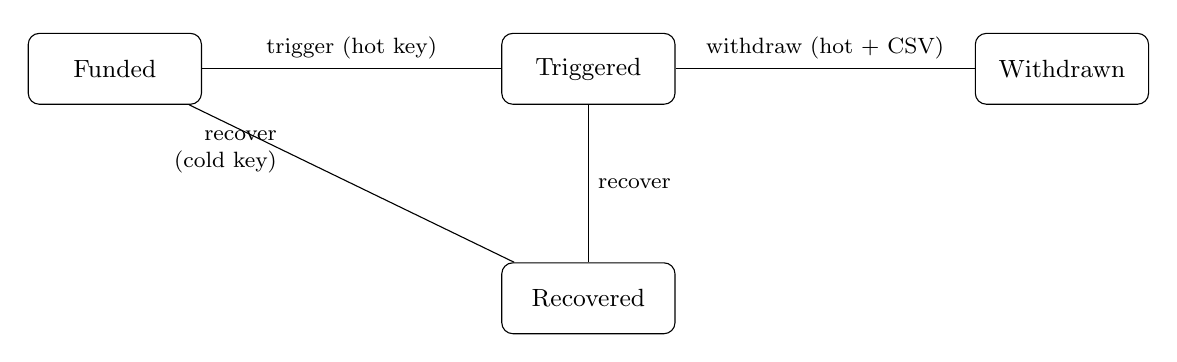
\begin{tikzpicture}[
  node distance=3.5cm and 3.8cm,
  state/.style={rectangle, draw, rounded corners, minimum width=2.2cm,
                minimum height=0.9cm, font=\small},
  every edge/.style={draw, ->, >=stealth, thick},
]
  \node[state] (funded) {Funded};
  \node[state, right=of funded] (triggered) {Triggered};
  \node[state, right=of triggered] (withdrawn) {Withdrawn};
  \node[state, below=2cm of triggered] (recovered) {Recovered};

  \draw (funded) -- node[above, font=\footnotesize] {trigger (hot key)} (triggered);
  \draw (triggered) -- node[above, font=\footnotesize] {withdraw (hot + CSV)} (withdrawn);
  \draw (funded) -- node[left, font=\footnotesize, align=right, pos=0.3] {recover\\(cold key)} (recovered);
  \draw (triggered) -- node[right, font=\footnotesize] {recover} (recovered);
\end{tikzpicture}
\caption{Vault lifecycle state machine. All covenant designs implement this four-state
model. The trigger-to-withdrawal transition enforces a relative timelock (CSV) that
creates the watchtower monitoring window. Recovery is available from both the Funded
and Triggered states.}
\label{fig:vault_lifecycle}
\end{figure}

The watchtower is an automated process that monitors the blockchain for unauthorized
trigger transactions. When the watchtower detects an unexpected unvault, it broadcasts
a recovery transaction during the CSV delay window. The security of the vault depends
on two assumptions: (1)~the watchtower is online and connected to the network during
the delay period, and (2)~the recovery transaction can confirm before the attacker's
withdrawal.

\subsection{Threat Model Assumptions (Kerckhoffs)}
\label{ss:kerckhoffs}

We adopt the standard cryptographic threat model. The adversary is
assumed to know the vault's design, the covenant type, the script
structure, and all public parameters --- including the recovery
address where applicable. Security rests on keys and on the script's
semantics, not on the secrecy of construction. Every attack-feasibility
claim in this thesis is evaluated under this assumption. Concretely,
we do not rely on taproot leaf hiding, address non-disclosure, or
closed-source construction as security mechanisms.

This threat model choice is load-bearing for every attack-class
derivation in Chapter~\ref{ch:security}. A reviewer may object to
individual class-susceptibility claims with ``but taproot hides that
leaf,'' or ``but the attacker would not know the cold address''; those
objections target the on-chain information-reveal layer, where the
thesis makes no cryptographic claim. The Kerckhoffs assumption moves
the debate from ``does taproot leak?'' (which it does not, in the
absence of legitimate recovery use) to ``should a vault's griefing or
theft immunity depend on the secrecy of its construction?'' (which,
by Kerckhoffs, it should not). A vault that is griefing-immune only
because the attacker does not know its cold address is not
cryptographically secure; it is obscured. The moment the recovery path
is ever legitimately used on-chain, the cold address is revealed
permanently. Security-by-obscurity is therefore not a principled
defence, and the thesis assumes an attacker who has passed the
obscurity threshold.

\subsection{Threat Taxonomy} \label{ss:threat_taxonomy}

We extend the threat model of Swambo et al.~\cite{SHMB20} with attack classes
specific to the four covenant designs. Table~\ref{tab:threat_summary} summarizes the
eleven threat models used throughout this thesis. Each threat model specifies the
adversary's capabilities (which keys are compromised), the attack mechanism, and the
worst-case outcome. The full threat model matrix with per-covenant severity ratings
appears in Chapter~\ref{ch:security}.

\begin{table}[t]
\centering
\caption{Threat taxonomy. Each row defines an adversary profile used in the security
analysis (Chapter~\ref{ch:security}).}
\label{tab:threat_summary}
\small
\begin{tabular}{@{}clll@{}}
\toprule
ID & Attack class & Adversary capability & Worst-case outcome \\
\midrule
TM1  & Fee pinning            & Hot key + network access    & Fund theft (CTV) \\
TM2  & Recovery griefing      & Varies by covenant          & Denial of service \\
TM3  & Trigger key theft      & Hot/trigger key             & Fund theft or DoS \\
TM4  & Watchtower exhaustion  & Hot key + capital           & Fund loss (dust) \\
TM5  & Trigger xpub theft     & OP\_VAULT trigger xpub      & Amplified TM3 \\
TM6  & Dual-key compromise    & Hot + cold/auth key         & Fund theft or DoS \\
TM7  & Address reuse          & None (user error)           & Stuck funds (CTV) \\
TM8  & CCV mode bypass        & Script knowledge            & Total fund loss \\
TM9  & Hot key redirection    & Hot key (CAT+CSFS)          & Griefing only \\
TM10 & Witness tampering      & Hot key (CAT+CSFS)          & Impossible \\
TM11 & Cold key theft         & Cold key (CAT+CSFS)         & Total fund theft \\
\bottomrule
\end{tabular}
\end{table}

% ======================================================================
\section{OP\_CHECKTEMPLATEVERIFY (CTV)} \label{se:ctv}

CTV~\cite{BIP119} constrains the spending transaction to match a committed template
hash. The hash covers: \texttt{nVersion}, \texttt{nLockTime}, \texttt{scriptSigs} hash,
input count, \texttt{nSequence} hash, output count, outputs hash, and the current
input's index. A script of the form \texttt{<hash> OP\_CHECKTEMPLATEVERIFY} succeeds
only if the spending transaction's template hash matches exactly.

CTV commits to the transaction's output structure but \emph{not} to which UTXOs are
consumed as inputs (input prevouts and amounts are excluded from the hash). This
design choice means the same CTV script can be satisfied by different input UTXOs,
enabling output-centric covenants. However, it also means a second deposit to the same
CTV address creates a UTXO that cannot satisfy the template---the committed output
amounts are derived from the original deposit, and a different deposit amount produces
a permanently unspendable UTXO.

The CTV vault uses a two-step transaction tree. The vault UTXO is encumbered by a bare
CTV script committing to the unvault transaction. The unvault transaction creates a
P2WSH output with two spending paths: a hot-key withdrawal after a CSV delay (the
normal path), and a CTV-committed cold sweep (the recovery path). Both paths include
an anchor output for CPFP fee bumping. The entire tree is deterministic---it can be
regenerated from key material and the original deposit amount without storing presigned
transactions.

\begin{figure}[t]
\centering
\resizebox{0.95\textwidth}{!}{%
\begin{tikzpicture}[
  utxo/.style={rectangle, draw, rounded corners=2pt, minimum width=2.8cm,
               minimum height=1.0cm, align=center, font=\footnotesize,
               fill=blue!5, draw=blue!60!black, thick},
  script/.style={rectangle, draw, rounded corners=1pt, minimum width=2.8cm,
                 minimum height=0.5cm, align=center, font=\scriptsize\ttfamily,
                 fill=yellow!20, draw=yellow!60!black},
  leaf/.style={rectangle, draw, rounded corners=2pt, minimum width=2.6cm,
               minimum height=0.9cm, align=center, font=\scriptsize, thick},
  anchorstyle/.style={rectangle, draw, rounded corners=2pt, minimum width=2.2cm,
                      minimum height=0.7cm, align=center, font=\scriptsize,
                      fill=orange!10, draw=orange!60!black, thick},
  note/.style={font=\scriptsize, align=center, text=gray!70!black},
  phase/.style={font=\scriptsize\bfseries, text=gray!60!black},
  edge/.style={draw, ->, >=stealth, thick},
  hashbox/.style={rectangle, draw, dashed, rounded corners=2pt,
                  align=left, font=\tiny\ttfamily,
                  fill=gray!3, inner sep=5pt},
]
  % Phase labels (top row)
  \node[phase] (pd) at (0, 2.2) {Deposit};
  \node[phase] (pt) at (4.2, 2.2) {Trigger};
  \node[phase] (pu) at (8.4, 2.2) {Unvault output};
  \node[phase] (ps) at (12.6, 2.2) {Spending paths};

  % Deposit: vault UTXO
  \node[utxo] (vault) at (0, 0.9) {Vault UTXO\\ \footnotesize 0.5 BTC};
  \node[script, below=0.05cm of vault] (vaultscript) {<H> OP\_CTV};

  % Trigger: unvault tx
  \node[utxo] (unvault) at (4.2, 0.9) {Unvault TX\\ \footnotesize template = H};

  % Unvault output: P2WSH with 2 leaves
  \node[utxo] (unvaultout) at (8.4, 0.9) {Unvault UTXO\\ \footnotesize 0.5 BTC − fees};
  \node[script, below=0.05cm of unvaultout] {P2WSH, 2 leaves};

  % Anchor output (separate row below the tx)
  \node[anchorstyle] (anchor) at (8.4, -1.6) {Anchor\\ \footnotesize 3{,}300 sats};

  % Spending paths (right column)
  \node[leaf, fill=green!10, draw=green!60!black] (withdraw) at (12.6, 1.5)
        {Withdraw\\ \scriptsize hot + CSV delay};
  \node[leaf, fill=red!10, draw=red!60!black] (cold) at (12.6, 0.1)
        {Cold Sweep\\ \scriptsize CTV-committed};

  % Arrows: vault -> unvault (trigger)
  \draw[edge] (vault.east) -- (unvault.west);
  \node[note, above=0.0cm of {(2.1,1.55)}] {spend = template $H$};

  % unvault -> unvaultout
  \draw[edge] (unvault.east) -- (unvaultout.west);

  % unvault -> anchor (dashed, fee-bump branch)
  \draw[edge, dashed, orange!70!black] (unvault.south) -- ++(0,-1.0) -| (anchor.north)
        node[pos=0.75, left, note, text=orange!70!black] {CPFP};

  % unvaultout -> two leaves
  \draw[edge, green!60!black] (unvaultout.east) -- ++(0.6,0) |- (withdraw.west);
  \draw[edge, red!60!black]   (unvaultout.east) -- ++(0.6,0) |- (cold.west);

  % Template hash note (placed low-left, out of other elements' way)
  \node[hashbox] (hashdef) at (0, -2.5)
        {\textbf{Template hash $H$ commits to:}\\
         nVersion, nLockTime,\\
         scriptSigs hash, input count,\\
         nSequence hash, output count,\\
         \textbf{outputs hash}, input index};
  \draw[->, dashed, gray!60] (vaultscript.south) -- (hashdef.north);

\end{tikzpicture}}
\caption{CTV vault mechanism. The vault UTXO is encumbered by a bare CTV hash $H$
that commits to the unvault transaction's entire output structure; any spend
whose template hash differs from $H$ fails. The unvault UTXO is a P2WSH script
with two Taproot leaves: a hot-key withdrawal gated by \texttt{OP\_CSV}, and a
CTV-committed cold sweep. A 3{,}300-sat anchor output enables CPFP fee bumping.}
\label{fig:ctv_mechanism}
\end{figure}

% ======================================================================
\section{OP\_CHECKCONTRACTVERIFY (CCV)} \label{se:ccv}

CCV~\cite{BIP443} verifies relationships between inputs, outputs, and
Taproot~\cite{BIP341, BIP342} contract structure. The opcode takes five arguments from the stack: optional state data, an
output or input index, an expected internal key, an expected taptree root, and a
\emph{mode} byte that controls which checks are performed. Mode~0 verifies the output's
scriptPubKey matches the expected Taproot structure. Mode~1 checks amounts. Mode~2
checks both. Mode~$-1$ verifies the current input rather than an output.

CCV operates at the per-output granularity: each invocation constrains a single output
(or input) by index. This is fundamentally different from CTV's all-outputs-at-once
commitment. The per-output model enables two capabilities absent in CTV: partial
withdrawal via \texttt{trigger\_and\_revault} (splitting a vault into a withdrawal
portion and a re-funded vault in one transaction) and batched triggers (combining
multiple vault UTXOs into a single trigger transaction).

The CCV vault combines CCV for state transitions with CTV for the final withdrawal
template. The trigger step stores a CTV hash into the contract state. The withdraw
path enforces a CSV timelock and executes \texttt{OP\_CHECKTEMPLATEVERIFY} against the
stored hash. Recovery is keyless---anyone can invoke the recover clause, which sends
funds to the pre-committed recovery address without requiring a signature.

An important design property: undefined CCV mode values (any value outside
$\{-1, 0, 1, 2\}$) trigger \texttt{OP\_SUCCESS}, making the entire script succeed
unconditionally. This is deliberate forward-compatibility behavior specified in
BIP-443 to enable future soft-fork extensions, but it creates a developer footgun:
a mode byte error silently disables all covenant enforcement.

\begin{figure}[t]
\centering
\resizebox{0.95\textwidth}{!}{%
\begin{tikzpicture}[
  utxo/.style={rectangle, draw, rounded corners=2pt, minimum width=2.7cm,
               minimum height=0.95cm, align=center, font=\footnotesize,
               fill=blue!5, draw=blue!60!black, thick},
  leaf/.style={rectangle, draw, rounded corners=1pt, minimum width=2.7cm,
               minimum height=0.5cm, align=center, font=\scriptsize\ttfamily,
               fill=yellow!20, draw=yellow!60!black},
  recleaf/.style={rectangle, draw, rounded corners=1pt, minimum width=2.7cm,
                  minimum height=0.5cm, align=center, font=\scriptsize\ttfamily,
                  fill=red!12, draw=red!60!black},
  opcode/.style={rectangle, draw, rounded corners=2pt, minimum width=3.1cm,
                 minimum height=1.4cm, align=center, font=\scriptsize,
                 fill=purple!8, draw=purple!60!black, thick},
  modebox/.style={rectangle, draw, rounded corners=2pt, dashed,
                  align=left, font=\tiny\ttfamily,
                  fill=gray!3, inner sep=5pt},
  phase/.style={font=\scriptsize\bfseries, text=gray!60!black, align=center},
  note/.style={font=\scriptsize, align=center, text=gray!70!black},
  edge/.style={draw, ->, >=stealth, thick},
]
  % Phase labels across top
  \node[phase] at (0, 3.5) {Deposit (2 leaves)};
  \node[phase] at (4.5, 3.5) {Per-output check};
  \node[phase] at (9.0, 3.5) {Trigger outputs};

  % Deposit: vault with TWO leaves (trigger + recover)
  \node[utxo] (vault) at (0, 2.3) {Vault UTXO\\ \footnotesize 0.5 BTC};
  \node[leaf, below=0.1cm of vault] (triggerleaf) {trigger leaf: OP\_CCV};
  \node[recleaf, below=0.1cm of triggerleaf] (recoverleaf) {recover leaf: keyless};

  % CCV opcode detail
  \node[opcode] (ccv) at (4.5, 2.0)
       {\textbf{OP\_CCV}\\
        \ttfamily mode $\in$ \{−1,0,1,2\}\\
        \ttfamily <idx, pk,\\ \ttfamily taptree, data>};

  % Split outputs (trigger path)
  \node[utxo] (revault) at (9.0, 2.8) {Revault UTXO\\ \footnotesize 0.3 BTC};
  \node[leaf, below=0.05cm of revault] {CCV (recursive)};

  \node[utxo, fill=green!10, draw=green!60!black] (wdraw) at (9.0, 1.1)
       {Withdraw UTXO\\ \footnotesize 0.2 BTC};
  \node[leaf, below=0.05cm of wdraw] {CTV + CSV};

  % Recovery output (separate lane, below)
  \node[utxo, fill=red!10, draw=red!60!black] (rec) at (9.0, -1.8)
       {Recovery UTXO\\ \footnotesize \textbf{keyless}};
  \node[leaf, below=0.05cm of rec] {fixed address};

  % ===== Trigger path: trigger leaf -> OP_CCV -> [revault, withdraw] =====
  \draw[edge] (triggerleaf.east) -- ++(0.3,0) |- (ccv.west)
        node[pos=0.6, above, note] {trigger};
  \draw[edge] (ccv.east) -- ++(0.5,0) |- (revault.west);
  \draw[edge] (ccv.east) -- ++(0.5,0) |- (wdraw.west);

  % ===== Recovery path: recover leaf -> Recovery UTXO (DIRECT, bypasses OP_CCV) =====
  \draw[edge, red!70!black, rounded corners=6pt]
       (recoverleaf.east) -- ++(0.3,0) -- ++(0,-1.3) -| (rec.south);
  \node[note, text=red!70!black] at (5.2, -1.6) {any party may invoke};

  % Mode legend — placed above-right of OP_CCV to avoid crossing the recovery path
  \node[modebox] (modes) at (5.2, 5.3)
       {\textbf{Mode semantics:}\\
        mode\,0: check spk of output[idx]\\
        mode\,1: check amount[idx]\\
        mode\,2: check both\\
        mode\,-1: check this input};
  \draw[->, dashed, purple!60!black] (modes.south) -- (ccv.north);

\end{tikzpicture}}
\caption{CCV vault mechanism. The vault UTXO is a Taproot with two leaves:
a \emph{trigger} leaf containing \texttt{OP\_CCV}, and a keyless \emph{recover}
leaf. Spending the trigger leaf invokes the per-output
\texttt{OP\_CHECKCONTRACTVERIFY} check, whose mode byte selects whether to
verify the scriptPubKey, the amount, both, or the current input. Taptree
preservation enables recursion, supporting partial withdrawal via
\texttt{trigger\_and\_revault}. Spending the recover leaf is permissionless
and sends funds to the pre-committed address without a signature.}
\label{fig:ccv_mechanism}
\end{figure}

% ======================================================================
\section{OP\_VAULT (BIP-345)} \label{se:opvault}

OP\_VAULT~\cite{BIP345} provides dedicated vault opcodes: \texttt{OP\_VAULT} controls
withdrawal initiation, and \texttt{OP\_VAULT\_RECOVER} enables authorized recovery.
Unlike CCV's generic contract verification, these opcodes encode vault-specific semantics
directly. Amount preservation (ensuring outputs account for all input value), automatic
revault (excess value beyond the withdrawal amount is re-locked), and recovery
authorization (requiring a \texttt{recoveryauth} key signature) are enforced at the
opcode level.

The OP\_VAULT design uses a three-key model: a \emph{trigger key} (derived from an xpub)
initiates withdrawals, a \emph{recoveryauth key} authorizes emergency recovery, and a
\emph{recovery address} (embedded in the vault's Taproot internal key tweak) is the
pre-committed destination for recovered funds. This three-key separation is unique among
the designs studied: CTV and CAT+CSFS use two keys (hot + cold), and CCV uses one
(trigger key; recovery is keyless).

A structural consequence of OP\_VAULT's design is the \emph{fee-input requirement}. The
opcode's value preservation rule requires that all input value be accounted for in
outputs. Since transaction fees are paid from input value, the vault UTXO alone cannot
cover fees without violating value preservation. The reference implementation solves this
by adding a separate fee-wallet UTXO as a second input to every trigger and recovery
transaction, adding 80--90\vB{} of overhead per transaction.

BIP-345 was withdrawn in early 2025 in favor of BIP-443~\cite{OB25}. We include it in
this comparison because (a)~it represents a distinct design philosophy (purpose-built
vs.\ generic covenants), (b)~the economic comparison with CCV quantifies the cost of
that design choice (36\% lifecycle overhead), and (c)~it serves as a historical reference
for the OP\_VAULT-to-CCV transition.

\begin{figure}[t]
\centering
\resizebox{0.95\textwidth}{!}{%
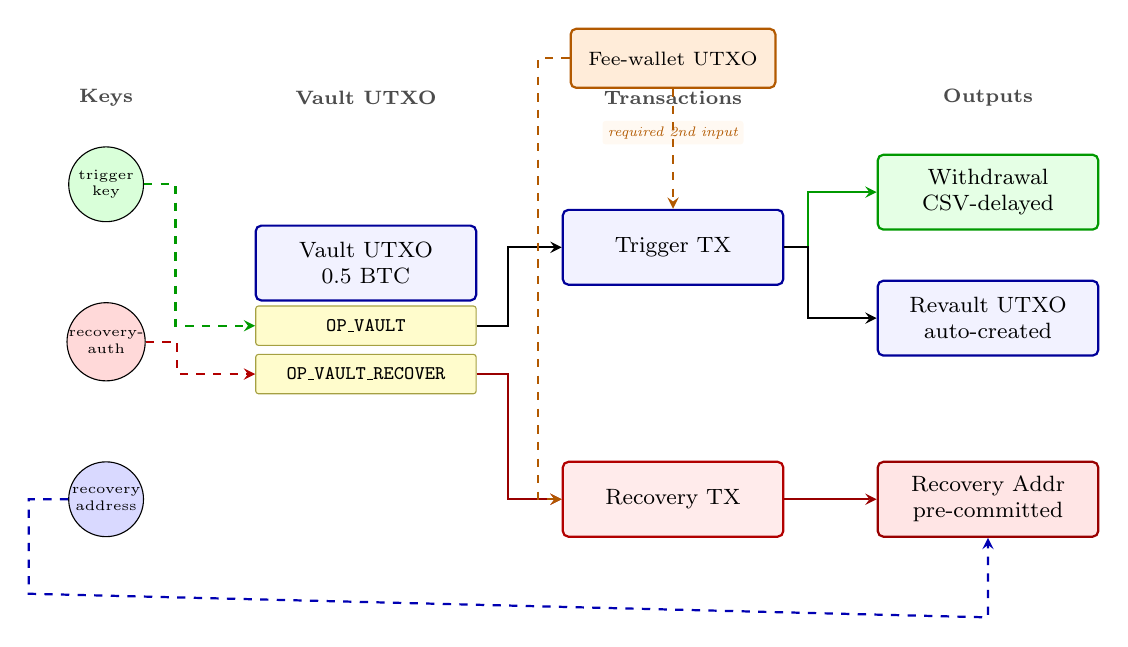
\begin{tikzpicture}[
  utxo/.style={rectangle, draw, rounded corners=2pt, minimum width=2.8cm,
               minimum height=0.95cm, align=center, font=\footnotesize,
               fill=blue!5, draw=blue!60!black, thick},
  fee/.style={rectangle, draw, rounded corners=2pt, minimum width=2.6cm,
              minimum height=0.75cm, align=center, font=\scriptsize,
              fill=orange!15, draw=orange!70!black, thick},
  leaf/.style={rectangle, draw, rounded corners=1pt, minimum width=2.8cm,
               minimum height=0.5cm, align=center, font=\scriptsize\ttfamily,
               fill=yellow!20, draw=yellow!60!black},
  keynode/.style={circle, draw, minimum size=0.95cm, font=\tiny, align=center,
              inner sep=0pt},
  phase/.style={font=\scriptsize\bfseries, text=gray!60!black, align=center},
  note/.style={font=\scriptsize, align=center, text=gray!70!black},
  edge/.style={draw, ->, >=stealth, thick},
]
  % Column x-coordinates
  \def\xkey{-0.2}
  \def\xvault{3.1}
  \def\xtx{7.0}
  \def\xout{11.0}

  % Phase labels
  \node[phase] at (\xkey, 3.4)   {Keys};
  \node[phase] at (\xvault, 3.4) {Vault UTXO};
  \node[phase] at (\xtx, 3.4)    {Transactions};
  \node[phase] at (\xout, 3.4)   {Outputs};

  % Three keys (left column)
  \node[keynode, fill=green!15] (tk) at (\xkey, 2.3) {trigger\\ key};
  \node[keynode, fill=red!15]   (ak) at (\xkey, 0.3) {recovery-\\ auth};
  \node[keynode, fill=blue!15]  (rk) at (\xkey, -1.7) {recovery\\ address};

  % Vault UTXO + two leaves
  \node[utxo] (vault) at (\xvault, 1.3) {Vault UTXO\\ \footnotesize 0.5 BTC};
  \node[leaf, below=0.05cm of vault] (tleaf) {OP\_VAULT};
  \node[leaf, below=0.1cm of tleaf] (rleaf) {OP\_VAULT\_RECOVER};

  % Fee wallet (above trigger)
  \node[fee] (feewallet) at (\xtx, 3.9) {Fee-wallet UTXO};
  \node[note, below=0.0cm of feewallet, yshift=-0.4cm, fill=orange!5,
        rounded corners=1pt, inner sep=2pt, font=\tiny\itshape, text=orange!70!black]
        {required 2nd input};

  % Trigger TX
  \node[utxo] (trigger) at (\xtx, 1.5) {Trigger TX};

  % Recovery TX (below)
  \node[utxo, fill=red!8, draw=red!70!black] (recovery) at (\xtx, -1.7) {Recovery TX};

  % Outputs
  \node[utxo, fill=green!10, draw=green!60!black] (wdraw) at (\xout, 2.2)
       {Withdrawal\\ \footnotesize CSV-delayed};
  \node[utxo] (revault2) at (\xout, 0.6) {Revault UTXO\\ \footnotesize auto-created};
  \node[utxo, fill=red!10, draw=red!60!black] (recdest) at (\xout, -1.7)
       {Recovery Addr\\ \footnotesize pre-committed};

  % Key authorization edges (dashed, short)
  \draw[edge, dashed, green!60!black] (tk.east) -- ++(0.4,0) |- (tleaf.west);
  \draw[edge, dashed, red!70!black]   (ak.east) -- ++(0.4,0) |- (rleaf.west);

  % Recovery-address key: routed below everything, up into recdest from below
  \draw[edge, dashed, blue!70!black]
       (rk.west) -- ++(-0.5,0) -- ++(0,-1.2)
       -- (\xout, -3.2) -- (recdest.south);

  % Vault -> Trigger
  \draw[edge] (tleaf.east) -- ++(0.4,0) |- (trigger.west);

  % Fee wallet -> Trigger (primary, dashed orange)
  \draw[edge, dashed, orange!70!black] (feewallet.south) -- (trigger.north);

  % Vault recover -> Recovery TX
  \draw[edge, red!60!black] (rleaf.east) -- ++(0.4,0) |- (recovery.west);

  % Fee wallet -> Recovery TX: route down the LEFT side so it doesn't cross Recovery Addr
  \draw[edge, dashed, orange!70!black]
       (feewallet.west) -- ++(-0.4,0) |- (recovery.west);

  % Trigger -> outputs
  \draw[edge, green!60!black] (trigger.east) -- ++(0.3,0) |- (wdraw.west);
  \draw[edge] (trigger.east) -- ++(0.3,0) |- (revault2.west);

  % Recovery -> dest
  \draw[edge, red!60!black] (recovery.east) -- (recdest.west);

\end{tikzpicture}}
\caption{OP\_VAULT mechanism. The opcode pair \texttt{OP\_VAULT} and
\texttt{OP\_VAULT\_RECOVER} encodes vault-specific semantics (amount preservation,
auto-revault, authorized recovery) directly. Three keys are separated: the
\emph{trigger key} initiates withdrawals, the \emph{recoveryauth key} authorizes
recovery, and the \emph{recovery address} (embedded in the Taproot internal-key
tweak) is the pre-committed destination. Value preservation requires a fee-wallet
input on every trigger and recovery transaction (${\sim}80$--$90\vB{}$ overhead).}
\label{fig:opvault_mechanism}
\end{figure}

% ======================================================================
\section{CAT+CSFS (BIP-347 + BIP-348)} \label{se:catcsfs_bg}

CAT+CSFS achieves transaction introspection by composing two general-purpose
opcodes~\cite{Poe21, BIP347, BIP348}. \texttt{OP\_CAT} (BIP-347) concatenates the top
two stack elements. \texttt{OP\_CHECKSIGFROMSTACK} (BIP-348) verifies a Schnorr
signature against an arbitrary stack-provided message rather than the transaction's
sighash. The introspection pattern works as follows:

\begin{enumerate}
\item The spender provides the sighash preimage fields (transaction version, hash
  prevouts, hash amounts, hash script pubkeys, hash sequences, hash outputs, spend
  type, and other BIP-342 fields) as individual witness elements.
\item The script uses \texttt{OP\_CAT} to assemble these fields into the complete
  sighash preimage on the stack.
\item \texttt{OP\_CHECKSIGFROMSTACK} verifies a Schnorr signature against this
  assembled preimage using the hot key.
\item \texttt{OP\_CHECKSIG} verifies the \emph{same signature} against the real
  transaction sighash computed by the Bitcoin consensus layer.
\end{enumerate}

If both checks pass with the same key and signature, the witness-provided preimage
must be the actual transaction's preimage (otherwise the signature could not satisfy
both). The script can embed constants (such as \texttt{sha\_single\_output}, the SHA-256
hash of the expected output) that the spender cannot alter, effectively constraining
the transaction's outputs through the signature binding.

The CAT+CSFS vault uses \texttt{SIGHASH\_SINGLE|ANYONECANPAY} (0x83), a sighash
mode defined in BIP-342~\cite{BIP342} that commits to one input and one output.
This allows external fee-paying inputs to be attached without breaking the
covenant---a more flexible fee model than CTV's anchor-based CPFP.

Two properties of this design have direct security implications. First, the withdrawal
destination is fixed at vault creation time (the \texttt{sha\_single\_output} constant
is embedded in the script), making it the most rigid destination constraint of any
design studied. Second, the recovery leaf uses bare \texttt{cold\_pk OP\_CHECKSIG}
with no introspection, meaning cold key compromise grants the attacker unrestricted
control over recovery---the weakest recovery path among the four Bitcoin designs.

\begin{figure}[t]
\centering
\resizebox{0.97\textwidth}{!}{%
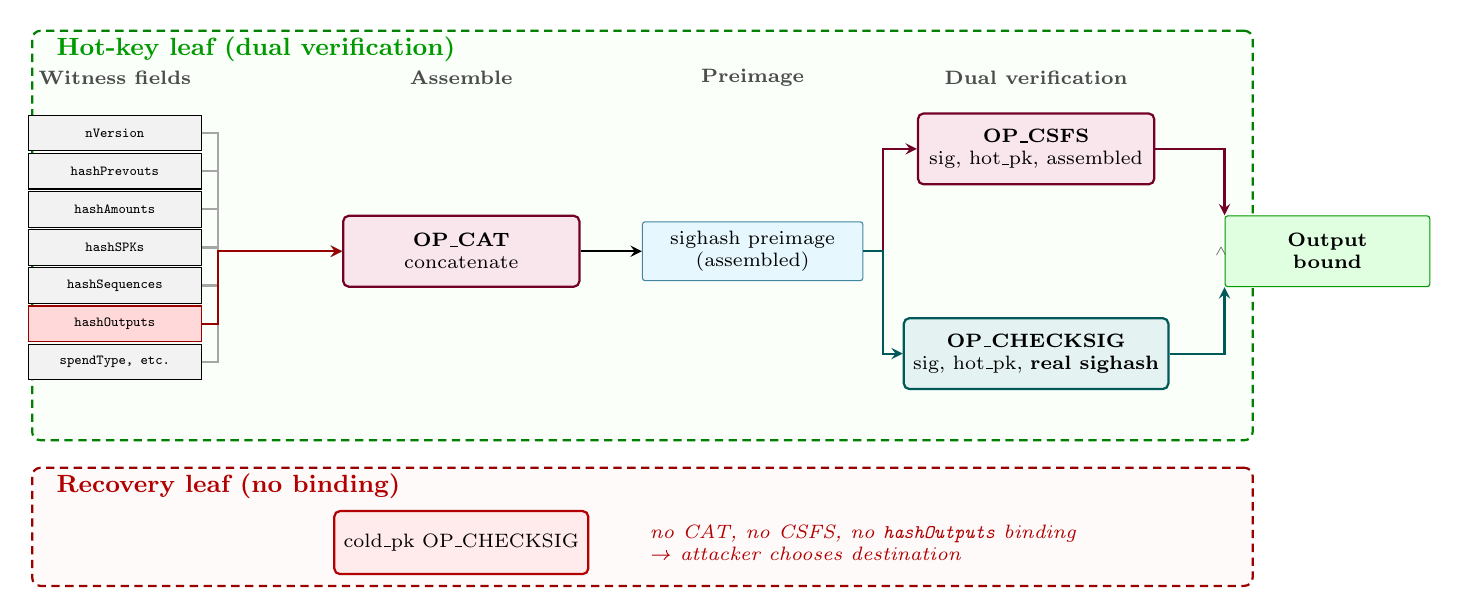
\begin{tikzpicture}[
  witness/.style={rectangle, draw, minimum width=2.2cm, minimum height=0.45cm,
                  font=\tiny\ttfamily, align=center, fill=gray!10},
  opbox/.style={rectangle, draw, rounded corners=2pt, minimum width=3.0cm,
                minimum height=0.9cm, align=center, font=\scriptsize,
                fill=purple!10, draw=purple!60!black, thick},
  sigbox/.style={rectangle, draw, rounded corners=1pt, minimum width=2.8cm,
                 minimum height=0.6cm, align=center, font=\scriptsize,
                 fill=cyan!10, draw=cyan!60!black},
  leafcontainer/.style={rectangle, draw, rounded corners=3pt, thick,
                        dash pattern=on 3pt off 2pt},
  bad/.style={rectangle, draw, rounded corners=2pt, minimum width=3.0cm,
              minimum height=0.8cm, align=center, font=\scriptsize,
              fill=red!8, draw=red!70!black, thick},
  note/.style={font=\scriptsize, align=center, text=gray!70!black},
  phase/.style={font=\scriptsize\bfseries, text=gray!60!black, align=center},
  edge/.style={draw, ->, >=stealth, thick},
]
  % ========= HOT LEAF (top container) =========
  \node[leafcontainer, fill=green!2, draw=green!50!black, minimum width=15.5cm,
        minimum height=5.2cm] (hotleaf) at (7.2, 0.7) {};
  \node[font=\small\bfseries, text=green!60!black, anchor=west]
       at ($(hotleaf.north west)+(0.2,-0.25)$) {Hot-key leaf (dual verification)};

  % Phase labels along hot leaf
  \node[phase] at (0.5, 2.7) {Witness fields};
  \node[phase] at (4.9, 2.7) {Assemble};
  \node[phase] at (8.6, 2.7) {Preimage};
  \node[phase] at (12.2, 2.7) {Dual verification};

  % Witness fields
  \node[witness] (w1) at (0.5, 2.0) {nVersion};
  \node[witness, below=0.02cm of w1] (w2) {hashPrevouts};
  \node[witness, below=0.02cm of w2] (w3) {hashAmounts};
  \node[witness, below=0.02cm of w3] (w4) {hashSPKs};
  \node[witness, below=0.02cm of w4] (w5) {hashSequences};
  \node[witness, below=0.02cm of w5, fill=red!15, draw=red!60!black]
       (w6) {\textbf{hashOutputs}};
  \node[witness, below=0.02cm of w6] (w7) {spendType, etc.};

  % OP_CAT
  \node[opbox] (cat) at (4.9, 0.5) {\textbf{OP\_CAT}\\ concatenate};

  % Preimage
  \node[sigbox] (preimage) at (8.6, 0.5) {sighash preimage\\ (assembled)};

  % OP_CSFS (upper)
  \node[opbox] (csfs) at (12.2, 1.8) {\textbf{OP\_CSFS}\\ \scriptsize sig, hot\_pk,
        assembled};
  % OP_CHECKSIG (lower)
  \node[opbox, fill=teal!10, draw=teal!70!black] (csig) at (12.2, -0.8)
       {\textbf{OP\_CHECKSIG}\\ \scriptsize sig, hot\_pk, \textbf{real sighash}};

  % Binding outcome (right of hot leaf, same level)
  \node[sigbox, fill=green!12, draw=green!60!black, minimum width=2.6cm,
        minimum height=0.9cm, font=\scriptsize\bfseries] (bind)
       at (15.9, 0.5) {Output\\ bound};

  % Edges inside hot leaf
  \foreach \i in {1,2,3,4,5,7} {
    \draw[edge, gray!70] (w\i.east) -- ++(0.2,0) |- (cat.west);
  }
  \draw[edge, red!60!black, thick] (w6.east) -- ++(0.2,0) |- (cat.west);

  \draw[edge] (cat) -- (preimage);
  \draw[edge, purple!60!black] (preimage.east) -- ++(0.25,0) |- (csfs.west);
  \draw[edge, teal!70!black] (preimage.east) -- ++(0.25,0) |- (csig.west);
  % Both verifications converge on Output bound's west face via L-shapes
  \draw[edge, purple!60!black] (csfs.east) -| (bind.north west);
  \draw[edge, teal!70!black]   (csig.east) -| (bind.south west);
  \node[font=\tiny\itshape, text=gray!70!black] at (14.55, 0.5) {$\wedge$};

  % ========= RECOVERY LEAF (bottom container, contrast) =========
  \node[leafcontainer, fill=red!2, draw=red!60!black, minimum width=15.5cm,
        minimum height=1.5cm] (coldleaf) at (7.2, -3.0) {};
  \node[font=\small\bfseries, text=red!70!black, anchor=west]
       at ($(coldleaf.north west)+(0.2,-0.25)$) {Recovery leaf (no binding)};

  \node[bad] (recoverbox) at (4.9, -3.2) {cold\_pk OP\_CHECKSIG};
  \node[note, text=red!70!black, align=left, font=\scriptsize\itshape]
       at (10.0, -3.2) {no CAT, no CSFS, no \texttt{hashOutputs} binding\\
                         → attacker chooses destination};

\end{tikzpicture}}
\caption{CAT+CSFS vault mechanism. The Taproot script has two leaves.
\textbf{Hot-key leaf (top):} the spender provides sighash preimage fields;
\texttt{OP\_CAT} concatenates them; \texttt{OP\_CSFS} verifies the Schnorr
signature against this stack-assembled preimage; \texttt{OP\_CHECKSIG} verifies
the \emph{same} signature against the real transaction sighash. Both succeed
only if the two preimages agree, binding outputs through \texttt{hashOutputs}.
\textbf{Recovery leaf (bottom):} bare \texttt{cold\_pk OP\_CHECKSIG}---no CAT,
no CSFS, no output binding.}
\label{fig:catcsfs_mechanism}
\end{figure}

% ======================================================================
\section{Simplicity on Elements: An Alternative Script Primitive} \label{se:simplicity_bg}

The four proposals above extend Bitcoin Script by introducing new
opcodes or composing existing ones under soft-fork consensus change.
Simplicity takes a different path: it is an \emph{alternative script
primitive}, a typed combinator calculus with denotational semantics
verified in the Coq proof assistant, designed by O'Connor~\cite{OC17}.
Programs are directed acyclic graphs (DAGs) of combinators. The
language runs on Elements/Liquid~\cite{DPNS16}, a federated Bitcoin
sidechain. Both Bitcoin Script and Simplicity are scripting languages;
they differ in paradigm (stack-based vs.\ typed functional), formal
foundation (informal specification vs.\ mechanised semantics), and
operating substrate (Bitcoin L1 proof-of-work vs.\ Elements federated
consensus).

Execution uses \emph{jets}: when the validator encounters a known combinator subtree
(identified by its canonical Merkle root), it executes a native C implementation instead
of interpreting the combinators. Jets for transaction introspection
(\texttt{jet::outputs\_hash()}, \texttt{jet::sig\_all\_hash()}), timelocks
(\texttt{jet::check\_lock\_distance()}), and cryptographic primitives
(\texttt{jet::bip\_0340\_verify()}~\cite{BIP340}) provide the building blocks for
covenant enforcement.

The Simplicity vault enforces covenants via \texttt{jet::outputs\_hash()}, which
computes a Merkle hash over all outputs of the spending transaction. The expected hash
is embedded as a compile-time parameter in the Simplicity program. At spend time, the
jet computes the hash from the actual transaction outputs; if the values differ, the
program fails at the consensus level. This is structurally analogous to CTV's template
hash but operates over Elements' richer output model (explicit asset IDs, confidential
values, range proofs).

The Simplicity vault runs on Elements, a federated sidechain where block production is
controlled by known functionaries rather than proof-of-work miners. This fundamentally
changes the trust model: functionaries could censor attacker transactions or collude
with an attacker, making the threat models (TM1--TM11) applicable only under the
assumption of honest federation behavior. Measurements from Elements are presented
separately from the four Bitcoin covenant measurements and are not directly comparable
due to differences in transaction serialization (explicit fee outputs, confidential
transaction fields add approximately 30--40 bytes per output).

\begin{figure}[t]
\centering
\resizebox{0.95\textwidth}{!}{%
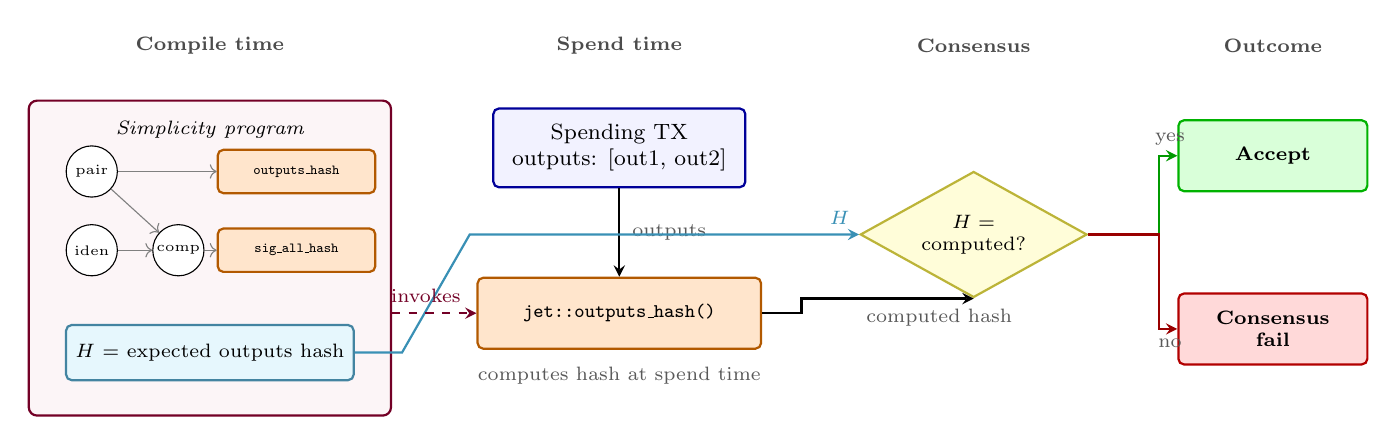
\begin{tikzpicture}[
  prog/.style={rectangle, draw, rounded corners=3pt, minimum width=4.6cm,
               minimum height=4.0cm, align=center, font=\scriptsize,
               fill=purple!4, draw=purple!60!black, thick},
  combinator/.style={circle, draw, minimum size=0.65cm, font=\tiny,
                     inner sep=0pt, fill=white},
  jetnode/.style={rectangle, draw, rounded corners=2pt, minimum width=2.0cm,
                  minimum height=0.55cm, font=\tiny, align=center,
                  fill=orange!20, draw=orange!70!black, thick},
  tx/.style={rectangle, draw, rounded corners=2pt, minimum width=3.2cm,
             minimum height=1.0cm, align=center, font=\footnotesize,
             fill=blue!5, draw=blue!60!black, thick},
  jetbig/.style={rectangle, draw, rounded corners=2pt, minimum width=3.6cm,
                 minimum height=0.9cm, font=\scriptsize, align=center,
                 fill=orange!20, draw=orange!70!black, thick},
  paramnodestyle/.style={rectangle, draw, rounded corners=2pt, minimum width=3.0cm,
                         minimum height=0.7cm, align=center, font=\scriptsize,
                         fill=cyan!10, draw=cyan!60!black, thick},
  checkbox/.style={diamond, draw, aspect=1.8, minimum width=2.4cm,
                   font=\scriptsize, align=center, thick,
                   fill=yellow!15, draw=yellow!70!black},
  outcome/.style={rectangle, draw, rounded corners=2pt, minimum width=2.4cm,
                  minimum height=0.9cm, align=center, font=\scriptsize\bfseries,
                  thick},
  phase/.style={font=\scriptsize\bfseries, text=gray!60!black, align=center},
  note/.style={font=\scriptsize, align=center, text=gray!70!black},
  edge/.style={draw, ->, >=stealth, thick},
]
  % ===== Phase headers (top, above all content) =====
  \node[phase] at (0, 3.9)    {Compile time};
  \node[phase] at (5.2, 3.9)  {Spend time};
  \node[phase] at (9.7, 3.9)  {Consensus};
  \node[phase] at (13.5, 3.9) {Outcome};

  % ===== Compile-time column: program with embedded H =====
  \node[prog] (program) at (0, 1.2) {};
  \node[font=\scriptsize\itshape, anchor=north]
       at ($(program.north)+(0,-0.15)$) {Simplicity program};

  % DAG mini-diagram (upper part of program)
  \node[combinator] (c1) at (-1.5, 2.3) {pair};
  \node[combinator] (c2) at (-1.5, 1.3) {iden};
  \node[combinator] (c3) at (-0.4, 1.3) {comp};
  \node[jetnode] (j1) at (1.1, 2.3) {\ttfamily outputs\_hash};
  \node[jetnode] (j2) at (1.1, 1.3) {\ttfamily sig\_all\_hash};
  \draw[->, thin, gray] (c1) -- (j1);
  \draw[->, thin, gray] (c3) -- (j2);
  \draw[->, thin, gray] (c2) -- (c3);
  \draw[->, thin, gray] (c1) -- (c3);

  % H parameter (lower part of program box)
  \node[paramnodestyle] (paramnode) at (0, 0.0) {$H$ = expected outputs hash};

  % ===== Spend-time column =====
  \node[tx] (spendtx) at (5.2, 2.6) {Spending TX\\ \footnotesize outputs: [out1, out2]};
  \node[jetbig] (jeteval) at (5.2, 0.5) {\ttfamily jet::outputs\_hash()};
  \node[note, below=0.1cm of jeteval, align=center, text width=4cm]
       {computes hash at spend time};

  % ===== Consensus column =====
  \node[checkbox] (check) at (9.7, 1.5) {$H =$\\ computed?};

  % ===== Outcome column =====
  \node[outcome, fill=green!15, draw=green!70!black] (ok) at (13.5, 2.5) {Accept};
  \node[outcome, fill=red!15, draw=red!70!black]   (fail) at (13.5, 0.3)
       {Consensus\\ fail};

  % ===== Edges =====
  % Spending TX -> jet (labeled "outputs")
  \draw[edge] (spendtx.south) -- (jeteval.north)
        node[midway, right=1pt, note] {outputs};

  % jet -> check (upper entry)
  \draw[edge] (jeteval.east) -- ++(0.5,0) |- (check.south)
        node[pos=0.9, below, note] {computed hash};

  % H -> check: route from paramnode top-right, rise to check level, into check.west
  \draw[edge, cyan!70!black]
       (paramnode.east) -- ++(0.6,0) -- (3.3, 1.5) -- (check.west)
       node[pos=0.95, above, note, text=cyan!70!black] {$H$};

  % Program "invokes" jet at spend time (dashed)
  \draw[edge, dashed, purple!60!black]
       (program.east |- jeteval.west) -- (jeteval.west)
       node[pos=0.4, above, note, text=purple!60!black] {invokes};

  % check -> outcomes
  \draw[edge, green!60!black] (check.east) -- ++(0.9,0) |- (ok.west)
        node[pos=0.8, above, note] {yes};
  \draw[edge, red!60!black]   (check.east) -- ++(0.9,0) |- (fail.west)
        node[pos=0.8, below, note] {no};

\end{tikzpicture}}
\caption{Simplicity vault mechanism on Elements. At compile time, the program
(a DAG of combinators) embeds an expected outputs-hash~$H$ as a parameter.
At spend time, \texttt{jet::outputs\_hash()} computes the Merkle hash of the
spending transaction's outputs. If the computed hash matches~$H$, the program
accepts; otherwise the program fails at the consensus level. Both trigger and
recovery leaves enforce this jet---unlike CAT+CSFS, where recovery is
unconstrained.}
\label{fig:simplicity_mechanism}
\end{figure}

\section{The Design-Space Axes}
\label{se:design_space_axes}

The four Bitcoin covenant proposals differ along seven axes.
Three carry over from the formal decomposition (\cite{SHMB20,Har24}
and this work) and appear with Greek-letter symbols $(f, a, g, b)$ in
proofs (Chapter~\ref{ch:security}); the remaining four are introduced
in this thesis and are used as descriptive labels. Every attack class
in Chapter~\ref{ch:security} derives from a specific axis-value;
every design's vulnerability profile is a lookup against
Table~\ref{tab:design_space_position}. We define the axes here, in
Background, so that Chapter~\ref{ch:security}'s analysis reads as
mechanical derivation rather than assertion.

\subsection{Axis Definitions}
\label{ss:axis_defs}

\begin{description}
\item[$\axauthf{}$ --- Recovery authorisation.] Who may initiate the
  recovery path? Values: \texttt{keyless}, \texttt{recoveryauth-key},
  \texttt{hot-key}, \texttt{cold-key}. Controls class \classgrief{}
  (permissionless griefing).

\item[$\axrevaultf{}$ --- Revault support.] Does the covenant allow
  partial withdrawal --- splitting one vault UTXO into a withdrawn
  output and a remaining vault UTXO in one transaction? Values:
  \texttt{yes}, \texttt{no}. Controls class \classscale{} (per-UTXO
  recovery-cost scaling).

\item[$\axfeef{}$ --- Fee-inclusion model.] Where does the spending
  transaction's fee come from? Values: \texttt{dynamic} (fee in the
  transaction), \texttt{static-precommit} (fee baked at creation),
  \texttt{out-of-band-anchor} (CPFP via a separate anchor key). Controls
  class \classfee{} (fee-channel pinning).

\item[\axwdbind{} --- Withdrawal-destination binding.] How is the
  withdrawal destination constrained? Values:
  \texttt{template-hash-digest}, \texttt{per-output-amount+script},
  \texttt{dedicated-opcode}, \texttt{signature-dual-bind}. Controls
  class \classhot{} (hot-key theft via destination substitution).

\item[\axrecbind{} --- Recovery-destination binding.] Same question
  for the recovery path. Values: same as \axwdbind{}, plus
  \texttt{plain-signature} (no script-level constraint). Controls
  class \classcold{} (cold-key theft via unconstrained recovery).
  Kept separate from \axwdbind{} because \catcsfs{} occupies different
  positions on the two sub-axes --- strongest on \axwdbind{}, weakest
  on \axrecbind{}. A collapsed binding axis $b$ is used in proofs that
  do not depend on this asymmetry.

\item[\axopsurf{} --- Opcode surface.] Is the covenant expressed by
  a single semantic opcode or a multi-mode polymorphic one with
  \texttt{OP\_SUCCESSx} fallthrough on undefined modes? Values:
  \texttt{single-mode}, \texttt{multi-mode-with-OP\_SUCCESS}. Controls
  class \classmode{} (mode/parameter bypass).

\item[\axintro{} --- Introspection primitive.] How does the script
  read transaction data? Values correspond to the four primitives
  enumerated in Section~\ref{se:introspection}:
  \texttt{digest-equality} (CTV),
  \texttt{merkle-membership-and-amount} (CCV),
  \texttt{dedicated-opcode} (OP\_VAULT), and
  \texttt{sighash-preimage-reconstruction} (CAT+CSFS). Descriptive;
  governs which of the other axes are simultaneously realisable.
\end{description}

For the formal decomposition in Chapter~\ref{ch:security} we retain
$(f, a, g, b)$ as the axes of the design-space lattice used in
Propositions~1 and~2: $f = \axfee$, $a = \axrevault$, $g = \axauth$,
and $b$ is the joint $(\axwdbind, \axrecbind)$ sublattice. Axes
\axopsurf{} and \axintro{} are additional dimensions orthogonal to
the proofs; they are where the developer-footgun (class \classmode{})
and design-implementability questions live.

\subsection{Four-Covenant Position Table}
\label{ss:position_table}

Table~\ref{tab:design_space_position} locates each of the four
Bitcoin proposals on every axis. Every attack-class
susceptibility claim in Chapter~\ref{ch:security} is a mechanical
lookup against this table; every immunity claim is a mechanical
reading of the opposite axis-value. Simplicity on Elements is
treated separately in Section~\ref{se:simplicity_bg} and (at greater
length) in Appendix~C; it occupies the strict-best position on
\axauth{}, \axrevault{}, \axwdbind{}, \axrecbind{}, and \axintro{}
simultaneously, and no Bitcoin proposal does.

\begin{table}[t]
\centering
\caption{The four Bitcoin covenant proposals, positioned on
the seven axes of Section~\ref{ss:axis_defs}. Every attack-class
susceptibility and immunity claim in Chapter~\ref{ch:security} is a
lookup against this table; numerical thresholds are measured in
Chapter~\ref{ch:results}.}
\label{tab:design_space_position}
\footnotesize
\setlength{\tabcolsep}{2.2pt}
\renewcommand{\arraystretch}{1.12}
\begin{tabular}{@{}lllll@{}}
\toprule
Axis                                    & \opctv{}               & \opccv{}                     & \opvault{}           & \catcsfs{}                      \\
\midrule
\axauth{} (recovery auth)               & hot-key                & keyless                      & recoveryauth-key     & cold-key                        \\
\axrevault{} (revault)                  & no                     & yes                          & yes                  & no                              \\
\axfee{} (fee model)                    & out-of-band-anchor     & dynamic                      & dynamic              & dynamic                         \\
\axwdbind{} (withdrawal binding)        & template-hash-digest   & per-output-amount+script     & dedicated-opcode     & signature-dual-bind             \\
\axrecbind{} (recovery binding)         & template-hash-digest   & per-output-amount+script     & dedicated-opcode     & plain-signature                 \\
\axopsurf{} (opcode surface)            & single-mode            & multi-mode-with-OP\_SUCCESS  & single-mode          & single-mode                     \\
\axintro{} (introspection primitive)    & digest-equality        & merkle-membership-and-amount & dedicated-opcode     & sighash-preimage-reconstruction \\
\bottomrule
\end{tabular}
\end{table}

\subsection{Structural Dependencies Between Axes}
\label{ss:axis_deps}

Two spec-level dependencies between axes constrain the realisable
combinations and are used throughout Chapter~\ref{ch:security}:

\begin{enumerate}
\item \axfee{} = \texttt{out-of-band-anchor} implies \axrevault{} =
  \texttt{no}. A CPFP-anchor fee model relies on a template hash
  that commits to the whole output set; splitting the vault into
  $[\text{withdrawn}] + [\text{remaining}]$ would require the
  template to anticipate the split amount, which the user cannot
  know at vault creation. CTV's position on these two axes is not
  coincidental; it is forced.

\item \axintro{} = \texttt{sighash-preimage-reconstruction} is the
  only known introspection primitive that admits \axwdbind{} =
  \texttt{signature-dual-bind}. The binding reduces to Schnorr
  message-equality under a single key, which requires reassembling
  the sighash preimage from stack contents and verifying two
  signatures under the same key --- a construction that the
  whole-template-digest, per-output, and dedicated-opcode primitives
  do not support.
\end{enumerate}

These dependencies reduce the effective design space from the naive
$4 \cdot 2 \cdot 3 \cdot 4 \cdot 5 \cdot 2 \cdot 4 = 1920$ cells to
a much smaller set of realisable positions. Every Bitcoin
proposal occupies a realisable position; the thesis contribution is
to characterise every realisable position's attack surface.

\chapter{Measurement Methodology} \label{ch:methodology}

This chapter describes how we measure and compare covenant vault designs.
Section~\ref{se:framework} presents the adapter-based framework architecture.
Section~\ref{se:metrics} defines the primary metric (virtual size) and the fee
projection model. Section~\ref{se:regtest_validity} analyzes what regtest measurements
do and do not tell us about mainnet behavior. Section~\ref{se:experiment_design}
catalogs the 15 experiments and their classification.
Section~\ref{se:node_infrastructure} documents the node variants required for each
covenant.

% ======================================================================
\section{Framework Architecture} \label{se:framework}

The comparison framework uses an \emph{adapter pattern} to decouple experiment logic
from covenant-specific implementations. Each vault design is wrapped in an adapter
class that implements a common interface (Figure~\ref{fig:architecture}). Experiments
invoke adapter methods---\texttt{create\_vault}, \texttt{trigger\_unvault},
\texttt{complete\_withdrawal}, \texttt{recover}---without knowledge of the underlying
covenant mechanism. This design serves two purposes: it ensures that measurements
across covenants use identical experiment logic, and it allows adding new covenant
designs without modifying existing experiments.

\begin{figure}[t]
\centering
\resizebox{0.9\textwidth}{!}{%
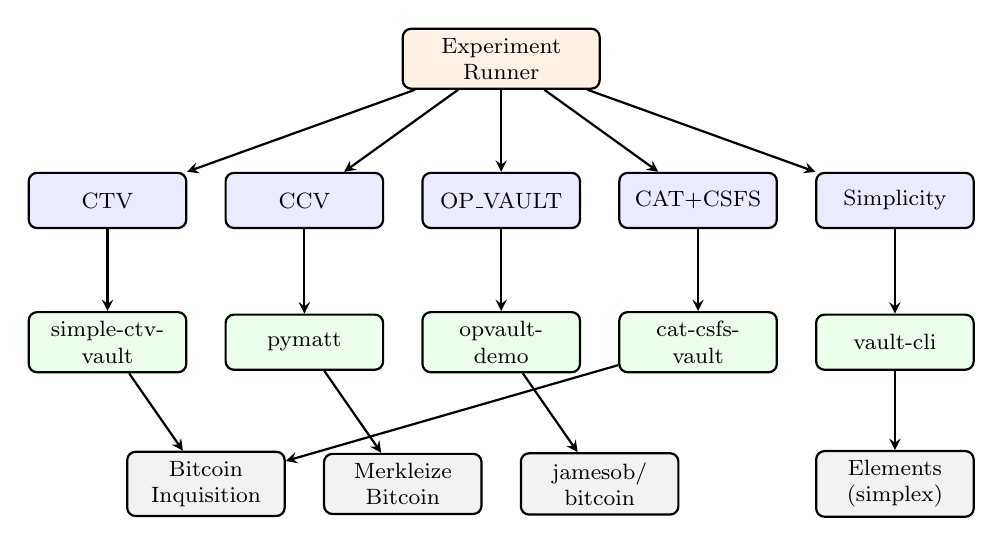
\begin{tikzpicture}[
  box/.style={rectangle, draw, rounded corners=3pt, minimum width=2cm,
              minimum height=0.7cm, font=\footnotesize, align=center},
  adapter/.style={box, fill=blue!8},
  node_box/.style={box, fill=gray!10},
  repo/.style={box, fill=green!8},
  >=stealth, thick,
]
  % Runner centered at top
  \node[box, minimum width=2.5cm, fill=orange!10] (runner) {Experiment\\Runner};

  % Adapters row — use explicit coordinates for even spacing
  \node[adapter] at (-5, -1.8) (ctv) {CTV};
  \node[adapter] at (-2.5, -1.8) (ccv) {CCV};
  \node[adapter] at (0, -1.8) (opv) {OP\_VAULT};
  \node[adapter] at (2.5, -1.8) (cat) {CAT+CSFS};
  \node[adapter] at (5, -1.8) (sim) {Simplicity};

  % Repos row
  \node[repo] at (-5, -3.6) (ctv_repo) {simple-ctv-\\vault};
  \node[repo] at (-2.5, -3.6) (ccv_repo) {pymatt};
  \node[repo] at (0, -3.6) (opv_repo) {opvault-\\demo};
  \node[repo] at (2.5, -3.6) (cat_repo) {cat-csfs-\\vault};
  \node[repo] at (5, -3.6) (sim_repo) {vault-cli};

  % Nodes row — 4 nodes, properly spaced
  % Inquisition centered between CTV and CAT positions
  \node[node_box] at (-3.75, -5.4) (inq) {Bitcoin\\Inquisition};
  \node[node_box] at (-1.25, -5.4) (merk) {Merkleize\\Bitcoin};
  \node[node_box] at (1.25, -5.4) (jamesob) {jamesob/\\bitcoin};
  \node[node_box] at (5, -5.4) (elements) {Elements\\(simplex)};

  % Arrows: runner to adapters
  \foreach \a in {ctv, ccv, opv, cat, sim}
    \draw[->] (runner) -- (\a);

  % Arrows: adapters to repos
  \foreach \a/\r in {ctv/ctv_repo, ccv/ccv_repo, opv/opv_repo, cat/cat_repo, sim/sim_repo}
    \draw[->] (\a) -- (\r);

  % Arrows: repos to nodes
  \draw[->] (ctv_repo) -- (inq);
  \draw[->] (cat_repo) -- (inq);
  \draw[->] (ccv_repo) -- (merk);
  \draw[->] (opv_repo) -- (jamesob);
  \draw[->] (sim_repo) -- (elements);
\end{tikzpicture}%
}
\caption{Framework architecture. The experiment runner invokes vault operations
through the \texttt{VaultAdapter} interface. Each adapter wraps a covenant-specific
implementation and communicates with its required Bitcoin or Elements node variant.
CTV and CAT+CSFS share the Bitcoin Inquisition node.}
\label{fig:architecture}
\end{figure}

\subsection{Adapter Interface} \label{ss:adapter_interface}

The abstract \texttt{VaultAdapter} class defines the contract that every adapter
must implement. The core lifecycle methods mirror the four-phase vault model from
Section~\ref{se:vault_lifecycle}:

\begin{itemize}
\item \texttt{create\_vault(amount\_sats)} $\rightarrow$ \texttt{VaultState}:
  Fund a new vault with the specified amount.
\item \texttt{trigger\_unvault(vault)} $\rightarrow$ \texttt{UnvaultState}:
  Initiate a withdrawal using the hot key.
\item \texttt{complete\_withdrawal(unvault)} $\rightarrow$ \texttt{TxRecord}:
  Finalize the withdrawal after the CSV delay.
\item \texttt{recover(state)} $\rightarrow$ \texttt{TxRecord}:
  Execute emergency recovery from either the Funded or Triggered state.
\end{itemize}

Optional methods expose capabilities that not all covenants support:
\texttt{trigger\_revault} for partial withdrawals (CCV, OP\_VAULT),
\texttt{trigger\_batched} for combining multiple vault UTXOs in one transaction
(CCV, OP\_VAULT), and \texttt{supports\_keyless\_recovery} for CCV's signature-free
recovery path.

\subsection{Capability-Based Dispatch} \label{ss:capability_dispatch}

Experiments query adapter capabilities at runtime rather than checking adapter names.
For example, the multi-input batching experiment calls
\texttt{adapter.supports\_batched\_trigger()} to determine whether to execute the
batched or linear code path. This design principle---dispatch on capabilities, not
identities---means a new adapter automatically participates in all experiments whose
required capabilities it declares. Table~\ref{tab:capabilities} shows the capability
matrix for the five adapters.

\begin{table}[t]
\centering
\caption{Adapter capability matrix. Experiments dispatch on these capabilities
rather than adapter names.}
\label{tab:capabilities}
\small
\begin{tabular}{@{}lccccc@{}}
\toprule
Capability & CTV & CCV & OPV & CAT & SIM \\
\midrule
\texttt{create\_vault}          & \checkmark & \checkmark & \checkmark & \checkmark & \checkmark \\
\texttt{trigger\_unvault}       & \checkmark & \checkmark & \checkmark & \checkmark & \checkmark \\
\texttt{complete\_withdrawal}   & \checkmark & \checkmark & \checkmark & \checkmark & \checkmark \\
\texttt{recover}                & \checkmark & \checkmark & \checkmark & \checkmark & \checkmark \\
\texttt{supports\_revault}      & ---        & \checkmark & \checkmark & ---        & ---        \\
\texttt{supports\_batched\_trigger} & ---    & \checkmark & \checkmark & ---        & ---        \\
\texttt{supports\_keyless\_recovery} & ---   & \checkmark & ---        & ---        & ---        \\
Address reuse safe              & No         & Yes        & Yes        & Yes        & Yes        \\
\bottomrule
\end{tabular}
\end{table}

\subsection{Implementation Provenance} \label{ss:provenance}

Three of the five vault implementations are third-party upstream repositories used
as-is: \texttt{simple-ctv-vault} (jamesob), \texttt{pymatt} (Merkleize/Ingala), and
\texttt{opvault-demo} (jamesob). The remaining two---\texttt{cat-csfs-vault} and
\texttt{simple-simplicity-vault}---are original implementations built for this research.
This distinction matters for interpreting results: implementation bugs in upstream
repositories are not attributable to the BIP design, while bugs in our own
implementations are indistinguishable from design choices unless explicitly documented.
Section~\ref{se:impl_choices} in Chapter~\ref{ch:discussion} lists the specific design
choices we made in the two original implementations.

% ======================================================================
\section{Primary Metric: Virtual Size} \label{se:metrics}

The primary metric throughout this work is \emph{virtual size} (vsize), measured in
virtual bytes (vB). Virtual size is the segwit-discounted transaction size used by
Bitcoin Core for relay policy, fee estimation, and block weight accounting:

\begin{equation} \label{eq:vsize}
\text{vsize} = \left\lceil \frac{\text{weight}}{4} \right\rceil
\quad \text{where} \quad
\text{weight} = 3 \times \text{base\_size} + \text{total\_size}
\end{equation}

\noindent
The base size excludes witness data; the total size includes it. The factor-of-4
discount on witness data reflects the segwit design decision to incentivize
witness-heavy transaction formats (Taproot, multisig) without increasing the block
size limit for non-witness data.

Virtual size is the correct metric for cross-covenant comparison because it is
\emph{structurally deterministic}: for a given script and witness structure, vsize
is identical regardless of chain state, balance, block height, or execution
environment. The per-UTXO recovery-cost scaling experiment (Chapter~\ref{ch:results})
confirmed this empirically: across 50 trigger-and-revault splits with vault
balances ranging from 50~million to fewer than 1{,}000 satoshis, the measured vsize
range was zero for both CCV and OP\_VAULT transactions.

This determinism has a methodological consequence: single-run measurements are
exact values, not estimates. There is no variance to analyze and no confidence
interval to compute. Repeated measurements would produce identical results because
the measurement is a function of the script structure, not a stochastic process.

\subsection{Fee Projection Model} \label{ss:fee_projection}

Since regtest has no fee market, we project transaction costs into real-world fee
environments using a linear model:

\begin{equation} \label{eq:fee_projection}
\text{fee}(r) = \text{vsize} \times r
\end{equation}

\noindent
where $r$ is the fee rate in sat/vB, treated as an exogenous parameter. We evaluate
all security experiments at six historically observed fee rates: 1~sat/vB (2021 low),
10~sat/vB (2022 average), 50~sat/vB (2023 moderate), 100~sat/vB (2024 inscriptions
era), 300~sat/vB (2023 BRC-20 spike), and 500~sat/vB (stress scenario). This
produces a cost sensitivity table for each attack, showing how the rationality
condition shifts across fee environments.

The rationality condition for an attack is:

\begin{equation} \label{eq:rationality}
\text{attack\_cost}(r) < \text{vault\_value}
\end{equation}

\noindent
An attack is economically rational when its on-chain cost (transaction fees plus
locked capital) is less than the value at risk in the vault. This condition is
necessary but not sufficient: the attacker must also expect the attack to succeed,
which depends on whether the defender's watchtower can respond within the CSV window.

% ======================================================================
\section{Rationality and Scope Conventions}
\label{se:rationality_conventions}

Every attack class derived in Chapter~\ref{ch:security} is accompanied
by a standardised \emph{Rationality and Scope} block with seven
fields. The fields are defined here, once, so that Chapter~\ref{ch:security}'s
derivations do not re-introduce the schema. Appendix~D carries the full
free-text form for every class; Chapter~\ref{ch:security} references
these blocks inline.

\begin{description}
\item[(1) Attacker capability.] Keys held, capital on hand, mempool
  access, compute. Cites the Kerckhoffs assumption of
  Section~\ref{ss:kerckhoffs} by reference; does not re-state it.
\item[(2) Defender model.] Watchtower authority and policy
  (proactive vs reactive, batched vs per-UTXO), user availability,
  detection-to-action latency. Where the attack depends on a specific
  defender choice, the block names it and explains why a rational
  defender might make that choice.
\item[(3) Economic preconditions.] Fee regime, vault-value range, and
  rationality threshold under which the attack yields positive
  adversary advantage.
\item[(4) Protocol / network assumptions.] Mempool policy parameters
  (descendant limits, dust thresholds, RBF rules), relay floor,
  TRUC/BIP-431 modifiers, cluster-mempool scope-limits.
\item[(5) Scope of validity.] Axis-values under which the class
  applies; equally important, the axis-values under which it does
  \emph{not} apply.
\item[(6) Rational-attacker check.] Is execution economically rational?
  Payoff vs cost vs residual (theft, liveness denial, both, or neither).
  If the attack is only rational under external incentive (extortion,
  competition, state actor), the block says so explicitly.
\item[(7) Counter-factual mitigations.] Which single falsified
  assumption kills the attack. This field doubles as a seed for
  deployment recommendations in Chapter~\ref{ch:discussion}.
\end{description}

The template applies to attack classes (Z1--Z6) in
Chapter~\ref{ch:security} and, with ``Attack'' replaced by
``Measurement'' in field (1), to empirical-cost measurements in
Chapter~\ref{ch:results}. Every field is populated, or explicitly
marked ``N/A --- [reason]''; partial blocks are treated as an audit
failure.

\section{Regtest Validity} \label{se:regtest_validity}

All experiments run on Bitcoin Core regtest (or Elements regtest for Simplicity). This
is a deliberate methodological choice: regtest provides deterministic, reproducible
execution without external dependencies. However, it limits external validity in
four specific ways.

\paragraph{No mempool competition.} Regtest mines transactions immediately on demand.
Attacks that depend on mempool dynamics---fee pinning races, front-running via mempool
observation, recovery races against timelocks---lose their temporal dimension. On
mainnet, a recovery transaction competes against the attacker's withdrawal for
confirmation within the CSV window.

\paragraph{No relay policy pressure.} Bitcoin Core's relay policy (descendant limits
at 25 transactions / 101~kvB, RBF rules, minimum relay fee) is enforced in regtest's
mempool but never stressed by competing traffic. The fee pinning experiment constructs
a 25-descendant chain that reaches the limit, but no concurrent transactions contest
for mempool space.

\paragraph{No fee market.} Fee amounts on regtest are artifacts of coin selection, not
rational economic behavior. This is why we treat vsize as the primary metric and
project fees via Equation~\ref{eq:fee_projection} rather than measuring them directly.

\paragraph{Mining is instant.} The CSV delay (e.g., 10 blocks $\approx$ 100 minutes on
mainnet) resolves in milliseconds on regtest. Time-critical races between the attacker's
withdrawal and the defender's recovery are instantaneous rather than uncertain.

Table~\ref{tab:regtest_validity} summarizes the validity status of each measurement
category on regtest.

\begin{table}[t]
\centering
\caption{Regtest validity. Structural properties transfer to mainnet; temporal and
economic dynamics do not.}
\label{tab:regtest_validity}
\small
\begin{tabular}{@{}lcc@{}}
\toprule
Property & Valid on regtest? & Primary limitation \\
\midrule
Transaction vsize and weight        & Yes (exact)     & --- \\
Script execution semantics          & Yes (identical) & --- \\
Descendant chain limits             & Yes (enforced)  & No competing traffic \\
Contract state transitions          & Yes (identical) & --- \\
Cost asymmetries (trigger vs.\ recovery) & Yes (structural) & --- \\
\midrule
Absolute fee amounts                & No (artifacts)  & No fee market \\
Recovery race timing                & No              & Instant mining \\
Mempool front-running               & No              & No competing traffic \\
Fee market confirmation pressure    & No              & No congestion \\
CSV manipulation via mining power   & No              & No adversarial miners \\
\bottomrule
\end{tabular}
\end{table}

% ======================================================================
\section{Experiment Catalog} \label{se:experiment_design}

The framework includes 15 experiments organized by scope and concern.
Table~\ref{tab:experiment_catalog} lists all experiments with their scope category,
the covenants they test, and the threat model they address.

Experiments fall into five scope categories:

\begin{itemize}
\item \textbf{Comparative.} The same test runs on all covenants; findings emerge from
  the differences in outcomes (A, B, C, F, H).
\item \textbf{Capability gap.} Tests a feature that some covenants support and others
  cannot (D, E).
\item \textbf{Covenant-specific.} Measures economic costs of design tradeoffs unique
  to one covenant (K, L, O, P).
\item \textbf{Verification.} Empirically confirms that specified opcode or
  cryptographic behavior holds in the implementation (I, M, N). These are
  implementation correctness checks, not security findings.
\item \textbf{Analytical.} Fee projections and sensitivity analysis using structural
  vsize as input; no on-chain transactions produced (J).
\end{itemize}

\begin{table}[t]
\centering
\caption{Experiment catalog. Each experiment is identified by a letter (A--P, no G)
and classified by scope and concern.}
\label{tab:experiment_catalog}
\small
\begin{tabular}{@{}cllll@{}}
\toprule
ID & Name & Category & Covenants & TM \\
\midrule
A & \texttt{lifecycle\_costs}     & Comparative   & All 5  & --- \\
B & \texttt{address\_reuse}       & Comparative   & All 5  & TM7 \\
C & \texttt{fee\_pinning}         & Comparative   & All 5  & TM1 \\
D & \texttt{revault\_amplification} & Capability gap & CCV, OPV & --- \\
E & \texttt{multi\_input}         & Capability gap & All 5  & --- \\
F & \texttt{recovery\_griefing}   & Comparative   & All 5  & TM2 \\
H & \texttt{watchtower\_exhaustion} & Comparative & CCV, OPV & TM4 \\
I & \texttt{ccv\_mode\_bypass}    & Verification  & CCV    & TM8 \\
J & \texttt{fee\_sensitivity}     & Analytical    & All    & All \\
K & \texttt{opvault\_recovery\_auth} & Covenant-specific & OPV & TM2 \\
L & \texttt{opvault\_trigger\_key\_theft} & Covenant-specific & OPV & TM3,5 \\
M & \texttt{cat\_csfs\_hot\_key\_theft} & Verification & CAT & TM9 \\
N & \texttt{cat\_csfs\_witness\_manip.} & Verification & CAT & TM10 \\
O & \texttt{cat\_csfs\_dest\_lock} & Covenant-specific & CAT & --- \\
P & \texttt{cat\_csfs\_cold\_key\_recovery} & Covenant-specific & CAT & TM11 \\
\bottomrule
\end{tabular}
\end{table}

% ======================================================================
\section{Node Infrastructure} \label{se:node_infrastructure}

Each covenant requires a specific Bitcoin (or Elements) node variant, because the
opcodes are not yet activated on Bitcoin mainnet. CTV and CAT+CSFS share Bitcoin
Inquisition, a soft-fork testing fork maintained by the Bitcoin Inquisition project.
CCV requires a separate fork maintained by Merkleize (Ingala). OP\_VAULT requires
jamesob's fork with the \texttt{2023-02-opvault-inq} branch, which uses the older
autotools build system. Simplicity runs on Elements via the Simplex toolchain, which
bundles \texttt{elementsd} and an Esplora block indexer.

\begin{table}[t]
\centering
\caption{Node variants required for each covenant. Switching nodes wipes regtest
state; experiments are isolated per-covenant.}
\label{tab:nodes}
\small
\begin{tabular}{@{}llll@{}}
\toprule
Covenant & Node variant & Branch & Build \\
\midrule
CTV       & Bitcoin Inquisition       & \texttt{v29.2-inq} release    & Pre-built \\
CCV       & Merkleize Bitcoin         & \texttt{inq-ccv}              & CMake \\
OP\_VAULT & jamesob/bitcoin           & \texttt{2023-02-opvault-inq}  & Autotools \\
CAT+CSFS  & Bitcoin Inquisition       & \texttt{v29.2-inq} release    & Pre-built \\
Simplicity & Elements (Simplex SDK)   & \texttt{v0.0.2}               & Pre-built \\
\bottomrule
\end{tabular}
\end{table}

The framework's \texttt{switch-node.sh} script manages node lifecycle: starting the
correct node variant, wiping regtest state between runs, and discovering ports for
Elements (which assigns random RPC and Esplora ports at startup). A Docker image
packages all five node variants with pre-built binaries for reproducible execution
without local compilation.

\chapter{Empirical Results} \label{ch:results}

This chapter presents the measured transaction sizes and cost data that form the
empirical basis for the security analysis in Chapter~\ref{ch:security}.
Section~\ref{se:lifecycle_measurements} reports the core lifecycle vsize measurements.
Section~\ref{se:opvault_correction} documents the correction of prior OP\_VAULT
estimates. Section~\ref{se:batching_results} presents batching efficiency data.
Section~\ref{se:revault_results} measures revault amplification costs.
Section~\ref{se:address_reuse_results} reports address reuse behavior.
Section~\ref{se:simplicity_measurements} presents the Simplicity vault measurements
separately.

% ======================================================================
\section{Lifecycle Cost Measurements} \label{se:lifecycle_measurements}

Table~\ref{tab:lifecycle} shows the measured vsize for each transaction in the
deposit--trigger--withdraw lifecycle across all five covenant designs. These
measurements are the foundation for all subsequent cost analysis: every attack cost
function, fee sensitivity projection, and cross-covenant comparison in this thesis
derives from these structural vsize values.

\begin{table}[t]
\centering
\caption{Lifecycle vsize measurements for the four Bitcoin
covenant designs. Each value is regtest-measured and structurally
deterministic (range = 0 across repeated measurements). Lifecycle
total = tovault + trigger + withdraw (the happy-path cost). Simplicity
(Elements) measurements appear in Appendix~C. The \emph{axis measured}
column identifies the primary axis
(Table~\ref{tab:design_space_position}) whose position determines the
row's cost structure.}
\label{tab:lifecycle}
\begin{tabular}{@{}lrrrrcl@{}}
\toprule
Covenant & tovault & trigger & withdraw & recover & \textbf{total}  & axis measured                                                 \\
         & (vB)    & (vB)    & (vB)     & (vB)    & \textbf{(vB)}   &                                                               \\
\midrule
CTV        & 122 &  94 & 152 & 133 & \textbf{368} & \axfee{}=anchor, \axwdbind{}=digest          \\
CCV        & 300 & 154 & 111 & 122 & \textbf{565} & \axrevault{}=yes, \axfee{}=dynamic           \\
OP\_VAULT  & 154 & 292 & 121 & 246 & \textbf{567} & \axrevault{}=yes, \axfee{}=dynamic (wallet)  \\
CAT+CSFS   & 122 & 221 & 210 & 125 & \textbf{553} & \axwdbind{}=dual-bind, \axfee{}=ACP          \\
\bottomrule
\end{tabular}
\end{table}

CTV has the cheapest lifecycle at 368\vB{}, owing to its minimal script structure: the
trigger (unvault) transaction is a bare CTV hash check with no signature, producing
the smallest trigger of any design at 94\vB{}. CCV and OP\_VAULT have nearly identical
lifecycle totals (565 and 567\vB{}), but with opposite cost distributions: CCV's
trigger is cheap (154\vB{}) and its deposit is expensive (300\vB{} due to the
two-output contract instance structure), while OP\_VAULT's trigger is expensive
(292\vB{} due to the fee-wallet input) and its deposit is moderate (154\vB{}).
CAT+CSFS falls between CTV and CCV/OP\_VAULT at 553\vB{}, with the dual CSFS+CHECKSIG
introspection pattern adding witness overhead to both trigger (221\vB{}) and withdrawal
(210\vB{}).

The lifecycle cost at a given fee rate~$r$ (in sat/vB) is:

\begin{equation} \label{eq:lifecycle_cost}
C_{\text{lifecycle}}(r) = (\text{vsize}_{\text{tovault}} + \text{vsize}_{\text{trigger}}
  + \text{vsize}_{\text{withdraw}}) \times r
\end{equation}

\noindent
At the median 2024 fee rate of 50\satvB{}, a single vault lifecycle costs 18{,}400~sats
(CTV), 28{,}250~sats (CCV), 28{,}350~sats (OP\_VAULT), or 27{,}650~sats (CAT+CSFS).

% ======================================================================
\section{OP\_VAULT Vsize Correction} \label{se:opvault_correction}

Prior to this work, the only published transaction size estimates for OP\_VAULT were
informal hand-calculations. Table~\ref{tab:opvault_correction} compares these estimates
against our regtest measurements.

\begin{table}[t]
\centering
\caption{OP\_VAULT vsize corrections. Prior estimates are from informal community
discussion; measured values are from regtest lifecycle runs on the
\texttt{opvault-demo} reference implementation.}
\label{tab:opvault_correction}
\begin{tabular}{@{}lrrr@{}}
\toprule
Transaction & Prior estimate & Measured & Delta \\
\midrule
trigger (\texttt{start\_withdrawal})  & ${\sim}200$\vB{} & 292\vB{} & $+46\%$ \\
recovery (\texttt{OP\_VAULT\_RECOVER}) & ${\sim}170$\vB{} & 246\vB{} & $+45\%$ \\
\bottomrule
\end{tabular}
\end{table}

The discrepancy originates from the fee-input requirement described in
Section~\ref{se:opvault}. OP\_VAULT's value preservation rule prohibits spending the
vault UTXO alone (the fee would violate input--output balance), so every trigger and
recovery transaction includes a second input from a fee wallet. This adds a P2TR
input witness (approximately 80--90\vB{}) that prior estimates omitted. The
consequence is a 36\% lifecycle cost premium over CCV: OP\_VAULT's lifecycle
(567\vB{}) versus CCV's (565\vB{}) appears similar in total, but OP\_VAULT pays
80--90\vB{} more for every non-deposit transaction. Over time, the accumulated
overhead is significant for vault operators who trigger frequently.

This measurement contributed to the economic case for withdrawing BIP-345 in favor
of BIP-443~\cite{OB25}: the purpose-built opcodes' fee-input overhead costs more
than the generic CCV approach achieves with the same vault semantics.

% ======================================================================
\section{Batching Efficiency} \label{se:batching_results}

CCV and OP\_VAULT can combine multiple vault UTXOs into a single trigger transaction.
CTV and CAT+CSFS cannot batch because each vault's template hash (CTV) or embedded
\texttt{sha\_single\_output} (CAT+CSFS) commits to a specific output structure that
changes with each additional input.

Table~\ref{tab:batching} shows the measured trigger vsize at increasing batch sizes.
Both CCV and OP\_VAULT exhibit linear scaling with a fixed base cost and a constant
marginal cost per additional vault.

\begin{table}[t]
\centering
\caption{Batched trigger vsize measurements. CCV and OP\_VAULT are measured from
actual multi-input transactions on regtest. CTV and CAT+CSFS cannot batch.}
\label{tab:batching}
\begin{tabular}{@{}lrrrrrr@{}}
\toprule
& \multicolumn{6}{c}{Batch size ($N$ vaults)} \\
\cmidrule(l){2-7}
Covenant & $N{=}1$ & $N{=}2$ & $N{=}3$ & $N{=}5$ & $N{=}10$ & $N{=}20$ \\
\midrule
CCV       & 154 & 254  & 355   & 555   & 1{,}056  & 2{,}059 \\
OP\_VAULT & 292 & 385  & 479   & 667   & 1{,}135  & 2{,}073 \\
\midrule
\multicolumn{7}{@{}l}{\footnotesize CTV, CAT+CSFS: $N \times$ single trigger
(154\vB{}, 221\vB{} respectively)} \\
\bottomrule
\end{tabular}
\end{table}

The batching efficiency follows a linear model:

\begin{equation} \label{eq:batching}
\text{vsize}_{\text{batch}}(N) = \text{base} + \text{marginal} \times N
\end{equation}

\noindent
For CCV, the marginal cost is ${\sim}100$\vB{} per additional vault (base
${\sim}54$\vB{}). For OP\_VAULT, the marginal cost is ${\sim}94$\vB{} per vault
(base ${\sim}198$\vB{}). The marginal cost per vault in a batch is substantially
lower than the cost of individual triggers (154\vB{} for CCV, 292\vB{} for
OP\_VAULT), demonstrating the efficiency gain from amortizing the transaction
overhead across multiple inputs.

The standardness ceiling---the maximum batch size that fits within Bitcoin Core's
400{,}000~WU transaction weight limit---can be projected from these measurements:

\begin{equation} \label{eq:ceiling}
N_{\max} = \left\lfloor \frac{400{,}000 - \text{base\_weight}}
  {\text{marginal\_weight}} \right\rfloor
\end{equation}

\noindent
For CCV, $N_{\max} \approx 1{,}000$ vaults per transaction. For OP\_VAULT,
$N_{\max} \approx 1{,}064$ vaults. In practice, batch sizes above 50--100 are rare
in custodial operations, so the standardness limit does not constrain realistic
deployments.

% ======================================================================
\section{Revault Amplification} \label{se:revault_results}

CCV and OP\_VAULT support partial withdrawals: the vault owner withdraws a portion
of the vault balance and re-locks the remainder in a new vault UTXO. This process
can be repeated, creating a chain of partial withdrawals from a single initial
deposit.

The cost of each withdrawal step is the sum of the trigger (or trigger-and-revault)
and the withdrawal completion. Table~\ref{tab:revault} shows the per-step and
cumulative costs measured across 9~successive partial withdrawals of 5{,}000{,}000~sats
each from an initial 49{,}999{,}900-sat vault.

\begin{table}[t]
\centering
\caption{Revault amplification. Per-step withdrawal vsize is constant across steps
because the script structure does not change with balance. CTV and CAT+CSFS cannot
revault natively; their cost is the full unvault--withdraw cycle per withdrawal.}
\label{tab:revault}
\begin{tabular}{@{}lrrr@{}}
\toprule
Covenant & Per-step vsize & Cumulative (5 steps) & Cumulative (9 steps) \\
\midrule
CCV       & 111\vB{} & 555\vB{} & 999\vB{} \\
OP\_VAULT & 121\vB{} & 605\vB{} & 1{,}089\vB{} \\
\midrule
CTV (extrapolated)      & 246\vB{} & 1{,}230\vB{} & 2{,}214\vB{} \\
CAT+CSFS (extrapolated) & 431\vB{} & 2{,}155\vB{} & 3{,}879\vB{} \\
\bottomrule
\end{tabular}
\end{table}

The per-step vsize is constant across all 9~steps for both CCV and OP\_VAULT, confirming
the structural determinism of the measurement. CCV's smaller per-step cost (111\vB{}
vs.\ 121\vB{}) reflects its lighter withdrawal transaction (no fee-input overhead).

For CTV and CAT+CSFS, which lack native revault, each partial withdrawal requires a
full cycle: unvault the entire balance, withdraw the desired portion, and re-deposit
the remainder in a new vault. The extrapolated per-step cost is the sum of the trigger
and withdrawal vsizes for a single cycle. This is 2.2$\times$ (CTV) to 3.9$\times$
(CAT+CSFS) more expensive than CCV's native revault per step.

The cumulative cost has implications for the per-UTXO recovery-cost scaling attack analyzed in
Chapter~\ref{ch:security}: an attacker chaining many small partial withdrawals forces
the watchtower to pay recovery fees proportional to the number of splits.

% ======================================================================
\section{Address Reuse} \label{se:address_reuse_results}

CTV is the only design where address reuse causes permanent fund loss. A second deposit
to the same CTV address creates a UTXO whose amount does not match the committed
template hash. The template commits to output amounts derived from the \emph{original}
deposit, so the second UTXO is either permanently unspendable (if the deposit is
smaller) or overpays miners by the difference (if larger).

CCV, OP\_VAULT, CAT+CSFS, and Simplicity all handle multiple deposits to the same
address safely. CCV and OP\_VAULT use per-instance contract checking---each UTXO is
independently validated against the covenant rules regardless of how many UTXOs share
the same address. CAT+CSFS generates a unique vault plan per source coin, producing
distinct P2TR addresses. Simplicity creates fresh plans with new addresses for each
vault instance.

This is a design-level property, not an implementation artifact: CTV's template hash
commits to input count and output amounts, making it structurally incompatible with
variable deposit amounts. The other designs either validate per-input (CCV, OP\_VAULT)
or per-instance (CAT+CSFS, Simplicity).

% ======================================================================
\section{Fee Sensitivity Projections} \label{se:fee_sensitivity_results}

Experiment~J projects the measured vsize data from the preceding sections into
real-world fee environments using the linear fee model
(Equation~\ref{eq:fee_projection}). Table~\ref{tab:fee_sensitivity} shows the
lifecycle cost and key attack costs across six historically observed fee rates.

\begin{table}[t]
\centering
\caption{Fee sensitivity projections. Lifecycle cost =
$\text{vsize}_{\text{total}} \times r$. Fee pinning cost is fee-invariant.
Recovery griefing cost is the defender's per-round cost. Watchtower exhaustion
shows the number of splits needed to exhaust a 0.5~BTC vault to dust.}
\label{tab:fee_sensitivity}
\footnotesize
\begin{tabular}{@{}rrrrrrrr@{}}
\toprule
& \multicolumn{4}{c}{Lifecycle cost (sats)} & Fee pin & Grief & WT exhaust \\
\cmidrule(lr){2-5}
$r$ (sat/vB) & CTV & CCV & OPV & CAT & (CTV) & (CCV) & splits \\
\midrule
1   &     368 &     565 &     567 &     553 & 14{,}300 &    454 & 409{,}836 \\
10  &   3{,}680 &   5{,}650 &   5{,}670 &   5{,}530 & 14{,}300 &  4{,}540 &  40{,}984 \\
50  &  18{,}400 &  28{,}250 &  28{,}350 &  27{,}650 & 14{,}300 & 22{,}700 &   8{,}197 \\
100 &  36{,}800 &  56{,}500 &  56{,}700 &  55{,}300 & 14{,}300 & 45{,}400 &   4{,}098 \\
300 & 110{,}400 & 169{,}500 & 170{,}100 & 165{,}900 & 14{,}300 & 136{,}200 &  1{,}366 \\
500 & 184{,}000 & 282{,}500 & 283{,}500 & 276{,}500 & 14{,}300 & 227{,}000 &    820 \\
\bottomrule
\end{tabular}
\end{table}

Three observations emerge from the projections:

\begin{itemize}
\item \textbf{Fee pinning is fee-invariant.} The 14{,}300-sat pinning cost
  (Section~\ref{se:fee_pinning}) is constant across all fee environments because
  the attacker pays dust-rate fees regardless of prevailing rates. At a 0.5~BTC
  vault value, pinning costs 0.03\% of the vault---well below any rationality
  threshold at any historical fee rate.

\item \textbf{Lifecycle cost rankings are stable.} CTV is the cheapest at every fee
  rate. CCV and OP\_VAULT are nearly identical (within 0.4\%). CAT+CSFS falls between
  CTV and CCV/OP\_VAULT. The ranking does not change with fees because the vsize
  ratios are constant.

\item \textbf{Watchtower exhaustion feasibility is fee-dependent.} At 1\satvB{},
  exhausting a 0.5~BTC vault requires ${\sim}410{,}000$ splits (infeasible---66 blocks
  of maximum-rate splitting). At 300\satvB{}, it requires only 1{,}366 splits
  (feasible in a single block). This fee-dependent transition is the empirical basis
  for Proposition~\ref{thm:fee_inversion} in Chapter~\ref{ch:security}.
\end{itemize}

% ======================================================================
\section{Synthesis: What the Measurements Imply} \label{se:measurement_synthesis}

Three patterns in the data foreshadow the security analysis in
Chapter~\ref{ch:security}:

\begin{enumerate}
\item \textbf{CTV is the cheapest lifecycle but the least flexible.}
  At 368\vB{}, CTV's lifecycle cost is 33--35\% lower than CCV or OP\_VAULT.
  But CTV cannot batch, cannot partially withdraw, and loses funds on address
  reuse. The cost advantage comes from CTV's minimal script structure---the same
  rigidity that creates its security vulnerabilities (fee pinning via anchors,
  stuck funds on reuse).

\item \textbf{OP\_VAULT's fee-input overhead is structural, not incidental.}
  The 80--90\vB{} per non-deposit transaction reflects BIP-345's value preservation
  rule, not an implementation choice. This overhead makes OP\_VAULT 36\% more
  expensive than CCV per lifecycle---the economic basis for BIP-345's withdrawal
  in favor of BIP-443.

\item \textbf{Batching and revault create the per-UTXO recovery-cost scaling surface.}
  CCV and OP\_VAULT's capability advantages (partial withdrawal, batched triggers)
  are also the attack surface for per-UTXO recovery-cost scaling. The per-step revault cost
  (111--121\vB{}) is cheap enough to chain thousands of splits, creating the
  fee-dependent vulnerability analyzed in Section~\ref{se:watchtower_exhaustion}.
  CTV and CAT+CSFS are immune precisely because they lack these capabilities.
\end{enumerate}

% ======================================================================
\section{Case Study: Simplicity on Elements} \label{se:simplicity_measurements}

The preceding sections present the four-way Bitcoin covenant comparison---the core
contribution of this thesis. This section reports measurements from a fifth vault
built with the Simplicity language on Elements regtest. Because Elements uses
different transaction serialization (explicit fee outputs, confidential transaction
fields, multi-asset model) and a federated consensus model, these measurements are
\textbf{not directly comparable} with the Bitcoin results. We present them as a
case study in what covenant enforcement looks like with full transaction introspection
and no soft-fork dependency.

\paragraph{Lifecycle costs.}
The Simplicity vault lifecycle totals 865\vB{} (tovault 269, trigger 298, withdraw
298, recover 286). This is 49--135\% larger than the Bitcoin designs, reflecting
two factors: Elements serialization overhead (approximately 30--40~bytes per output
for confidential transaction fields even in non-confidential mode) and Simplicity's
bit-oriented DAG witness format (structurally different from Bitcoin Script's
stack-based witnesses). A hypothetical Bitcoin-native Simplicity implementation
would produce smaller transactions; the 865\vB{} figure includes both the language
overhead and the chain overhead.

\paragraph{Output-constrained recovery.}
Unlike CAT+CSFS, the Simplicity vault enforces \texttt{jet::outputs\_hash()} on
\emph{both} trigger and recovery paths. Cold key compromise can only recover funds
to the pre-committed recovery address---matching CCV and OP\_VAULT's output-constrained
model and providing stronger recovery safety than CAT+CSFS's unconstrained
\texttt{OP\_CHECKSIG} (TM11, Section~\ref{se:cold_key_recovery}).

\paragraph{Fee pinning immunity.}
Elements uses explicit fee outputs (empty scriptPubKey) rather than Bitcoin's implicit
fees. There are no anchor outputs to pin with descendant chains, eliminating the
TM1 attack vector entirely. This immunity is a property of the Elements transaction
format, not of Simplicity's covenant mechanism.

\chapter{Security Analysis} \label{ch:security}

This chapter presents the core analytical contribution. We prove two results that
constrain the design space of covenant vaults (Sections~\ref{se:thm_griefing}
and~\ref{se:thm_inversion}), then analyze each threat model using the measured vsize
data from Chapter~\ref{ch:results}. Section~\ref{se:two_dim} synthesizes the
per-threat findings into a two-dimensional security tradeoff characterization.
Section~\ref{se:tm_matrix} presents the complete threat model matrix.
Section~\ref{se:deployment} derives fee-conditional deployment guidance.

% ======================================================================
\section{Griefing--Safety Impossibility} \label{se:thm_griefing}

The covenant literature has long discussed the tension between
keyless and key-gated recovery as a pragmatic tradeoff without
formalising the underlying dichotomy. We make that dichotomy
explicit: when recovery authorisation is expressed as a function of
cryptographic key possession, any design must choose one side, and
the choice carries inescapable consequences for both griefing
surface and key-loss risk. The proposition below captures this as
the structural root of the $(g, b)$ projection
(Lemma~\ref{lem:projection}).

\begin{definition}[Recovery Authorization] \label{def:recovery_auth}
A vault's recovery mechanism is characterized by an authorization function
$\mathcal{A}: 2^{\mathcal{K}} \rightarrow \{0,1\}$, where $\mathcal{K}$ is the
set of all cryptographic keys and $\mathcal{A}(S) = 1$ if and only if the key set
$S$ is sufficient to invoke recovery. Recovery is \emph{permissionless} if
$\mathcal{A}(\emptyset) = 1$ (no keys required) and \emph{key-gated} if
$\mathcal{A}(\emptyset) = 0$ (at least one key is required).
\end{definition}

\begin{proposition}[Griefing--Safety Incompatibility] \label{thm:griefing_safety}
Under the assumption that recovery authorization is a function of key possession
(Definition~\ref{def:recovery_auth}), no covenant vault simultaneously achieves:
\begin{enumerate}
  \item \textbf{Permissionless recovery:} $\mathcal{A}(\emptyset) = 1$
    (any party can recover without key material), and
  \item \textbf{Griefing resistance:} no unauthorized party can invoke recovery
    to deny the owner's withdrawal.
\end{enumerate}
\end{proposition}

\begin{proof}
By exhaustive case analysis over the two possible values of
$\mathcal{A}(\emptyset)$.

\emph{Case 1: $\mathcal{A}(\emptyset) = 1$ (permissionless).} Any party can
broadcast a recovery transaction without possessing key material. This maximizes
fund safety under key loss---the owner can always recover, even if all hot keys are
compromised---but any third party who can construct the recovery transaction can
force-recover the vault, denying the owner access to the normal withdrawal path.
Adding output constraints (recovery only to a pre-committed address) prevents fund
redirection but does not prevent the denial of service: the attacker can still
interrupt the owner's withdrawal by forcing recovery to the legitimate address.
CCV implements this model.

\emph{Case 2: $\mathcal{A}(\emptyset) = 0$ (key-gated).} Recovery requires a
signature from a designated key (the \texttt{recoveryauth} key in OP\_VAULT, or the
cold key in CTV, CAT+CSFS, and Simplicity). This eliminates griefing by unauthorized
parties---only the key holder can invoke recovery---but introduces key-loss risk: if
the required key is lost or destroyed, $\mathcal{A}(S) = 0$ for all available key
sets $S$, and recovery becomes permanently unavailable.

Since $\mathcal{A}(\emptyset) \in \{0, 1\}$, these two cases are exhaustive. In
Case~1, griefing resistance fails. In Case~2, permissionless recovery fails. No
vault achieves both. \qedhere
\end{proof}

\noindent
\textbf{Scope of the assumption.} The proposition assumes recovery authorization
depends solely on cryptographic key possession. It does not model non-cryptographic
gating mechanisms such as time delays on recovery, reputation systems, or
out-of-band identity verification. All five covenant designs studied in this thesis
fall within this assumption: recovery is gated by \texttt{OP\_CHECKSIG} (key-gated)
or ungated (permissionless).

The practical consequence is that vault designers must choose a point on the
griefing--safety spectrum. Table~\ref{tab:griefing_spectrum} maps each covenant to
its position.

\begin{table}[t]
\centering
\caption{Recovery model and griefing--safety tradeoff for each covenant design.}
\label{tab:griefing_spectrum}
\begin{tabular}{@{}lllll@{}}
\toprule
Covenant & Recovery model & Key required & Griefing & Key-loss risk \\
\midrule
CCV       & Keyless           & None         & Anyone can grief & None \\
OP\_VAULT & Key-gated (auth)  & recoveryauth & Auth key holder  & Auth key loss \\
CTV       & Key-gated (cold)  & Cold key     & Cold key holder  & Cold key loss \\
CAT+CSFS  & Key-gated (cold)  & Cold key     & Cold key holder  & Cold key loss \\
Simplicity & Key-gated + constrained & Cold key & Cold key holder & Cold key loss \\
\bottomrule
\end{tabular}
\end{table}

% ======================================================================
\section{Adversary Advantage and Structural Analysis} \label{se:thm_inversion}

Proposition~\ref{thm:griefing_safety} establishes a structural tradeoff
without reference to fee dynamics. To reason about how vault security
varies across designs, threat models, and fee environments uniformly,
we introduce a per-strategy loss framework. We then decompose the
covenant-vault design space into four nearly-orthogonal dimensions,
derive feature-by-feature implications for defender loss, and obtain
as a structural consequence that no proposed Bitcoin Script extension
occupies the dominant corner of the design space.

\subsection{Framework}
\label{ss:framework}

We parameterise each vault scenario by a threat model
$\mathrm{TM} \in \mathcal{T}$, a design $D \in \mathcal{D}$, a vault
value $V > 0$, a prevailing fee rate $r \geq 0$, and a boolean defender
strategy $b \in \{0, 1\}$: $b = 1$ indicates the defender batches
recovery transactions across available UTXOs; $b = 0$ indicates
single-input recovery. An adversary strategy~$\mathcal{A}$ consists of a
(possibly unbounded) sequence of on-chain transactions broadcast in
pursuit of~$\mathrm{TM}$.

\begin{definition}[Per-strategy cost and outcome] \label{def:strategy_costs}
For an adversary strategy~$\mathcal{A}$ at fee rate~$r$ we write:
$g(\mathcal{A}) \in [0, V]$ for the funds the adversary extracts to an
attacker-controlled output; $c_A(\mathcal{A}, r)$ for the on-chain fees
paid by the adversary; $c_D(\mathcal{A}, r, b)$ for the on-chain fees
paid by the defender responding optimally to~$\mathcal{A}$ under
batching strategy~$b$; and $u(\mathcal{A}) \in [0, V]$ for funds
rendered unrecoverable (dust-locked) by~$\mathcal{A}$.
\end{definition}

\begin{definition}[Defender loss and adversary advantage] \label{def:loss_adv}
Fix $(\mathrm{TM}, D, V, r, b)$ and an attacker budget $B_A$. The
\emph{worst-case defender loss} is
\[
  \mathcal{L}(\mathrm{TM}, D, V, r, b)
  \;=\; \sup_{\mathcal{A}:\, c_A(\mathcal{A}, r) \leq B_A}
    \bigl[\, g(\mathcal{A}) + u(\mathcal{A}) + c_D(\mathcal{A}, r, b) \,\bigr],
\]
taken over strategies realising~$\mathrm{TM}$ against~$D$ with
bounded attacker fee expenditure. The budget constraint formalises
the rational-adversary assumption; without it, unbounded griefing
rounds make the supremum diverge. In the per-threat analyses of
Sections~\ref{se:fee_pinning}--\ref{se:cold_key_recovery} we take
$B_A$ to be the vault value~$V$ (an attacker will not pay more in
fees than the funds at stake); the measured $\mathcal{L}$ values
are insensitive to larger choices of $B_A$.
The \emph{worst-case adversary advantage} is
$\mathrm{Adv}(\mathrm{TM}, D, V, r) =
\sup_{\mathcal{A}}[\, g(\mathcal{A}) - c_A(\mathcal{A}, r) \,]$,
which is invariant in~$b$. Design~$D_1$ is \emph{safer than} $D_2$,
written $D_1 \prec_{\mathrm{TM}, V, r, b} D_2$, iff
$\mathcal{L}(\mathrm{TM}, D_1, V, r, b) <
\mathcal{L}(\mathrm{TM}, D_2, V, r, b)$.
\end{definition}

$\mathcal{L}$ captures theft~($g > 0$), griefing~($c_D > 0$), and
dust-lockup~($u > 0$) in a single quantity comparable across threat
classes; $\mathrm{Adv}$ is positive when the attack is profit-bearing
and negative when the attacker pays for a denial-of-service outcome.
Per-threat expressions for~$\mathcal{L}$ appear in
Sections~\ref{se:fee_pinning}--\ref{se:cold_key_recovery}.

\subsection{Design-Space Decomposition}
\label{ss:design_space}

Every covenant vault design~$D$ makes a choice in four nearly-orthogonal
dimensions that together determine its on-chain attack surface.

\begin{description}
  \item[Fee model ($f$)] How covenant transactions pay miner fees. Observed
    values across the four proposed BIPs:
    \begin{itemize}
      \item $f_{\text{anchor}}$: CPFP-bumpable anchor output (CTV);
      \item $f_{\text{wallet}}$: separate fee-wallet input (OP\_VAULT);
      \item $f_{\text{inval}}$: fees deducted from input value via
        introspection (CCV);
      \item $f_{\text{acp}}$: \sighash{SINGLE}$|$\texttt{ANYONECANPAY}
        permits external fee inputs (CAT+CSFS).
    \end{itemize}
  \item[Amount flexibility ($a$)] Whether a single trigger can spend less
    than the vault's full value. $a_{\text{atomic}}$: the entire vault
    must unvault in one trigger. $a_{\text{partial}}$: trigger-and-revault
    splits input value across two outputs.
  \item[Recovery gating ($g$)] Who may invoke the recovery path.
    $g_{\text{keyless}}$: any party (CCV). $g_{\text{key}}$: an authorised
    key is required (cold key in CTV, CAT+CSFS; recoveryauth key in
    OP\_VAULT).
  \item[Recovery binding ($b$)] Whether the recovery output is
    script-constrained. $b_{\text{bound}}$: destination fixed at vault
    creation (CTV template hash; OP\_VAULT Taproot-tweak; Simplicity
    \texttt{jet::outputs\_hash()}). $b_{\text{unbound}}$: recovery leaf
    is bare \texttt{OP\_CHECKSIG} and admits any destination (CAT+CSFS
    cold leaf).
\end{description}

We write $D = (f, a, g, b)$. Two structural dependencies hold among the
dimensions: $f = f_{\text{acp}}$ forces $a = a_{\text{atomic}}$ because
\sighash{SINGLE} commits to exactly one output, which forbids the
two-output \texttt{trigger\_and\_revault} pattern;
$a = a_{\text{partial}}$ requires $f \in \{f_{\text{wallet}},
f_{\text{inval}}\}$ because per-output introspection is needed to deduct
the withdrawal amount while preserving the remainder.

\subsection{Feature--Vulnerability Implications}
\label{ss:feature_vuln}

Each feature choice deterministically opens or closes a vulnerability
surface. The implications below are consequences of the feature's
script semantics, not empirical observations about specific BIPs.

\begin{lemma}\label{lem:anchor_pinning}
Under Bitcoin Core 28.x default relay policy (25-descendant mempool
cluster limit, 3~sat/vB dust relay rate, 3{,}300-sat anchor output
size in the reference CTV implementation), $f = f_{\text{anchor}}$
implies the existence of a TM1 fee-pinning attack strategy with
$\mathcal{L}(\mathrm{TM1}) = V$. Under TRUC/v3 relay~\cite{CoreRelay}
or a future cluster-mempool policy with single-descendant opt-in,
the surface closes, and the lemma's premise no longer entails the
vulnerability. The constants are relay-policy parameters of the
Bitcoin Core reference software, not constants in BIP-119 itself.
\end{lemma}

\begin{lemma}\label{lem:revault_exhaust}
$a = a_{\text{partial}}$ implies the existence of a class-\classscale{}
per-UTXO recovery-cost scaling strategy with $\mathcal{L}(\mathrm{TM4}) > 0$ for
all $r > r^\dagger_{\mathrm{TM4}}(V, D, b)$.
Conversely, $a = a_{\text{atomic}}$ implies $\mathcal{L}(\mathrm{TM4}) = 0$
for every $r$.
\end{lemma}

\paragraph{Protocol level vs.\ user parameters.}
The \emph{existence} of a finite threshold
$r^\dagger_{\mathrm{TM4}}(V, D, b)$ is a protocol-level consequence
of Lemma~\ref{lem:revault_exhaust}: the dust-threshold attack is
definable whenever $a = a_{\text{partial}}$ holds, independent of
implementation. The numeric \emph{value} of $r^\dagger$ depends on
three parameters, none of them implementation artifacts:
$V$ is the vault value (chosen by the user at creation),
$N_{\text{budget}}$ is the defender's block budget (chosen by the
watchtower operator), and $\text{vsize}_{\text{rec}}$ is determined
by the BIP specification (script semantics fix the minimum witness
program size; signature scheme fixes witness overhead; transaction
format fixes serialisation overhead). Spec-minimal implementations
produce the same $\text{vsize}_{\text{rec}}$ up to small encoding
choices (Taproot control-block variants, nonce formats); our
measurements on the upstream reference implementations differ by
less than 5\vB{} from spec-minimal estimates. Readers reproducing
the numeric $r^\dagger$ for different vault values or defender
budgets may scale our measured values linearly without re-running
the regtest harness.

\begin{lemma}\label{lem:keyless_grief}
$g = g_{\text{keyless}}$ implies a third party can force
$\mathcal{L}(\mathrm{TM2}) > 0$ with attacker cost
$\gamma \cdot c_D$ for griefing ratio $\gamma < 1$
(Proposition~\ref{thm:griefing_safety}). $g = g_{\text{key}}$ restricts
the attacker to the designated key holder.
\end{lemma}

\begin{lemma}\label{lem:unbound_theft}
$b = b_{\text{unbound}}$ implies $\mathcal{L}(\mathrm{TM11}) = V$.
$b = b_{\text{bound}}$ implies $\mathcal{L}(\mathrm{TM11}) = 0$.
\end{lemma}

\begin{proof}[Proofs]
Each claim is direct from the feature's semantics.
Lemma~\ref{lem:anchor_pinning}: descendant-chain pinning requires an
externally-spendable output under the same ancestor-descendant mempool
cluster as the unvault transaction; $f_{\text{anchor}}$ is the only
choice producing such an output. Lemma~\ref{lem:revault_exhaust}:
\texttt{trigger\_and\_revault} is the mechanism by which the splitting
attack decreases UTXO values below the dust threshold; it is defined
only under $a = a_{\text{partial}}$. Lemma~\ref{lem:keyless_grief}:
restatement of the forward direction of
Proposition~\ref{thm:griefing_safety} under fee-rate parameterisation.
Lemma~\ref{lem:unbound_theft}: $b_{\text{unbound}}$ is precisely the
condition ``recovery output is attacker-chooseable,'' which is the
content of TM11. \qed
\end{proof}

\subsection{Structural Consequence}
\label{ss:struct_consequence}

Define the design point
\[
  D^\star \;=\; (f_{\neq\text{anchor}},\;
    a_{\text{atomic}},\; g_{\text{key}},\; b_{\text{bound}}).
\]
By Lemmas~\ref{lem:anchor_pinning}--\ref{lem:unbound_theft}, $D^\star$
has $\mathcal{L}(\mathrm{TM}_k) = 0$ for every
$\mathrm{TM}_k \in \{\mathrm{TM1}, \mathrm{TM2}, \mathrm{TM4},
\mathrm{TM11}\}$. Table~\ref{tab:design_space} locates each proposed
BIP in the $(f, a, g, b)$ lattice together with its Hamming distance
to $D^\star$.

\begin{table}[t]
\centering
\caption{The four proposed Bitcoin Script extensions located in the
$(f, a, g, b)$ design space. The column ``dist.'' gives Hamming
distance to the dominant corner
$D^\star = (f_{\neq\text{anchor}}, a_{\text{atomic}}, g_{\text{key}},
b_{\text{bound}})$.}
\label{tab:design_space}
\begin{tabular}{@{}lccccc@{}}
\toprule
Design     & $f$                 & $a$                 & $g$                    & $b$                  & dist.\ \\
\midrule
CTV        & $f_{\text{anchor}}$ & $a_{\text{atomic}}$ & $g_{\text{key}}$       & $b_{\text{bound}}$   & 1 \\
CCV        & $f_{\text{inval}}$  & $a_{\text{partial}}$ & $g_{\text{keyless}}$ & $b_{\text{bound}}$   & 2 \\
OP\_VAULT  & $f_{\text{wallet}}$ & $a_{\text{partial}}$ & $g_{\text{key}}$     & $b_{\text{bound}}$   & 1 \\
CAT+CSFS   & $f_{\text{acp}}$    & $a_{\text{atomic}}$ & $g_{\text{key}}$       & $b_{\text{unbound}}$ & 1 \\
$D^\star$  & $\neq f_{\text{anchor}}$ & $a_{\text{atomic}}$ & $g_{\text{key}}$  & $b_{\text{bound}}$   & --- \\
\bottomrule
\end{tabular}
\end{table}

\begin{proposition}\label{thm:fee_inversion}
No proposed Bitcoin Script extension occupies $D^\star$. Each of CTV,
CCV, OP\_VAULT, and CAT+CSFS differs from $D^\star$ in at least one
dimension, and that difference directly entails
$\mathcal{L}(\mathrm{TM}_k) > 0$ for the threat
$\mathrm{TM}_k \in \{\mathrm{TM1}, \mathrm{TM2}, \mathrm{TM4},
\mathrm{TM11}\}$ corresponding to the distinguishing dimension via
Lemmas~\ref{lem:anchor_pinning}--\ref{lem:unbound_theft}.
\end{proposition}

\begin{proof}
Read Table~\ref{tab:design_space} against the lemmas. CTV differs in
$f$ ($f_{\text{anchor}}$ rather than $f_{\neq\text{anchor}}$), so by
Lemma~\ref{lem:anchor_pinning} $\mathcal{L}(\mathrm{TM1}) = V > 0$.
CCV differs in $a$ and $g$, so by
Lemmas~\ref{lem:revault_exhaust} and~\ref{lem:keyless_grief} both
$\mathcal{L}(\mathrm{TM4}) > 0$ (at sufficiently high $r$) and
$\mathcal{L}(\mathrm{TM2}) > 0$. OP\_VAULT differs in $a$, so
$\mathcal{L}(\mathrm{TM4}) > 0$ at high $r$. CAT+CSFS differs in $b$,
so $\mathcal{L}(\mathrm{TM11}) = V$. No proposal matches all four
coordinates of $D^\star$. \qed
\end{proof}

\begin{corollary}\label{cor:open_corner}
The design point $D^\star$ is unoccupied by the current BIP corpus. A
specification adopting $(f_{\neq\text{anchor}}, a_{\text{atomic}},
g_{\text{key}}, b_{\text{bound}})$ would achieve $\mathcal{L} = 0$
simultaneously against $\{\mathrm{TM1}, \mathrm{TM2}, \mathrm{TM4},
\mathrm{TM11}\}$.
\end{corollary}

This corollary identifies a concrete direction for future covenant
proposals. Two current proposals are one dimension away: CTV (by
replacing its anchor-based fee model with a non-anchor alternative,
which TRUC deployment approximates) and CAT+CSFS (by replacing its
bare cold-key recovery leaf with an output-bound recovery path, as
sketched by Poelstra~\cite{Poe21} through recursive staging).
TM3 (trigger key theft) is universal across the four proposals and is
not addressed by the $(f, a, g, b)$ decomposition; we discuss its
incorporation in a future framework (Chapter~\ref{ch:discussion}).

\subsection{Relationship to Proposition~\ref{thm:griefing_safety}}
\label{ss:relation_griefing}

Proposition~\ref{thm:griefing_safety} is the projection of the
design-space analysis onto the $(g, b)$ sublattice.
Lemma~\ref{lem:keyless_grief} is its formal restatement under the
present framework. Where Proposition~\ref{thm:griefing_safety}
captures a single structural tradeoff (recovery-gating against
griefing), the 4-dimensional decomposition captures the full set of
tradeoffs visible at the covenant Script layer. Future BIPs can be
localised in the lattice by reading their specification; their
vulnerability profile follows from
Lemmas~\ref{lem:anchor_pinning}--\ref{lem:unbound_theft} without
further measurement.

\subsection{Fee-Rate Sensitivity of TM4}
\label{ss:tm4_sensitivity}

The TM4 counterexample in the proof of Proposition~\ref{thm:fee_inversion}
is the only one whose existence depends on the fee rate. We
characterise the dependence because the threshold~$r^\dagger$ is the
most operationally consequential parameter for practitioners deploying
CCV or OP\_VAULT vaults. For the remainder of this subsection, fix
$\mathrm{TM} = \mathrm{TM4}$ and consider the attacker classes CTV
(immune) versus CCV and OP\_VAULT (vulnerable).

\emph{Fee pinning cost.} The fee pinning attack against CTV requires constructing
25 descendant transactions off the unvault anchor output. The attack cost is:

\begin{equation} \label{eq:pin_cost}
C_{\text{pin}} = 25 \times (\text{dustRelay} + 1) \times \text{vsize}_{\text{desc}}
  + \text{anchor\_sats}
\end{equation}

\noindent
where $\text{dustRelay} = 3$~sat/vB is the dust relay fee, $\text{vsize}_{\text{desc}}
\approx 110$\vB{} per descendant, and $\text{anchor\_sats} = 3{,}300$. This yields
$C_{\text{pin}} \approx 14{,}300$~sats, independent of the prevailing fee rate~$r$.
Fee pinning cost is \emph{fee-invariant}: the attacker pays dust-rate fees regardless
of the fee environment.

\emph{Watchtower exhaustion cost.} The per-UTXO recovery-cost scaling attack against CCV or
OP\_VAULT requires the attacker to repeatedly split the vault into smaller UTXOs via
\texttt{trigger\_and\_revault}. Each split costs the attacker
$\text{vsize}_{\text{trigger}} \times r$ in fees. The number of splits needed to
exhaust the vault to dust-unrecoverable levels. A UTXO becomes \emph{dust} (uneconomical
to recover) when its value falls below the recovery transaction fee
$\text{vsize}_{\text{recover}} \times r$. The number of splits needed to reduce every
fragment below this dust threshold is:

\begin{equation} \label{eq:splits}
N_{\text{dust}}(r) = \left\lfloor \frac{V}{\text{vsize}_{\text{recover}} \times r}
  \right\rfloor
\end{equation}

\noindent
where $V$ is the vault value in sats, $\text{vsize}_{\text{recover}}$ is the
recovery transaction size, and $r$ is the fee rate. $N_{\text{dust}}$ gives the
number of fragments at which each fragment's value equals the cost to recover it.
As $r$ increases, the dust threshold rises, so fewer splits are needed to make
individual UTXOs unrecoverable. The total
attacker cost is:

\begin{equation} \label{eq:exhaust_cost}
C_{\text{exhaust}}(r) = N_{\text{splits}}(r) \times \text{vsize}_{\text{trigger}}
  \times r
\end{equation}

\paragraph{Dust-threshold fee rate.}
The defender-loss under TM4 is dominated by whether individual dust
UTXOs can be economically recovered. Define the single-block
feasibility threshold $r^\dagger_{\mathrm{TM4}}(V, D, b)$ as the fee
rate at which an attacker can fully exhaust a vault of value~$V$
within one block under defender batching strategy~$b$. Using measured
vsize values from Chapter~\ref{ch:results}, the unbatched thresholds
for a 0.5~BTC vault are approximately $r^\dagger(V, \mathrm{CCV}, 0)
\approx 66\satvB$ and $r^\dagger(V, \mathrm{OP\_VAULT}, 0) \approx
59\satvB$. Below these rates, the TM4 attack is infeasible; above
them, $\mathcal{L}(\mathrm{TM4})$ approaches $V$ and the design
becomes vulnerable. The CTV fee-pinning cost of
Equation~\ref{eq:pin_cost} is negligible relative to~$V$ for any
practical vault size, so CTV dominates CCV and OP\_VAULT under TM4 at
any~$r$, consistent with the TM4 counterexample in the proof of
Proposition~\ref{thm:fee_inversion}.

\paragraph{Scope of the threshold analysis.}
Equations~\ref{eq:splits}--\ref{eq:exhaust_cost} assume single-input
recovery by the defender ($b = 0$). BIP-345 and BIP-443 both permit
batched recovery in which $N$ Unvaulting UTXOs are spent into a
single recovery transaction, amortising fixed overhead across
inputs. Section~\ref{ss:batched_defender} revisits the threshold
under the batched strategy ($b = 1$); the batched thresholds are
approximately $1.8\times$~(CCV) and $2.7\times$~(OP\_VAULT) the
unbatched values and reverse the two designs' relative vulnerability
under TM4.

\paragraph{Sensitivity to vault value.}
The crossover fee rate $r^*$ depends on the vault value $V$. From
Equation~\ref{eq:splits}, the number of blocks needed for per-UTXO recovery-cost scaling is:

\begin{equation} \label{eq:blocks_exhaust}
B(r, V) = \frac{V}{\text{vsize}_{\text{recover}} \times r \times S}
\end{equation}

\noindent
where $S$ is the splits per block (6{,}172 for CCV). Setting $B = B_{\max}$
(a practical feasibility threshold) and solving for $r$:

\begin{equation} \label{eq:r_star}
r^*(V) = \frac{V}{\text{vsize}_{\text{recover}} \times B_{\max} \times S}
\end{equation}

\noindent
Table~\ref{tab:r_star_sensitivity} shows $r^*$ across vault values at two
thresholds: $B_{\max} = 10$ blocks (${\sim}100$ minutes, a sustained but feasible
attack) and $B_{\max} = 1$ block (single-block exhaustion).

\paragraph{Defender-budget interpretation.}
Equation~\ref{eq:r_star} parameterises $r^*$ by the attacker's
block-budget $B_{\max}$. The equivalent defender-side parameter is
$N_{\mathrm{budget}} = B_{\max} \cdot S_{\mathrm{recover}}$, the
number of Unvaulting UTXOs the watchtower can recover within
$B_{\max}$ blocks at recovery throughput $S_{\mathrm{recover}}$
(blocks-worth of recoveries per block, $S_{\mathrm{recover}} =
\lfloor 4{,}000{,}000 / (4 \cdot \text{vsize}_{\text{recover}}) \rfloor$
under single-input recovery, larger under batching per
Section~\ref{ss:batched_defender}). The threshold $r^\dagger$
scales linearly in $N_{\mathrm{budget}}$: doubling the defender's
recovery capacity doubles the fee rate at which the attack becomes
feasible.

\begin{table}[t]
\centering
\caption{Crossover fee rate $r^*$ as a function of vault value $V$ for CCV.
Below $r^*$, per-UTXO recovery-cost scaling requires more than $B_{\max}$ blocks
(infeasible). Above $r^*$, exhaustion completes within $B_{\max}$ blocks.}
\label{tab:r_star_sensitivity}
\begin{tabular}{@{}rrr@{}}
\toprule
Vault value $V$ & $r^*$ at $B_{\max} = 10$ & $r^*$ at $B_{\max} = 1$ \\
(BTC)           & (sat/vB)                  & (sat/vB) \\
\midrule
0.01 &   0.1 &    1.3 \\
0.10 &   1.3 &   13.3 \\
0.50 &   6.6 &   66.4 \\
1.00 &  13.3 &  132.8 \\
5.00 &  66.4 &  664.0 \\
10.00 & 132.8 & 1{,}328 \\
\bottomrule
\end{tabular}
\end{table}

The crossover scales linearly with vault value: larger vaults require higher fee
rates before exhaustion becomes feasible (more splits needed). A 0.1~BTC vault is
vulnerable to single-block exhaustion at 13\satvB{}---well within normal fee ranges.
A 5~BTC vault requires 664\satvB{} for single-block exhaustion, which has occurred
only during extreme congestion events. This parameterization gives practitioners a
direct tool: given their vault value and risk tolerance, they can determine the fee
regime where CCV/OP\_VAULT's watchtower exposure exceeds CTV's fee pinning risk.

Figure~\ref{fig:fee_inversion} illustrates the crossover for a 0.5~BTC vault.
The fee pinning cost curve is flat; the per-UTXO recovery-cost scaling curve decreases
hyperbolically as fees rise.

\begin{figure}[t]
\centering
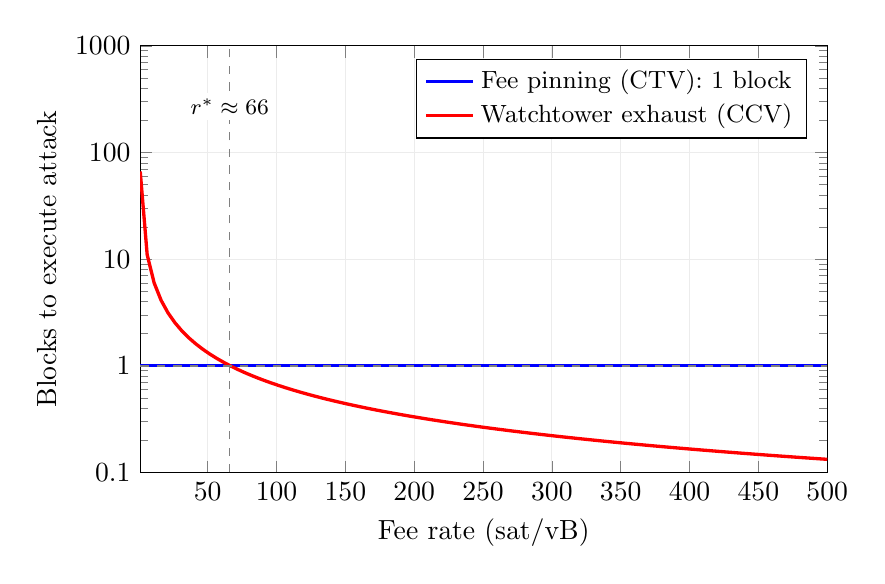
\begin{tikzpicture}
\begin{axis}[
  width=0.85\textwidth,
  height=7cm,
  xlabel={Fee rate (sat/vB)},
  ylabel={Blocks to execute attack},
  xmin=1, xmax=500,
  ymode=log,
  ymin=0.1, ymax=1000,
  legend pos=north east,
  legend style={font=\small},
  grid=major,
  grid style={gray!15},
  ytick={0.1,1,10,100,1000},
  yticklabels={0.1,1,10,100,\num{1000}},
]
% Fee pinning — always 1 block (broadcast 25 descendants, wait for CSV expiry)
\addplot[very thick, blue, domain=1:500] {1};
\addlegendentry{Fee pinning (CTV): 1 block}

% Watchtower exhaustion — CCV
% splits = V / (recover * r) = 50000000 / (122 * r)
% blocks = splits / splits_per_block = 50000000 / (122 * r * 6172)
\addplot[very thick, red, domain=1:500, samples=100]
  {50000000 / (122 * x * 6172)};
\addlegendentry{Watchtower exhaust (CCV)}

% Feasibility threshold — below 1 block = executable in single block
\draw[dashed, gray, thick] (axis cs:1,1) -- (axis cs:500,1);

% Crossover annotation — where CCV drops below ~10 blocks (practical)
\draw[dashed, gray] (axis cs:66,0.1) -- (axis cs:66,1000);
\node[font=\footnotesize, fill=white, inner sep=2pt, anchor=south]
  at (axis cs:66,200) {$r^* \approx 66$};

\end{axis}
\end{tikzpicture}
\caption{Fee-dependent security inversion. CTV fee pinning (blue) executes in
one block regardless of fee rate. CCV per-UTXO recovery-cost scaling (red) requires
progressively fewer blocks as fees rise, because each split creates a larger
dust threshold. Below ${\sim}50$~sat/vB, exhaustion requires hundreds of blocks
(infeasible). Above $r^* \approx 66$~sat/vB, exhaustion completes within a few
blocks, making it practical. The crossover defines where the safety ranking inverts.}
\label{fig:fee_inversion}
\end{figure}

% ======================================================================
\section{Class \classfee{}: Fee-Channel Pinning (TM1)} \label{se:fee_pinning}

Fee pinning exploits CTV's anchor-based fee management. The unvault transaction
includes an anchor output at \texttt{vout=1} (3{,}300~sats) to enable CPFP fee
bumping. An attacker with the hot key broadcasts the unvault, then immediately
constructs 25 low-fee descendant transactions spending the anchor output. Bitcoin
Core's mempool policy limits descendant chains to 25 transactions; once the limit
is reached, the watchtower's CPFP recovery transaction is rejected because it would
exceed the descendant count.

\begin{figure}[t]
\centering
\resizebox{0.95\textwidth}{!}{%
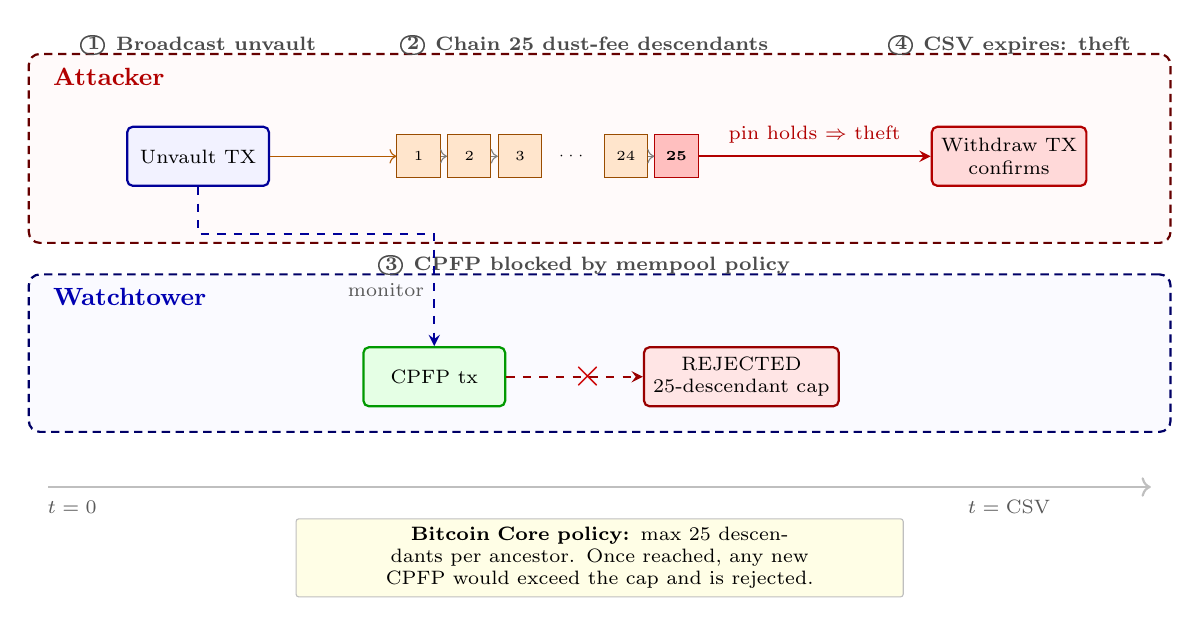
\begin{tikzpicture}[
  tx/.style={rectangle, draw, rounded corners=2pt, minimum width=1.8cm,
             minimum height=0.75cm, align=center, font=\scriptsize,
             fill=blue!5, draw=blue!60!black, thick},
  descendant/.style={rectangle, draw, minimum width=0.55cm, minimum height=0.55cm,
                     font=\tiny, fill=orange!20, draw=orange!60!black},
  wtx/.style={rectangle, draw, rounded corners=2pt, minimum width=1.8cm,
              minimum height=0.75cm, align=center, font=\scriptsize,
              fill=green!10, draw=green!60!black, thick},
  rej/.style={rectangle, draw, rounded corners=2pt, minimum width=2.2cm,
              minimum height=0.75cm, align=center, font=\scriptsize,
              fill=red!10, draw=red!60!black, thick},
  phase/.style={font=\scriptsize\bfseries, align=center, text=gray!60!black},
  note/.style={font=\scriptsize, align=center, text=gray!70!black},
  edge/.style={draw, ->, >=stealth, thick},
  lane/.style={rectangle, rounded corners=4pt, thick, dash pattern=on 3pt off 2pt},
]
  % ===== Top lane: attacker =====
  \node[lane, fill=red!2, draw=red!40!black, minimum width=14.5cm,
        minimum height=2.4cm] (alane) at (6.5, 2.0) {};
  \node[font=\small\bfseries, text=red!70!black, anchor=west]
       at ($(alane.north west)+(0.2,-0.3)$) {Attacker};

  % Phase 1
  \node[phase] at (1.4, 3.3) {\textcircled{\scriptsize 1} Broadcast unvault};
  \node[tx] (unvault) at (1.4, 1.9) {Unvault TX};

  % Phase 2: descendant chain
  \node[phase] at (6.3, 3.3) {\textcircled{\scriptsize 2} Chain 25 dust-fee descendants};
  \node[descendant] (d1) at (4.2, 1.9) {1};
  \node[descendant, right=0.08cm of d1] (d2) {2};
  \node[descendant, right=0.08cm of d2] (d3) {3};
  \node[font=\tiny, right=0.08cm of d3] (dots) {$\cdots$};
  \node[descendant, right=0.08cm of dots] (d24) {24};
  \node[descendant, right=0.08cm of d24, fill=red!25, draw=red!70!black] (d25) {\textbf{25}};
  \draw[->, thin, gray] (d1) -- (d2);
  \draw[->, thin, gray] (d2) -- (d3);
  \draw[->, thin, gray] (d24) -- (d25);
  \draw[->, thin, orange!70!black] (unvault.east) -- (d1.west);

  % Phase 4: withdrawal confirms (same lane)
  \node[phase] at (11.7, 3.3) {\textcircled{\scriptsize 4} CSV expires: theft};
  \node[tx, fill=red!15, draw=red!70!black] (theft) at (11.7, 1.9)
       {Withdraw TX\\ \scriptsize confirms};

  % ===== Bottom lane: watchtower =====
  \node[lane, fill=blue!2, draw=blue!40!black, minimum width=14.5cm,
        minimum height=2.0cm] (wlane) at (6.5, -0.6) {};
  \node[font=\small\bfseries, text=blue!70!black, anchor=west]
       at ($(wlane.north west)+(0.2,-0.3)$) {Watchtower};

  % Phase 3: CPFP rejected
  \node[phase] at (6.3, 0.5) {\textcircled{\scriptsize 3} CPFP blocked by mempool policy};
  \node[wtx] (cpfp) at (4.4, -0.9) {CPFP tx};
  \node[rej] (rejected) at (8.3, -0.9)
       {REJECTED\\ \scriptsize 25-descendant cap};
  \draw[edge, red!60!black, dashed] (cpfp.east) -- (rejected.west);
  \node[font=\Large, text=red!80!black] at (6.35, -0.9) {$\times$};

  % Monitor arrow (attacker -> watchtower)
  \draw[edge, dashed, blue!60!black] (unvault.south) -- ++(0,-0.6) -| (cpfp.north)
        node[pos=0.75, left, note] {monitor};

  % Theft consequence arrow (straight, same lane)
  \draw[edge, red!70!black, thick] (d25.east) -- (theft.west)
        node[midway, above=1pt, note, text=red!70!black] {pin holds $\Rightarrow$ theft};

  % ===== Timeline axis =====
  \draw[->, thick, gray!50] (-0.5, -2.3) -- (13.5, -2.3);
  \node[note, below=0.05cm of {(-0.2,-2.3)}] {$t = 0$};
  \node[note, below=0.05cm of {(11.7,-2.3)}] {$t = \text{CSV}$};

  % Annotation box
  \node[align=center, font=\scriptsize, fill=yellow!10, draw=gray!50,
        rounded corners=1pt, inner sep=3pt, text width=7.5cm]
       at (6.5, -3.2)
       {\textbf{Bitcoin Core policy:} max 25 descendants per ancestor.
        Once reached, any new CPFP would exceed the cap and is rejected.};

\end{tikzpicture}}
\caption{Fee pinning attack against CTV (\textbf{TM1}).
\textcircled{\scriptsize 1}~Attacker broadcasts the unvault, starting the CSV
window. \textcircled{\scriptsize 2}~Attacker chains 25 dust-rate descendants off
the anchor output, filling the mempool descendant limit.
\textcircled{\scriptsize 3}~The watchtower's CPFP recovery is rejected by mempool
policy (adding it would exceed the 25-descendant cap).
\textcircled{\scriptsize 4}~When CSV expires, the attacker's pre-committed
withdrawal confirms.}
\label{fig:fee_pinning}
\end{figure}

The attack cost function (Equation~\ref{eq:pin_cost}) evaluates to approximately
14{,}300~sats at dust-rate fees, regardless of the prevailing fee environment. At a
vault value of 0.5~BTC (50{,}000{,}000~sats), the attack costs 0.03\% of the vault
value---well below any economic rationality threshold.

CCV, OP\_VAULT, and CAT+CSFS are immune to this specific attack. CCV and OP\_VAULT
do not use anchor outputs (fees are paid via separate mechanisms). CAT+CSFS uses
\texttt{SIGHASH\_SINGLE|ANYONECANPAY}, which allows external fee inputs without
an anchor output.

\paragraph{Timing assumption.}
The attack requires the attacker to broadcast all 25 descendant transactions and
have them accepted into mempools \emph{before} the watchtower broadcasts its CPFP
recovery transaction. On mainnet, a well-configured watchtower would have its CPFP
transaction pre-constructed and ready to broadcast immediately upon detecting the
unvault. The attack therefore depends on a propagation race: the attacker must fill
the descendant chain across a sufficient fraction of the network's mempools before
the watchtower's single CPFP transaction propagates. Our regtest experiment
(Chapter~\ref{ch:results}) demonstrates that the descendant chain construction is
structurally valid---the 25-transaction chain is accepted and the CPFP is
rejected---but cannot test the propagation race, because regtest has a single
mempool with no network latency. The practical feasibility of this attack on mainnet
depends on the relative propagation speeds of the attacker's 25~transactions versus
the watchtower's single transaction, which is a network-layer question outside the
scope of this work (see Section~\ref{se:limitations} for further discussion).

TRUC/v3 transactions (merged in Bitcoin Core 28.0) limit descendant chains to a
single transaction. If CTV vault transactions opt into TRUC, the 25-descendant
pinning vector is eliminated at the relay policy level, potentially changing the
crossover result of Proposition~\ref{thm:fee_inversion}.

% ======================================================================
\section{Class \classscale{}: Per-UTXO Recovery-Cost Scaling (TM4)} \label{se:watchtower_exhaustion}

CCV and OP\_VAULT support partial withdrawals via \texttt{trigger\_and\_revault},
which splits the vault into a withdrawal portion and a re-locked remainder. An
attacker with the trigger key can repeatedly invoke this operation, splitting the
vault into progressively smaller UTXOs. When individual UTXOs become small enough
that the recovery transaction fee exceeds the UTXO value, those funds are
effectively lost---the watchtower cannot economically justify recovering them.

\begin{figure}[t]
\centering
\resizebox{0.95\textwidth}{!}{%
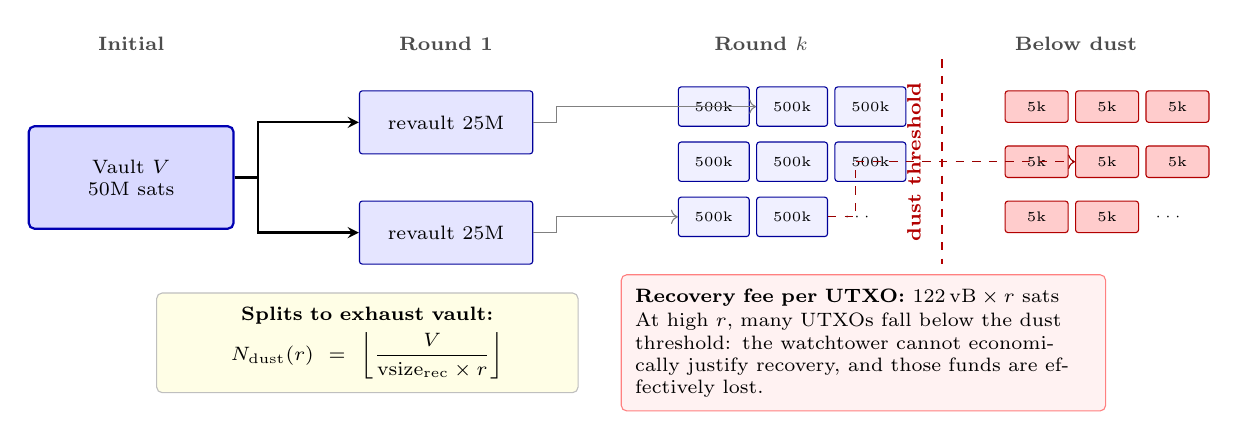
\begin{tikzpicture}[
  vault/.style={rectangle, draw, rounded corners=2pt, align=center,
                font=\scriptsize, fill=blue!15, draw=blue!70!black, thick},
  mid/.style={rectangle, draw, rounded corners=1pt, align=center,
              font=\scriptsize, fill=blue!10, draw=blue!60!black},
  small/.style={rectangle, draw, rounded corners=1pt, align=center,
                font=\tiny, fill=blue!6, draw=blue!60!black,
                minimum width=0.9cm, minimum height=0.5cm},
  dust/.style={rectangle, draw, rounded corners=1pt, align=center,
               font=\tiny, fill=red!20, draw=red!70!black,
               minimum width=0.8cm, minimum height=0.4cm},
  phase/.style={font=\scriptsize\bfseries, text=gray!60!black, align=center},
  note/.style={font=\scriptsize, align=center, text=gray!70!black},
  edge/.style={draw, ->, >=stealth, thick},
]
  % Phase headers
  \node[phase] at (0, 3.2)   {Initial};
  \node[phase] at (4.0, 3.2) {Round 1};
  \node[phase] at (8.0, 3.2) {Round $k$};
  \node[phase] at (12.0, 3.2) {Below dust};

  % Initial vault
  \node[vault, minimum width=2.6cm, minimum height=1.3cm] (v0) at (0, 1.5)
       {Vault $V$\\ 50M sats};

  % Round 1: two halves
  \node[mid, minimum width=2.2cm, minimum height=0.8cm] (v1a) at (4.0, 2.2)
       {revault 25M};
  \node[mid, minimum width=2.2cm, minimum height=0.8cm] (v1b) at (4.0, 0.8)
       {revault 25M};
  \draw[edge] (v0.east) -- ++(0.3,0) |- (v1a.west);
  \draw[edge] (v0.east) -- ++(0.3,0) |- (v1b.west);

  % Round k: many small UTXOs (shown as grid)
  \node[small] (s1) at (7.4, 2.4) {500k};
  \node[small, right=0.08cm of s1] (s2) {500k};
  \node[small, right=0.08cm of s2] (s3) {500k};
  \node[small] (s4) at (7.4, 1.7) {500k};
  \node[small, right=0.08cm of s4] (s5) {500k};
  \node[small, right=0.08cm of s5] (s6) {500k};
  \node[small] (s7) at (7.4, 1.0) {500k};
  \node[small, right=0.08cm of s7] (s8) {500k};
  \node[font=\tiny, right=0.08cm of s8] {$\cdots$};
  \draw[->, thin, gray] (v1a.east) -- ++(0.3,0) |- (s2.west);
  \draw[->, thin, gray] (v1b.east) -- ++(0.3,0) |- (s7.west);

  % Below dust
  \node[dust] (d1) at (11.5, 2.4) {5k};
  \node[dust, right=0.08cm of d1] (d2) {5k};
  \node[dust, right=0.08cm of d2] (d3) {5k};
  \node[dust] (d4) at (11.5, 1.7) {5k};
  \node[dust, right=0.08cm of d4] (d5) {5k};
  \node[dust, right=0.08cm of d5] (d6) {5k};
  \node[dust] (d7) at (11.5, 1.0) {5k};
  \node[dust, right=0.08cm of d7] (d8) {5k};
  \node[font=\tiny, right=0.08cm of d8] {$\cdots$};
  \draw[->, thin, red!60!black, dashed] (s8.east) -- ++(0.35,0) |- (d5.west);

  % Dust threshold bar (ABOVE the dust row, not cutting through others)
  \draw[red!70!black, thick, dashed] (10.3, 3.0) -- (10.3, 0.4);
  \node[font=\scriptsize\bfseries, text=red!70!black, rotate=90, anchor=south]
        at (10.15, 1.7) {dust threshold};

  % Bottom: formula and explanation
  \node[align=center, font=\scriptsize, fill=yellow!10, draw=gray!50,
        rounded corners=2pt, inner sep=5pt, text width=5cm] at (3.0, -0.6)
       {\textbf{Splits to exhaust vault:}\\[2pt]
        $N_{\text{dust}}(r) =
         \left\lfloor \dfrac{V}{\text{vsize}_{\text{rec}} \times r} \right\rfloor$};

  \node[align=left, font=\scriptsize, fill=red!5, draw=red!50,
        rounded corners=2pt, inner sep=5pt, text width=5.8cm]
        at (9.3, -0.6)
       {\textbf{Recovery fee per UTXO:} $122\vB \times r$ sats\\[1pt]
        At high $r$, many UTXOs fall below the dust threshold:
        the watchtower cannot economically justify recovery,
        and those funds are effectively lost.};

\end{tikzpicture}}
\caption{Watchtower exhaustion via \texttt{trigger\_and\_revault} (\textbf{TM4}).
The attacker (holding the trigger key) repeatedly splits the vault into smaller
UTXOs. As UTXOs shrink, the per-recovery fee ($\text{vsize}_{\text{rec}} \times r$)
consumes an increasing fraction of each UTXO's value. Once a UTXO's value falls
below $\text{vsize}_{\text{rec}} \times r$, the watchtower cannot economically
justify recovery---those funds are effectively lost.}
\label{fig:watchtower_exhaustion}
\end{figure}

Using the measured transaction sizes from Chapter~\ref{ch:results}, we compute the
splitting capacity per block. Each \texttt{trigger\_and\_revault} transaction weighs
approximately 648~WU for CCV and 1{,}168~WU for OP\_VAULT. The maximum block weight
is 4{,}000{,}000~WU, yielding:

\begin{align}
\text{CCV splits/block}      &\approx \frac{4{,}000{,}000}{648} \approx 6{,}172 \\
\text{OP\_VAULT splits/block} &\approx \frac{4{,}000{,}000}{1{,}168} \approx 3{,}427
\end{align}

Harding~\cite{Har24} estimated approximately 3{,}000 splits per block based on
assumed OP\_VAULT-sized transactions. Our measurement confirms this for OP\_VAULT
(3{,}427, within 14\% of the estimate) but reveals that CCV achieves approximately
80\% more splits per block due to its smaller trigger transaction (162\vB{} vs.\
292\vB{}). This correction matters because CCV (BIP-443) is the active proposal
that replaced OP\_VAULT (BIP-345): the design that Bitcoin is most likely to adopt
has a larger per-UTXO recovery-cost scaling surface than previously estimated.

The watchtower's recovery budget determines how many splits it can absorb. At
fee rate~$r$, recovering a single split costs $\text{vsize}_{\text{recover}} \times r$
sats (122$r$ for CCV, 246$r$ for OP\_VAULT). The total recovery budget needed to
defend against $N$ splits is $N \times \text{vsize}_{\text{recover}} \times r$.
For a 0.5~BTC vault at 100\satvB{}, defending against 1{,}000 splits costs
$1{,}000 \times 122 \times 100 = 12{,}200{,}000$~sats (0.122~BTC)---roughly 24\%
of the vault value.

\subsection{Batched Defender Strategy}
\label{ss:batched_defender}

The analysis above assumes single-input recovery: one transaction per
recovered Unvaulting UTXO. BIP-345's ``Batching'' section (authorized
recovery, lines 613--621) and BIP-443's default aggregation mode both
permit the defender to recover $N$ UTXOs in a single transaction, with
vsize scaling as $\alpha + \beta \cdot N$ where $\alpha$ is fixed
overhead and $\beta$ is the marginal per-input cost. We measure both
constants empirically on regtest, sweeping $N \in \{2, 5, 10, 25, 50\}$
and extracting $(\alpha, \beta)$ by linear regression:

\begin{table}[h]
\centering
\caption{Measured batched-recovery constants on regtest. The fit
$\text{vsize}(N) = \alpha + \beta \cdot N$ replaces the single-input
$\text{vsize}_{\text{recover}}$ with an amortized per-UTXO cost
$\alpha/N + \beta \to \beta$ for large $N$.}
\label{tab:batched_recovery}
\begin{tabular}{@{}lccccc@{}}
\toprule
Design     & $\alpha$ (\vB) & $\beta$ (\vB) & Unbatched $r^\dagger$ & Batched $r^\dagger$ & Factor \\
\midrule
CCV        & 54  & 68 & 66\satvB  & 119\satvB & $1.8\times$ \\
OP\_VAULT  & 154 & 92 & 59\satvB  & 159\satvB & $2.7\times$ \\
\bottomrule
\end{tabular}
\end{table}

Substituting $\beta$ for $\text{vsize}_{\text{recover}}$ in
Equation~\ref{eq:r_star} yields the batched dust-threshold
$r^\dagger_{\text{batched}}(V, D) = V / (\beta(D) \times S(D))$. For
a 0.5~BTC vault the batched thresholds rise to 119\satvB{} for CCV and
159\satvB{} for OP\_VAULT---roughly $1.8\times$ and $2.7\times$ the
unbatched values. The larger multiplier for OP\_VAULT reflects its
larger unbatched recovery transaction (246\vB{}): batching amortizes
that overhead more aggressively than CCV's already-small 122\vB{}
recovery.

\paragraph{Batching flips the TM4 ordering.}
Unbatched, CCV is safer than OP\_VAULT against per-UTXO recovery-cost scaling
($r^\dagger$ 66 vs 59). Once the defender batches, the ordering flips:
OP\_VAULT becomes safer ($r^\dagger$ 159 vs 119). The intuition is that
CCV's lead under single-input recovery comes from a smaller
$\text{vsize}_{\text{recover}}$, but under batching the relevant cost
is the marginal per-input $\beta$, which is nearly equal across the
two designs (68 vs 92\vB). OP\_VAULT's lower splits-per-block
($S = 3{,}427$ vs $6{,}172$) then dominates, yielding the higher
$r^\dagger$. The operational implication is that the
``CCV has a larger per-UTXO recovery-cost scaling surface'' conclusion of the
unbatched analysis reverses once watchtower operators adopt batched
recovery---a non-trivial finding for vault designers choosing between
BIP-443 and BIP-345.

\paragraph{Constraints on batched recovery.}
BIP-345's authorized recovery permits batching across vaults with
distinct \texttt{<recovery-sPK-hash>} values (§``Batching'' lines
618--621), allowing a single watchtower to serve multiple independent
users in one transaction. Unauthorized recovery is capped at two
outputs (lines 389--391) and thus limited to same-\texttt{recovery-sPK}
batches. BIP-443's default aggregation has no taptree-equivalence
requirement and is strictly more permissive. The attacker's
\texttt{trigger\_and\_revault} sequence is inherently serial---each
revault consumes the previous output---so the attacker does not
benefit from batching. The measured savings accrue asymmetrically to
the defender.

CTV, CAT+CSFS, and Simplicity are immune to per-UTXO recovery-cost scaling because they do
not support partial withdrawals. The entire vault balance must be unvaulted
atomically, so the watchtower needs only one recovery transaction regardless of
attack persistence.

% ======================================================================
\section{Class \classgrief{}: Permissionless Griefing (TM2)} \label{se:recovery_griefing}

Recovery griefing is a denial-of-service attack where the adversary repeatedly
invokes recovery to prevent the vault owner from completing withdrawals. The
economic asymmetry between attacker and defender costs determines the severity.

\begin{figure}[t]
\centering
\resizebox{0.9\textwidth}{!}{%
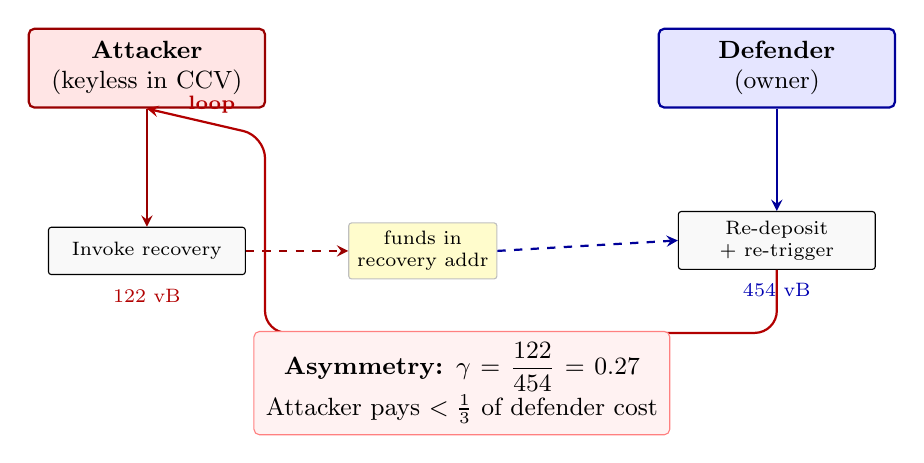
\begin{tikzpicture}[
  node distance=1.0cm,
  actor/.style={rectangle, draw, rounded corners=2pt, minimum width=3.0cm,
                minimum height=1.0cm, align=center, font=\small,
                thick},
  attacker/.style={actor, fill=red!10, draw=red!60!black},
  defender/.style={actor, fill=blue!10, draw=blue!60!black},
  action/.style={rectangle, draw, rounded corners=1pt, minimum width=2.5cm,
                 minimum height=0.6cm, align=center, font=\scriptsize,
                 fill=gray!5},
  cost/.style={font=\scriptsize, text=red!70!black, align=center},
  note/.style={font=\scriptsize, align=center, text=gray!70!black},
  edge/.style={draw, ->, >=stealth, thick},
]
  % Attacker side
  \node[attacker] (att) at (0, 0) {\textbf{Attacker}\\ (keyless in CCV)};

  % Defender side
  \node[defender] (def) at (8, 0) {\textbf{Defender}\\ (owner)};

  % Action 1: attacker invokes recovery
  \node[action, below=1.5cm of att] (act1) {Invoke recovery};
  \node[cost, below=0.05cm of act1] (c1) {122 vB};
  \draw[edge, red!60!black] (att.south) -- (act1.north);

  % Fund state 1
  \node[font=\scriptsize, align=center, fill=yellow!20, draw=gray!50,
        rounded corners=1pt, right=1.3cm of act1, inner sep=3pt, minimum height=0.7cm]
       (s1) {funds in\\ recovery addr};

  % Action 2: defender re-deposits + re-triggers
  \node[action, below=1.3cm of def] (act2) {Re-deposit\\ + re-trigger};
  \node[cost, below=0.05cm of act2, text=blue!70!black] (c2) {454 vB};
  \draw[edge, blue!60!black] (def.south) -- (act2.north);

  % Loop arrow
  \draw[edge, red!60!black, dashed] (act1.east) -- (s1.west);
  \draw[edge, blue!60!black, dashed] (s1.east) -- (act2.west);
  \draw[edge, red!70!black, thick, rounded corners=8pt]
       (act2.south) -- ++(0,-0.8) -- ++(-6.5,0) -- ++(0,2.5) -- (att.south)
       node[midway, above, note, text=red!70!black, pos=0.45] {\textbf{loop}};

  % Asymmetry indicator
  \node[align=center, font=\small, text width=5cm, fill=red!5,
        draw=red!50, rounded corners=2pt, inner sep=4pt]
       at (4, -4) {\textbf{Asymmetry:} $\gamma = \dfrac{122}{454} = 0.27$\\
                  Attacker pays $<\tfrac{1}{3}$ of defender cost};

\end{tikzpicture}}
\caption{Recovery griefing loop (\textbf{TM2}) for CCV. The attacker triggers
permissionless recovery (122\vB{}); the owner must re-deposit and re-trigger
(454\vB{}) to resume withdrawal; the attacker invokes recovery again. The
per-round cost asymmetry $\gamma = 0.27$ strongly favors the attacker.}
\label{fig:recovery_griefing}
\end{figure}

Table~\ref{tab:griefing_costs} compares the per-round costs. The griefing ratio
$\gamma = \text{vsize}_{\text{attack}} / \text{vsize}_{\text{defend}}$ measures the
cost asymmetry: $\gamma < 1$ means the attacker pays less than the defender per
round (favorable to the attacker).

\begin{equation} \label{eq:griefing_ratio}
\gamma = \frac{\text{vsize}_{\text{attack}}}{\text{vsize}_{\text{defend}}}
\end{equation}

\begin{table}[t]
\centering
\caption{Recovery griefing cost comparison. The attacker invokes recovery; the
defender re-deposits and re-triggers. $\gamma < 1$ favors the attacker.}
\label{tab:griefing_costs}
\small
\begin{tabular}{@{}llrrrl@{}}
\toprule
Covenant & Key required & Attacker & Defender & $\gamma$ & Assessment \\
         &              & (vB/round) & (vB/round) & & \\
\midrule
CCV       & None (keyless)  & 122 & 454 & 0.27 & Severe (anyone) \\
OP\_VAULT & recoveryauth    & 246 & 446 & 0.55 & Low (key needed) \\
CTV       & Hot key         & 94  & 133 & 0.71 & Moderate (reversed) \\
CAT+CSFS  & Cold key        & 125 & 343 & 0.36 & Irrelevant (TM11) \\
\bottomrule
\end{tabular}
\end{table}

CCV has the most severe griefing profile: the attack is keyless (anyone can invoke
recovery) and the cost asymmetry strongly favors the attacker ($\gamma = 0.27$).
OP\_VAULT eliminates anonymous griefing by requiring the \texttt{recoveryauth} key,
raising the attacker bar substantially. CTV's griefing direction is reversed: the
attacker triggers an unvault (94\vB{}) and the defender sweeps to cold (133\vB{}).
CAT+CSFS griefing requires the cold key, but cold key compromise already constitutes
total fund theft (TM11), making the griefing scenario academically moot.

% ======================================================================
\section{Class \classhot{}: Hot-Key Theft via Destination Substitution (TM3)} \label{se:trigger_theft}

Trigger key compromise has different consequences across designs because the vault's
output constraints determine what the attacker can do with the triggered funds.

\begin{figure}[t]
\centering
\resizebox{0.95\textwidth}{!}{%
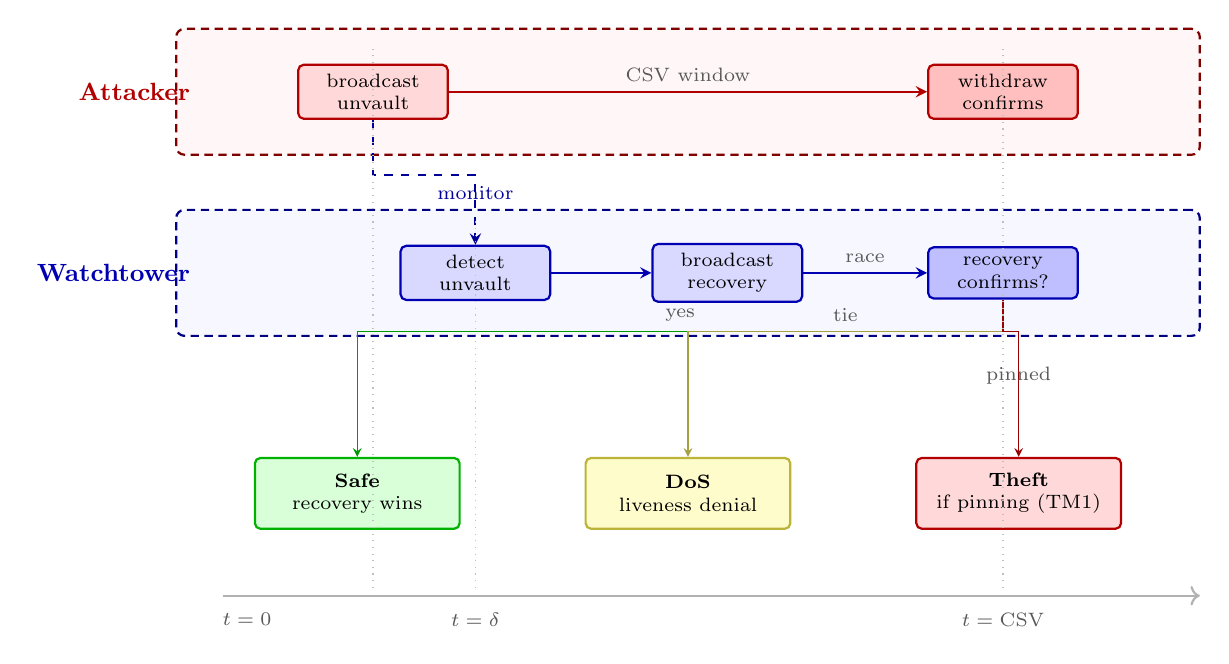
\begin{tikzpicture}[
  lane/.style={rectangle, draw, thick, minimum width=13cm, minimum height=1.6cm,
               rounded corners=3pt, dash pattern=on 3pt off 2pt},
  action/.style={rectangle, draw, rounded corners=2pt, minimum width=1.9cm,
                 minimum height=0.65cm, align=center, font=\scriptsize, thick},
  actatk/.style={action, fill=red!15, draw=red!70!black},
  actdef/.style={action, fill=blue!15, draw=blue!70!black},
  outcome/.style={rectangle, draw, rounded corners=2pt, minimum width=2.6cm,
                  minimum height=0.9cm, align=center, font=\scriptsize, thick},
  note/.style={font=\scriptsize, align=center, text=gray!70!black},
  tlabel/.style={font=\scriptsize, text=gray!70!black, anchor=north},
  edge/.style={draw, ->, >=stealth, thick},
]
  % ===== Attacker lane =====
  \node[lane, fill=red!3, draw=red!50!black] (alane) at (6.5, 3.0) {};
  \node[font=\small\bfseries, text=red!70!black, anchor=east] at (0.3, 3.0) {Attacker};

  \node[actatk] (au) at (2.5, 3.0) {broadcast\\ unvault};
  \node[actatk, fill=red!25] (aw) at (10.5, 3.0) {withdraw\\ confirms};
  \draw[edge, red!70!black] (au.east) -- (aw.west)
        node[midway, above, note] {CSV window};

  % ===== Watchtower lane =====
  \node[lane, fill=blue!3, draw=blue!50!black] (wlane) at (6.5, 0.7) {};
  \node[font=\small\bfseries, text=blue!70!black, anchor=east] at (0.3, 0.7) {Watchtower};

  \node[actdef] (wd) at (3.8, 0.7) {detect\\ unvault};
  \node[actdef] (wb) at (7.0, 0.7) {broadcast\\ recovery};
  \node[actdef, fill=blue!25] (wc) at (10.5, 0.7) {recovery\\ confirms?};
  \draw[edge, blue!70!black] (wd.east) -- (wb.west);
  \draw[edge, blue!70!black] (wb.east) -- (wc.west)
        node[midway, above, note] {race};

  % Monitor arrow (attacker -> watchtower) — routed to avoid overlap
  \draw[edge, dashed, blue!60!black] (au.south) -- ++(0, -0.7) -| (wd.north)
        node[pos=0.75, above, note, text=blue!60!black] {monitor};

  % ===== Outcomes row (below watchtower) =====
  \node[outcome, fill=green!15, draw=green!70!black] (safe) at (2.3, -2.1)
       {\textbf{Safe}\\ recovery wins};
  \node[outcome, fill=yellow!20, draw=yellow!70!black] (dos) at (6.5, -2.1)
       {\textbf{DoS}\\ liveness denial};
  \node[outcome, fill=red!15, draw=red!70!black] (theft) at (10.7, -2.1)
       {\textbf{Theft}\\ if pinning (TM1)};

  % Connect "recovery confirms?" to outcomes — fan-out with labels
  \draw[edge, thin, green!60!black] (wc.south) -- ++(0, -0.4) -| (safe.north)
        node[pos=0.25, above, note] {yes};
  \draw[edge, thin, yellow!60!black] (wc.south) -- ++(0, -0.4) -| (dos.north)
        node[pos=0.25, above, note] {tie};
  \draw[edge, thin, red!60!black] (wc.south) -- ++(0, -0.4) -| (theft.north)
        node[pos=0.75, above, note] {pinned};

  % ===== Timeline axis =====
  \draw[->, thick, gray!60] (0.6, -3.4) -- (13.0, -3.4);
  \node[tlabel] at (0.9, -3.5) {$t = 0$};
  \node[tlabel] at (3.8, -3.5) {$t = \delta$};
  \node[tlabel] at (10.5, -3.5) {$t = \text{CSV}$};

  % Vertical event guides (subtle)
  \draw[dotted, gray!50] (2.5, -3.3) -- (2.5, 3.55);
  \draw[dotted, gray!50] (3.8, -3.3) -- (3.8, 1.4);
  \draw[dotted, gray!50] (10.5, -3.3) -- (10.5, 3.55);

\end{tikzpicture}}
\caption{Trigger key theft race (\textbf{TM3}). The attacker broadcasts an
unvault (upper lane). The watchtower detects it at time $\delta$ and broadcasts
recovery (lower lane). The outcome hinges on whether recovery confirms before
CSV expiry: safe if recovery wins, DoS if tied, theft if the attacker successfully
pins the watchtower's transaction (combining TM3 with TM1).}
\label{fig:trigger_theft}
\end{figure}

\paragraph{CTV.} The hot key can trigger the unvault transaction and, after the CSV
delay, complete the withdrawal to the pre-committed destination. If the attacker also
holds the fee key (enabling fee pinning to block recovery), this escalates to fund
theft. Hot key alone produces liveness denial only---the defender sweeps to cold
storage.

\paragraph{CCV.} The trigger key can direct the withdrawal to an attacker-controlled
address (the destination is chosen at trigger time, not fixed at creation). The
watchtower races to invoke keyless recovery (122\vB{}). Since recovery is
permissionless, the watchtower needs no additional key material to respond.

\paragraph{OP\_VAULT.} The trigger key can redirect withdrawals, similar to CCV. The
watchtower races to invoke authorized recovery (246\vB{}), which requires the
\texttt{recoveryauth} key. If the attacker compromises both the trigger key and the
recoveryauth key, the result is persistent liveness denial (not theft), because the
recovery address is pre-committed in the vault's Taproot internal key tweak and cannot
be changed.

\paragraph{CAT+CSFS.} The hot key can only trigger to the pre-committed vault-loop
output. The dual CSFS+CHECKSIG verification binds the output to the embedded
\texttt{sha\_single\_output} constant---changing the output changes the sighash,
invalidating the signature. The hot key holder is limited to griefing (triggering
unwanted unvaults that the defender can recover from). This is the strongest hot-key
theft resistance of any design studied.

% ======================================================================
\section{Class \classcold{}: Cold-Key Theft via Unconstrained Recovery (TM11)} \label{se:cold_key_recovery}

Cold key compromise has asymmetric consequences depending on whether the recovery
path constrains outputs.

\begin{figure}[t]
\centering
\resizebox{0.95\textwidth}{!}{%
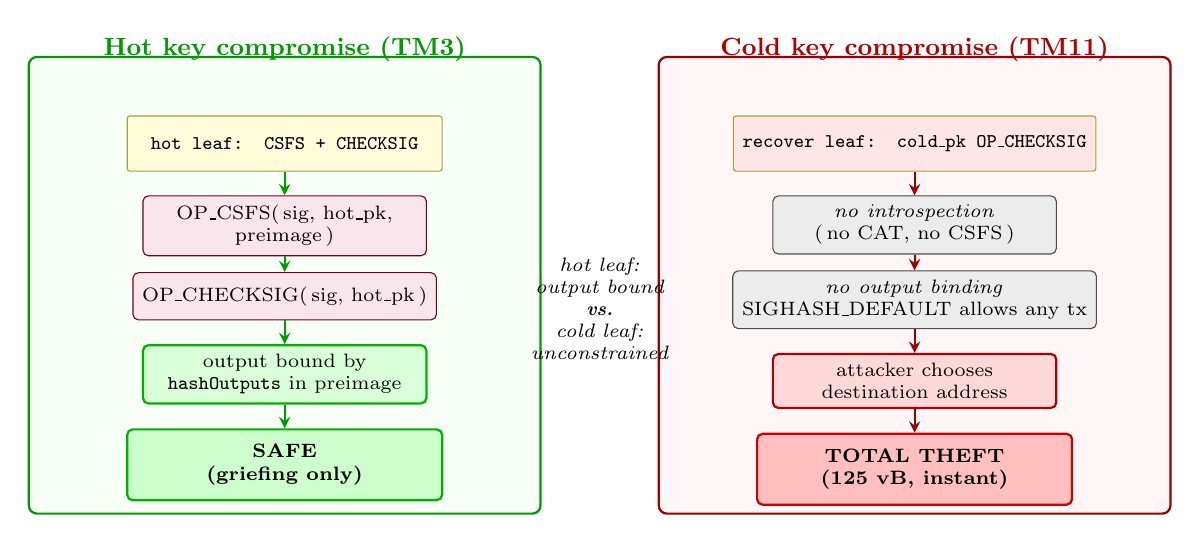
\begin{tikzpicture}[
  node distance=0.8cm,
  scenario/.style={rectangle, draw, rounded corners=3pt, thick,
                   minimum width=6.5cm, minimum height=5.8cm},
  hot/.style={scenario, fill=green!3, draw=green!60!black},
  cold/.style={scenario, fill=red!3, draw=red!60!black},
  leaf/.style={rectangle, draw, rounded corners=1pt, align=center,
               font=\scriptsize\ttfamily, minimum width=4.0cm,
               minimum height=0.7cm, fill=yellow!15, draw=yellow!60!black},
  op/.style={rectangle, draw, rounded corners=2pt, align=center,
             font=\scriptsize, minimum width=3.6cm, minimum height=0.6cm,
             fill=purple!10, draw=purple!60!black},
  bad/.style={rectangle, draw, rounded corners=2pt, align=center, thick,
              font=\scriptsize, minimum width=3.6cm, minimum height=0.6cm,
              fill=red!15, draw=red!70!black},
  good/.style={rectangle, draw, rounded corners=2pt, align=center, thick,
               font=\scriptsize, minimum width=3.6cm, minimum height=0.6cm,
               fill=green!15, draw=green!70!black},
  outcome/.style={rectangle, draw, rounded corners=2pt, align=center,
                  font=\scriptsize\bfseries, minimum width=4.0cm,
                  minimum height=0.9cm, thick},
  note/.style={font=\scriptsize, align=center, text=gray!70!black},
  edge/.style={draw, ->, >=stealth, thick},
]
  % LEFT SCENARIO: hot key compromise (safe)
  \node[hot] (hotbox) at (-4, 0) {};
  \node[font=\small\bfseries, text=green!60!black, above=-0.2cm of hotbox.north]
       {Hot key compromise (TM3)};
  \node[leaf] at (-4, 1.8) (hleaf) {hot leaf: CSFS + CHECKSIG};
  \node[op, below=0.3cm of hleaf] (csfs1) {OP\_CSFS(\,sig, hot\_pk,\\
        \scriptsize preimage\,)};
  \node[op, below=0.2cm of csfs1] (csig1) {OP\_CHECKSIG(\,sig, hot\_pk\,)};
  \node[good, below=0.3cm of csig1] (bind)
       {output bound by\\ \texttt{hashOutputs} in preimage};
  \node[outcome, below=0.3cm of bind, fill=green!20, draw=green!70!black]
       (safe) {SAFE\\ (griefing only)};

  % RIGHT SCENARIO: cold key compromise (total theft)
  \node[cold] (coldbox) at (4, 0) {};
  \node[font=\small\bfseries, text=red!70!black, above=-0.2cm of coldbox.north]
       {Cold key compromise (TM11)};
  \node[leaf, fill=red!10] at (4, 1.8) (cleaf) {recover leaf: cold\_pk OP\_CHECKSIG};
  \node[op, below=0.3cm of cleaf, fill=gray!15, draw=gray!60!black]
       (none) {\textit{no introspection}\\
              \scriptsize (\,no CAT, no CSFS\,)};
  \node[op, below=0.2cm of none, fill=gray!15, draw=gray!60!black]
       (nobind) {\textit{no output binding}\\ \scriptsize
                 SIGHASH\_DEFAULT allows any tx};
  \node[bad, below=0.3cm of nobind]
       (sweep) {attacker chooses\\ destination address};
  \node[outcome, below=0.3cm of sweep, fill=red!25, draw=red!80!black]
       (theft) {\textbf{TOTAL THEFT}\\ (125 vB, instant)};

  % Edges inside each box
  \draw[edge, green!60!black] (hleaf) -- (csfs1);
  \draw[edge, green!60!black] (csfs1) -- (csig1);
  \draw[edge, green!60!black] (csig1) -- (bind);
  \draw[edge, green!60!black] (bind) -- (safe);

  \draw[edge, red!60!black] (cleaf) -- (none);
  \draw[edge, red!60!black] (none) -- (nobind);
  \draw[edge, red!60!black] (nobind) -- (sweep);
  \draw[edge, red!60!black] (sweep) -- (theft);

  % Central contrast annotation
  \node[align=center, font=\scriptsize\itshape, text width=2.5cm]
       at (0, -0.3) {hot leaf:\\ output bound\\ \textbf{vs.}\\
                     cold leaf:\\ unconstrained};

\end{tikzpicture}}
\caption{CAT+CSFS asymmetric key safety. \textbf{Left:} hot key compromise leaks
only the trigger authority---the dual CSFS$\,+\,$CHECKSIG binding forces outputs
to match the embedded \texttt{sha\_single\_output} constant (\textbf{TM3} reduces
to griefing). \textbf{Right:} cold key compromise yields total theft (\textbf{TM11}):
the recovery leaf is bare \texttt{OP\_CHECKSIG}---no timelock, no introspection,
no destination constraint. The attacker sweeps funds to any address in one 125\vB{}
transaction.}
\label{fig:cold_key_theft}
\end{figure}

\paragraph{CAT+CSFS.} The recovery leaf is \texttt{cold\_pk
OP\_CHECKSIG} with \sighash{DEFAULT}: no introspection, no
timelock, no output constraint. Cold key compromise grants
immediate, unrestricted theft---the attacker sends all funds to an
arbitrary address in a 125\vB{} transaction indistinguishable from
legitimate recovery on-chain. Of the four designs, this is the
worst-case TM11 profile.

\paragraph{CTV.} The cold sweep is CTV-committed, sending funds to the pre-committed
cold address. Cold key compromise allows forced recovery but only to that address.
The attacker cannot redirect funds.

\paragraph{OP\_VAULT.} Recovery is output-constrained to the pre-committed recovery
address (embedded in the Taproot internal key tweak). Cold key compromise plus
recoveryauth key compromise yields persistent denial of service but not theft.

\paragraph{CCV.} Recovery is keyless and output-constrained. There is no cold key to
compromise in the recovery path.

\paragraph{Simplicity.} Both trigger and recovery enforce
\texttt{jet::outputs\_hash()}, constraining recovery to the pre-committed address.
Cold key compromise forces recovery but cannot redirect funds---matching CCV and
OP\_VAULT's output-constrained model.

The recovery safety ranking is: CCV (keyless, constrained) $>$ OP\_VAULT
(key-gated, constrained) $>$ CTV (key-gated, constrained) $>$ CAT+CSFS
(key-gated, \emph{unconstrained}). Poelstra~\cite{Poe21} proposed an alternative
CAT+CSFS recovery design using recursive staging resets, where cold key compromise
leads to a liveness battle rather than immediate theft. Under that design, the
attacker and owner take turns resetting the vault state, each paying transaction fees
per round. This would upgrade CAT+CSFS's recovery safety to match OP\_VAULT's
(liveness denial, not theft), but at the cost of a larger recovery script and
additional witness overhead.

% ======================================================================
\section{Projection onto the $(g, b)$ Sublattice} \label{se:two_dim}

The design-space decomposition of Section~\ref{ss:design_space} induces
a natural projection onto the $(g, b)$ sublattice---the two recovery-path
dimensions---whose structure captures the recovery-related tradeoffs
without appeal to per-design measurement.

\begin{lemma}\label{lem:projection}
Let $D = (f, a, g, b)$ be a design with uniform leaf binding (hot and
cold paths share the same~$b$). Then:
\begin{enumerate}
  \item As $g$ weakens from $g_{\text{key}}$ to $g_{\text{keyless}}$,
    $\mathcal{L}(\mathrm{TM2})$ increases by
    Lemma~\ref{lem:keyless_grief}, while the key-loss attack surface
    vanishes.
  \item As $b$ weakens from $b_{\text{bound}}$ to $b_{\text{unbound}}$,
    $\mathcal{L}(\mathrm{TM11})$ increases from $0$ to $V$ by
    Lemma~\ref{lem:unbound_theft}.
  \item The cell $(g_{\text{keyless}}, b_{\text{unbound}})$ is
    unreachable: under Proposition~\ref{thm:griefing_safety}, a
    keyless vault with unbound recovery admits any party to invoke
    recovery to any destination, which is vacuous as a custody
    construction. No proposed BIP occupies this cell.
\end{enumerate}
\end{lemma}

\begin{proof}
Parts~1 and~2 are direct reinstatements of
Lemmas~\ref{lem:keyless_grief} and~\ref{lem:unbound_theft} with the $g$
and $b$ axes read individually. Part~3: if $\mathcal{A}(\emptyset) = 1$
and the recovery output is attacker-chooseable, any third party can
sweep the vault to their own address, reducing the construction to a
fee-free taproot \texttt{OP\_CHECKSIG} on a keyed path with no custody
benefit. \qed
\end{proof}

\begin{remark}\label{rem:asymmetric_binding}
Designs with \emph{asymmetric} leaf binding---hot leaf output-bound
and cold leaf unbound, as in CAT+CSFS---occupy two distinct cells in
this projection, one per leaf. The hot leaf sits at
$(g_{\text{key}}, b_{\text{bound}})$; the cold leaf sits at
$(g_{\text{key}}, b_{\text{unbound}})$. The ``off-axis'' position of
CAT+CSFS in a naive scatter visualisation is a direct consequence of
this leaf-level asymmetry, not an anomaly requiring a separate axis.
\end{remark}

\begin{figure}[t]
\centering
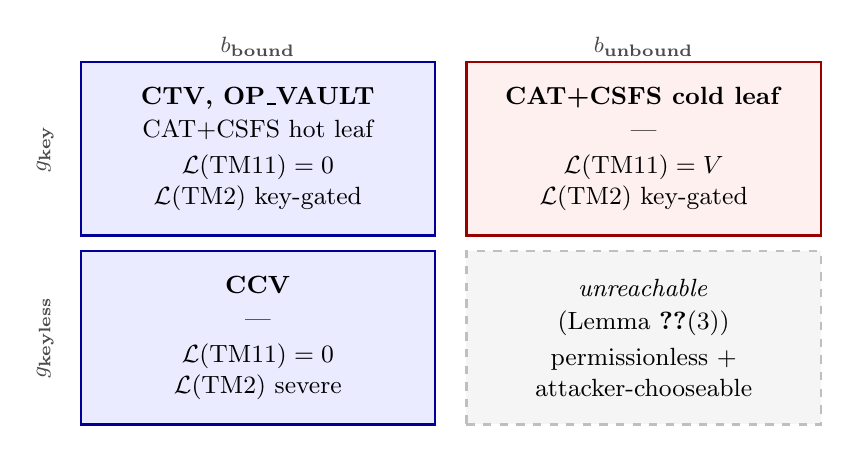
\begin{tikzpicture}[
  cell/.style={rectangle, draw, thick, minimum width=4.5cm,
               minimum height=2.2cm, align=center, font=\small},
  filled/.style={cell, fill=blue!8, draw=blue!60!black},
  asym/.style={cell, fill=red!6, draw=red!60!black},
  empty/.style={cell, fill=gray!8, draw=gray!50, dashed},
  axlbl/.style={font=\footnotesize\bfseries, text=gray!60!black,
                align=center},
]
  \node[axlbl] at (-0.5, 3.3) {$b_{\text{bound}}$};
  \node[axlbl] at (4.4, 3.3) {$b_{\text{unbound}}$};
  \node[axlbl, rotate=90] at (-3.2, 2.0) {$g_{\text{key}}$};
  \node[axlbl, rotate=90] at (-3.2, -0.4) {$g_{\text{keyless}}$};

  \node[filled] at (-0.5, 2.0) {\textbf{CTV, OP\_VAULT}\\[1pt]
        CAT+CSFS hot leaf\\[2pt]
        $\mathcal{L}(\mathrm{TM11})=0$\\
        $\mathcal{L}(\mathrm{TM2})$ key-gated};
  \node[asym] at (4.4, 2.0) {\textbf{CAT+CSFS cold leaf}\\[1pt]
        ---\\[2pt]
        $\mathcal{L}(\mathrm{TM11})=V$\\
        $\mathcal{L}(\mathrm{TM2})$ key-gated};
  \node[filled] at (-0.5, -0.4) {\textbf{CCV}\\[1pt]
        ---\\[2pt]
        $\mathcal{L}(\mathrm{TM11})=0$\\
        $\mathcal{L}(\mathrm{TM2})$ severe};
  \node[empty] at (4.4, -0.4) {\emph{unreachable}\\[1pt]
        (Lemma~\ref{lem:projection}(3))\\[2pt]
        permissionless +\\
        attacker-chooseable};
\end{tikzpicture}
\caption{Projection of the covenant design space onto the $(g, b)$
sublattice. Three cells are occupied by the four proposed Bitcoin
Script extensions; the fourth is structurally unreachable. CAT+CSFS
appears in two cells by Remark~\ref{rem:asymmetric_binding}.}
\label{fig:two_dim}
\end{figure}

A practitioner choosing between designs must evaluate both dimensions relative to
their threat model. An exchange prioritizing hot-key theft resistance (the most
likely attack vector for an online system) would favor CAT+CSFS, accepting the
cold-key risk and mitigating it through hardware security modules. A custodian
prioritizing recovery flexibility (e.g., an estate planning trust that must recover
under uncertain key availability) would favor CCV's keyless recovery, accepting the
griefing surface.

% ======================================================================
\section{Threat Model Matrix} \label{se:tm_matrix}

Table~\ref{tab:tm_full} presents the complete threat model matrix across all
eleven attack classes and four Bitcoin covenant designs. Each cell summarizes the
attack's severity and the measured vsize cost. The Simplicity mapping is omitted
from the matrix because it runs on a federated sidechain with fundamentally
different trust assumptions (Section~\ref{se:simplicity_bg}); its per-TM mapping
appears in Section~\ref{se:simplicity_measurements}.

\begin{table}[p]
\centering
\caption{Threat model matrix (TM1--TM11). Severity labels are bolded
uniformly; every ``N/A'' cell carries a one-phrase reason. Severity
scale: \textbf{N/A} = structurally impossible; \textbf{Low} = requires
difficult preconditions; \textbf{Moderate} = feasible under specific
conditions; \textbf{High} / \textbf{Severe} = significant risk under
realistic assumptions; \textbf{Safe} = correct behaviour by design.}
\label{tab:tm_full}
\footnotesize
\begin{tabular}{@{}cp{2.6cm}p{2.6cm}p{2.6cm}p{2.6cm}@{}}
\toprule
TM & CTV & CCV & OP\_VAULT & CAT+CSFS \\
\midrule
1 & \textbf{High.} 25-desc chain blocks CPFP (14{,}300 sats).
  & \textbf{N/A} (no anchor).
  & \textbf{N/A} (fee wallet).
  & \textbf{N/A} (external fee input). \\[6pt]

2 & \textbf{Moderate.} Hot key triggers; defender sweeps cold (133\vB).
  & \textbf{Severe.} Keyless, $\gamma{=}0.27$.
  & \textbf{Low.} Auth key needed, $\gamma{=}0.55$.
  & \textbf{Low.} Cold key needed; moot if TM11. \\[6pt]

3 & \textbf{High.} Hot+fee = theft; hot alone = DoS.
  & \textbf{High.} Redirect withdrawal; watchtower races (122\vB).
  & \textbf{Moderate.} Redirect; authorised recovery races (246\vB).
  & \textbf{Low.} Grief only (dual verification). \\[6pt]

4 & \textbf{N/A} (no revault).
  & \textbf{Severe.} 6{,}172 splits/block.
  & \textbf{Severe.} 3{,}427 splits/block.
  & \textbf{N/A} (no revault). \\[6pt]

5 & \textbf{N/A} (no xpub derivation).
  & \textbf{N/A} (no xpub derivation).
  & \textbf{Moderate.} xpub expansion leaks children.
  & \textbf{N/A} (no xpub derivation). \\[6pt]

6 & \textbf{High.} Hot+fee = theft.
  & \textbf{N/A} (single key).
  & \textbf{High.} Trigger+auth = persistent DoS.
  & \textbf{High.} Cold key alone = theft (TM11). \\[6pt]

7 & \textbf{High.} Stuck funds on address reuse.
  & \textbf{Safe.}
  & \textbf{Safe.}
  & \textbf{Safe.} \\[6pt]

8 & \textbf{N/A} (no mode byte in CTV).
  & \textbf{Developer footgun.} Undefined mode $\rightarrow$ \texttt{OP\_SUCCESS}.
  & \textbf{N/A} (no mode byte in \opvault{}).
  & \textbf{N/A} (no mode byte in CAT+CSFS). \\[6pt]

9 & \textbf{N/A} (no CSFS path).
  & \textbf{N/A} (no CSFS path).
  & \textbf{N/A} (no CSFS path).
  & \textbf{Impossible.} Dual verification. \\[6pt]

10 & \textbf{N/A} (no CSFS witness to manipulate).
   & \textbf{N/A} (no CSFS witness to manipulate).
   & \textbf{N/A} (no CSFS witness to manipulate).
   & \textbf{Impossible.} SHA-256 binding. \\[6pt]

11 & \textbf{N/A} (CTV-committed recovery).
   & \textbf{N/A} (keyless recovery; no cold key).
   & \textbf{N/A} (Taproot-tweak-constrained recovery).
   & \textbf{High.} Unconstrained CHECKSIG = immediate theft. \\
\bottomrule
\end{tabular}
\end{table}

% ======================================================================
\section{Deployment Guidance} \label{se:deployment}

Proposition~\ref{thm:fee_inversion} and the per-threat analysis yield fee-conditional
deployment recommendations:

\begin{itemize}
\item \textbf{Low-fee environments} ($r < 10$~sat/vB). Watchtower exhaustion is
  economically infeasible (too many splits needed, each recovery cheap). Fee pinning
  is cheap but CTV's exposure is small relative to vault value. CCV or OP\_VAULT are
  preferred because their additional capabilities (partial withdrawal, batching) come
  at negligible security cost.

\item \textbf{High-fee environments} ($r > 100$~sat/vB). Watchtower exhaustion
  becomes viable against CCV and OP\_VAULT---the watchtower's recovery budget scales
  linearly with fee rate, and dust-sized UTXOs become unrecoverable faster. CTV's
  fee pinning cost remains negligible. CTV is preferred in high-fee environments for
  vaults that do not require partial withdrawal or batching.

\item \textbf{Mixed or uncertain fee environments.} OP\_VAULT offers the best
  compromise: it has the strongest griefing resistance (authorized recovery), supports
  partial withdrawal and batching, and its per-UTXO recovery-cost scaling exposure is partially
  mitigated by the higher per-split cost that slows the attacker. However, BIP-345 has
  been withdrawn; the closest active proposal with similar properties is CCV (BIP-443)
  with application-level recovery authorization.

\item \textbf{Hot-key theft priority.} If the primary threat is hot-key compromise
  (e.g., an exchange or online service), CAT+CSFS provides the strongest resistance:
  the dual verification binding limits a hot-key attacker to griefing, with no path to
  fund redirection. The tradeoff is the cold-key vulnerability (TM11), which must be
  mitigated through operational security (hardware security modules, geographic
  distribution, multisig).
\end{itemize}

% ======================================================================
\section{Class \classmode{}: Mode/Parameter Bypass (TM8)}
\label{se:class_mode_bypass}

Class \classmode{} is enabled by axis \axopsurf{} =
\texttt{multi-mode-with-OP\_SUCCESS}: a polymorphic covenant opcode
takes a stack-provided mode selector, and the taproot
\texttt{OP\_SUCCESSx} upgrade mechanism promotes undefined mode
values to unconditional script success. A developer or construction
bug that selects an undefined mode silently disables the covenant
check.

\subsection{Susceptibility}
CCV is susceptible and is the only proposal with \axopsurf{} =
\texttt{multi-mode-with-OP\_SUCCESS}. BIP-443 defines four valid
modes $\{-1, 0, 1, 2\}$; any other value falls through to
\texttt{OP\_SUCCESSx}, which under BIP-341/BIP-342 taproot rules
terminates script execution with success regardless of stack state.
Five undefined modes $\{3, 4, 7, 128, 255\}$ were measured on
regtest; each produces full covenant bypass at $110\vB{}$ per spend.
$\mathcal{L}(\mathrm{TM8}) = V$.

\subsection{Immunity Derivations}
CTV, OP\_VAULT, and CAT+CSFS have \axopsurf{} = \texttt{single-mode}:
each exposes a single semantic opcode with no mode selector, so the
\texttt{OP\_SUCCESSx} fallthrough surface does not arise.

\subsection{Framing: Specified Behaviour, Not a Novel Vulnerability}
The class is \emph{specified behaviour} under BIP-443's
forward-compatibility design (itself inherited from BIP-341/BIP-342),
not a newly-discovered vulnerability. The contribution here is the
systematic mode sweep and the class-level framing that ties the
surface to axis \axopsurf{}, not the discovery of
\texttt{OP\_SUCCESSx} semantics. In practice, the pymatt reference
library mitigates the risk by providing named constants
(\texttt{CCV\_FLAG\_*}); the residual risk is in independent
implementations that hand-write the mode byte. We include this class
in the security analysis because the framework predicts the
vulnerability surface from axis position; omitting it would leave
axis \axopsurf{} under-motivated.

\subsection{Rationality and Scope}
\label{ss:rat_classmode}
\begin{description}
\item[(1) Attacker capability.] Any observer of a vault whose script
  contains an undefined mode byte; no keys required.
\item[(2) Defender model.] Developer discipline around mode-byte
  selection; library-provided named constants; code review.
\item[(3) Economic preconditions.] None applicable ---
  full vault bypass at constant $110\vB{}$/spend.
\item[(4) Protocol / network assumptions.] BIP-341/BIP-342
  \texttt{OP\_SUCCESSx} taproot upgrade semantics.
\item[(5) Scope of validity.] Applies iff \axopsurf{} =
  \texttt{multi-mode-with-OP\_SUCCESS}. The other three
  Bitcoin proposals are immune by construction.
\item[(6) Rational-attacker check.] Rational whenever a misconfigured
  vault exists on-chain; the attacker's payoff is $V$, the cost is
  a single spend of $110\vB{} \times r$.
\item[(7) Counter-factual mitigations.] (a) \axopsurf{} =
  \texttt{single-mode} (one opcode per primitive, as in the other
  three proposals); (b) bitmask-gated mode check at script-parse
  time (reject undefined modes before execution) --- would eliminate
  the class without revising soft-fork semantics but would forfeit
  the forward-compatibility benefit; (c) pymatt-style named
  constants (\texttt{CCV\_FLAG\_*}) that make the undefined-mode
  surface unreachable from application code.
\end{description}

% ======================================================================
\section{Rationality Blocks for Classes Z1--Z5}
\label{se:rationality_blocks}

Each of the attack classes analysed in
Sections~\ref{se:fee_pinning}--\ref{se:cold_key_recovery} admits a
seven-field \emph{Rationality and Scope} block per the schema of
Section~\ref{se:rationality_conventions}. We compress the blocks
below; Appendix~D carries the uncompressed free-text form. Each
field implicitly cites the Kerckhoffs threat model of
Section~\ref{ss:kerckhoffs}.

\subsection{Class \classfee{} (Fee-Channel Pinning)}
\label{ss:rat_classfee}
\begin{description}[leftmargin=1.5em,itemsep=1pt,parsep=0pt]
\item[(1) Attacker capability.] Hot key; capital for the
  anchor-descendant chain ($\approx 14{,}300$~sats at
  $\rho = 3\satvB{}$).
\item[(2) Defender model.] Online watchtower; Bitcoin Core default
  mempool policy with $25$-descendant limit (BIP-125).
\item[(3) Economic preconditions.] $\mathcal{L}$ and
  $\mathrm{Adv}$ are $r$-invariant; rational at any fee regime.
\item[(4) Protocol / network assumptions.] BIP-125 Rule 3 requires
  the watchtower's CPFP replacement to pay for evicting every
  descendant; $3\satvB{}$ Core default dustRelay is policy not
  consensus.
\item[(5) Scope of validity.] Applies iff \axfee{} =
  \texttt{out-of-band-anchor}. N/A for dynamic fee models (CCV, OPV,
  CAT+CSFS).
\item[(6) Rational-attacker check.] Rational at any $r$ given hot key;
  yield $\approx V$ at marginal cost.
\item[(7) Counter-factual mitigations.] (a) TRUC/BIP-431 collapses
  the descendant limit to $1$, eliminating the class at the
  relay-policy level; (b) cluster-mempool redesign qualitatively
  changes the replacement calculus (scope-limit); (c) P2A-style
  smaller anchor output reduces the absolute cost of the attack but
  does not eliminate the structural surface.
\end{description}

\subsection{Class \classgrief{} (Permissionless Griefing)}
\label{ss:rat_classgrief}
\begin{description}[leftmargin=1.5em,itemsep=1pt,parsep=0pt]
\item[(1) Attacker capability.] Zero keys (for CCV). Observation of
  mempool plus the public recovery address.
\item[(2) Defender model.] Any; the attack is pure liveness denial
  and ends only when the defender abandons or rotates the vault.
\item[(3) Economic preconditions.] $\mathcal{L}$ scales linearly in
  $r$; $\gamma = \text{vsize}_{\text{atk}}/\text{vsize}_{\text{def}}$
  is $r$-invariant.
\item[(4) Protocol / network assumptions.] Mempool-observable trigger
  tx; no RBF dependence.
\item[(5) Scope of validity.] Applies iff \axauth{} =
  \texttt{keyless}. Reduces to a key-compromise attack (TM6)
  otherwise.
\item[(6) Rational-attacker check.] Irrational without external
  incentive (no financial gain). Rational only under extortion,
  competitor disruption, or state-actor threat.
\item[(7) Counter-factual mitigations.] \axauth{} =
  \texttt{recoveryauth-key} (as in OP\_VAULT) or key-gated recovery
  (CTV, CAT+CSFS) eliminates the class by forcing a signature on
  the recovery leaf.
\end{description}

\subsection{Class \classscale{} (Per-UTXO Recovery-Cost Scaling)}
\label{ss:rat_classscale}
\begin{description}[leftmargin=1.5em,itemsep=1pt,parsep=0pt]
\item[(1) Attacker capability.] Trigger key; capital for $N$ partial
  unvaults.
\item[(2) Defender model.] Watchtower with recovery authority;
  batching flag $b$; minimal-disruption policy (reactive per-UTXO
  recovery) maximises attacker leverage. A full-sweep-on-first-alert
  policy collapses the class to one round at the cost of operational
  disruption.
\item[(3) Economic preconditions.] Rate-dependent; threshold
  $r^\dagger_{\mathrm{TM4}}$ per Equation~\ref{eq:r_star}. Below
  the threshold the defender can absorb the per-UTXO liability
  before dust economics kick in.
\item[(4) Protocol / network assumptions.] Bitcoin dust thresholds
  ($546$~sats P2WPKH, $330$~sats P2TR). RBF rule 3 does not permit
  sibling-eviction, so the attacker's partial-withdrawal chain is
  single-chain. Minimum relay fee $\approx 1\satvB{}$.
\item[(5) Scope of validity.] Applies iff \axrevault{} =
  \texttt{yes}. The class is a structural cost tail of partial
  withdrawal, independent of adversary behaviour; an attacker
  accelerates the distribution but is not required.
\item[(6) Rational-attacker check.] Rational only above $r^\dagger$
  with external incentive (competitor, extortion). Pure liveness
  attacker is irrational at any $r$ (no gain). Attacker with hot
  key can extract value from abandoned UTXOs post-CSV.
\item[(7) Counter-factual mitigations.] (a) Defender batching raises
  $r^\dagger$ by $1.8$--$2.7\times$; (b) full-sweep-on-first-alert
  collapses the loop; (c) operational limits on per-epoch trigger
  count.
\end{description}

\paragraph{Reframing note.}
Earlier framings of this class as ``watchtower exhaustion'' cast it
as a multi-round attacker-vs-watchtower game. That framing does not
survive a defender with full recovery authority who can full-sweep
on first alert, collapsing the multi-round narrative to one round.
The reframe above identifies the class as a structural cost tail of
partial withdrawal --- attacker-accelerable but not
attacker-required --- with the defender's degree of freedom in
recovery batching. The multi-round attacker scenario remains one
\emph{threat-model instantiation} among several, documented in
Appendix~D.

\subsection{Class \classhot{} (Hot-Key Theft via Destination Substitution)}
\label{ss:rat_classhot}
\begin{description}[leftmargin=1.5em,itemsep=1pt,parsep=0pt]
\item[(1) Attacker capability.] Hot key; mempool access; optional
  fee-pinning capital (if class \classfee{} composes).
\item[(2) Defender model.] Online watchtower able to race during the
  CSV delay; race bias toward attacker under class-\classfee{}
  composition (CTV).
\item[(3) Economic preconditions.] Race outcome $r$-independent
  except via class \classfee{}.
\item[(4) Protocol / network assumptions.] CSV delay length; mempool
  propagation dynamics (Riard's cycling attack is out of scope).
\item[(5) Scope of validity.] Applies iff \axwdbind{} $\neq$
  \texttt{signature-dual-bind}.
\item[(6) Rational-attacker check.] Rational only paired with
  fee-pinning budget (composition with class \classfee{}); otherwise
  the defender wins the race generically.
\item[(7) Counter-factual mitigations.] \axwdbind{} =
  \texttt{signature-dual-bind} (CAT+CSFS) eliminates the class by
  cryptographic construction: the Schnorr EUF-CMA reduction forces
  the assembled preimage to equal the consensus preimage, binding
  \texttt{hashOutputs} and foreclosing destination substitution.
\end{description}

\subsection{Class \classcold{} (Cold-Key Theft via Unconstrained Recovery)}
\label{ss:rat_classcold}
\begin{description}[leftmargin=1.5em,itemsep=1pt,parsep=0pt]
\item[(1) Attacker capability.] Cold key (Kerckhoffs: the attack
  assumes compromise, not inference).
\item[(2) Defender model.] Any; the attack is instant with no CSV
  window, no watchtower intervention window.
\item[(3) Economic preconditions.] $r$-invariant.
\item[(4) Protocol / network assumptions.] N/A --- pure signature
  check; no mempool dynamics.
\item[(5) Scope of validity.] Applies iff \axrecbind{} =
  \texttt{plain-signature}.
\item[(6) Rational-attacker check.] Rational whenever cold key is
  compromised; yield $V$.
\item[(7) Counter-factual mitigations.] \axrecbind{} =
  \texttt{signature-dual-bind} on the recovery leaf (Poelstra's
  sketch for CAT+CSFS-based bound recovery) would move the design
  to an immune axis position, eliminating the class. Alternative
  \axrecbind{} values (\texttt{template-hash-digest},
  \texttt{per-output-amount+script}, \texttt{dedicated-opcode}) as
  in CTV, CCV, OPV also produce immunity.
\end{description}

\chapter{Formal Verification} \label{ch:verification}

This chapter describes the Alloy bounded model checking methodology used to verify
structural properties of the five covenant vault designs. Section~\ref{se:alloy_bg}
introduces Alloy and its applicability to protocol verification.
Section~\ref{se:properties_verified} defines the properties checked and reports
results. Section~\ref{se:three_layer} describes how the formal, empirical, and
economic evidence layers reinforce each other. The full model architecture and
per-covenant detailed results appear in Appendix~\ref{app:alloy_details}.

% ======================================================================
\section{Alloy and Bounded Model Checking} \label{se:alloy_bg}

Alloy~\cite{Jackson12} is a declarative modeling language with automatic bounded
analysis. An Alloy model specifies a universe of \emph{signatures} (types),
\emph{relations} (fields), and \emph{constraints} (facts and predicates). The Alloy
Analyzer exhaustively searches all instances within a user-specified \emph{scope}
(maximum number of atoms per signature) to find counterexamples to assertions or
satisfying instances for predicates.

Alloy's bounded model checking is well-suited to protocol verification for two reasons.
First, the small-scope hypothesis---if a property has a counterexample, it typically
has one within a small bound---means that modest scopes (6--10 atoms) provide high
confidence without exploring astronomically large state spaces. Second, Alloy's
relational logic naturally expresses state machines, ownership relations, and
authorization policies that characterize vault protocols.

dgpv~\cite{dgpv24} applied Alloy to verify a single OP\_CAT vault prototype
(Rijndael's design~\cite{Rij24}), checking fund conservation and covenant enforcement
within that one design. Our work extends this approach to all four BIP-specified
covenant protocols plus Simplicity, using a shared base model to ensure uniform
property definitions across designs. The models comprise 9 Alloy files: two base
modules (\texttt{btc\_base}, \texttt{vault\_base}), five concrete vault models,
a threat model module, and a cross-covenant interaction module.

% ======================================================================
\section{Properties and Results} \label{se:properties_verified}

We verify three categories of structural properties across the five vault designs.

\paragraph{Fund conservation.}
No transaction in the vault lifecycle creates value:

\begin{equation} \label{eq:fund_conservation}
\forall\, t \in \text{Transactions}:
  \sum_{\text{out} \in t.\text{outputs}} \text{out.amount}
  \leq \sum_{\text{in} \in t.\text{inputs}} \text{in.amount}
\end{equation}

\paragraph{No-extraction.}
An attacker with a specified key set cannot increase their holdings through any
sequence of vault transitions:

\begin{equation} \label{eq:no_extraction}
\forall\, \text{path} \in \text{Executions},\;
\forall\, a \in \text{Attackers}:
  a.\text{holdings}_{\text{final}} \leq a.\text{holdings}_{\text{initial}}
\end{equation}

\noindent
We check this under three attacker profiles per design: no keys, hot key only, and
cold key only. The one expected failure is CAT+CSFS under cold-key-only compromise:
the Alloy model finds a counterexample where the cold key holder redirects recovery
funds to an arbitrary address, structurally confirming TM11
(Section~\ref{se:cold_key_recovery}).

\paragraph{Recovery liveness.}
From any reachable vault state, a recovery transition exists:

\begin{equation} \label{eq:recovery_liveness}
\forall\, s \in \{\text{Funded}, \text{Triggered}\}:
  \exists\, t \in \text{Transitions}:\;
  t.\text{source} = s \;\wedge\; t.\text{target} = \text{Recovered}
\end{equation}

\noindent
This holds for all five designs. In OP\_VAULT, recovery requires the
\texttt{recoveryauth} key---the transition exists but is gated by key possession.

\paragraph{Summary of results.}
The Alloy Analyzer checked 41 assertions and found satisfying instances for
25 scenario predicates. Table~\ref{tab:alloy_results} summarizes the results.

\begin{table}[t]
\centering
\caption{Alloy verification results. 34 of 35 safety checks pass; the one
failure confirms cold key extraction in CAT+CSFS (TM11).}
\label{tab:alloy_results}
\small
\begin{tabular}{@{}lccp{4.5cm}@{}}
\toprule
Model & Checks & Scenarios & Key findings \\
\midrule
CTV        & 6 pass & 3 instances &
  Address reuse produces stuck UTXO \\
CCV        & 7 pass & 5 instances &
  Griefing reachable; mode confusion contained \\
OP\_VAULT  & 8 pass & 6 instances &
  Dual-key = DoS not theft; key-loss = permanent \\
CAT+CSFS   & 5 pass, 1 fail$^*$ & 3 instances &
  Cold key extraction (TM11) confirmed \\
Simplicity & 6 pass & 3 instances &
  Recovery constrained; hot key = grief only \\
Cross       & 2 pass & 5 instances &
  No cross-vault injection \\
\midrule
\textbf{Total} & \textbf{34 pass, 1 fail} & \textbf{25 instances} & \\
\bottomrule
\end{tabular}

\vspace{4pt}
{\footnotesize $^*$Expected failure: Alloy finds a counterexample confirming that
cold key compromise enables fund extraction (TM11).}
\end{table}

% ======================================================================
\section{Three-Layer Evidence Methodology} \label{se:three_layer}

The formal verification complements the empirical measurements and economic projections
to form a three-layer evidence methodology (Figure~\ref{fig:three_layer}). Each layer
answers a different question about the same attack:

\begin{figure}[t]
\centering
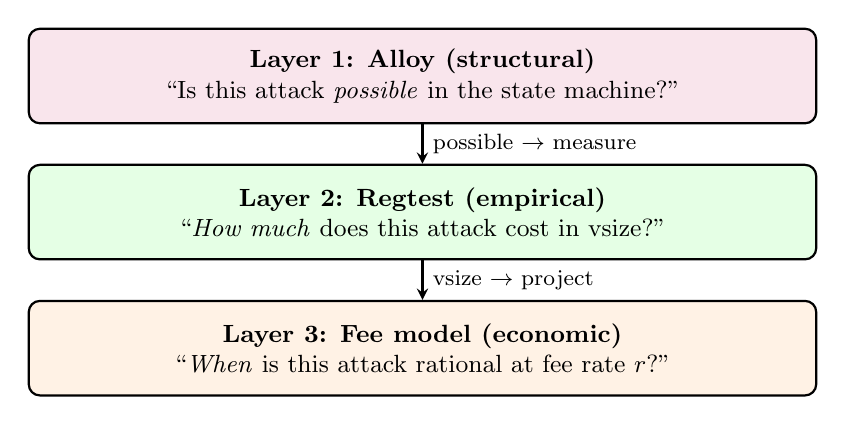
\begin{tikzpicture}[
  layer/.style={rectangle, draw, rounded corners=4pt, minimum width=10cm,
                minimum height=1.2cm, font=\small, align=center},
  >=stealth, thick,
]
  \node[layer, fill=purple!10] (alloy)
    {\textbf{Layer 1: Alloy (structural)}\\
     ``Is this attack \emph{possible} in the state machine?''};
  \node[layer, fill=green!10, below=0.5cm of alloy] (regtest)
    {\textbf{Layer 2: Regtest (empirical)}\\
     ``\emph{How much} does this attack cost in vsize?''};
  \node[layer, fill=orange!10, below=0.5cm of regtest] (fee)
    {\textbf{Layer 3: Fee model (economic)}\\
     ``\emph{When} is this attack rational at fee rate~$r$?''};

  \draw[->] (alloy) -- node[right, font=\footnotesize] {possible $\rightarrow$ measure} (regtest);
  \draw[->] (regtest) -- node[right, font=\footnotesize] {vsize $\rightarrow$ project} (fee);
\end{tikzpicture}
\caption{Three-layer evidence methodology. Alloy determines structural possibility.
Regtest measures concrete costs. The fee model projects costs into real-world
fee environments to determine economic rationality.}
\label{fig:three_layer}
\end{figure}

\begin{itemize}
\item \textbf{Layer 1 (Alloy): Is the attack structurally possible?}
  If the Alloy check passes (no counterexample), the attack is structurally
  impossible within the modeled scope. If a counterexample is found, the attack
  is possible and proceeds to Layer~2.

\item \textbf{Layer 2 (Regtest): How much does it cost?}
  The regtest experiments measure the concrete vsize of the attack and defense
  transactions, converting a structural possibility into a quantitative cost.

\item \textbf{Layer 3 (Fee model): When is it rational?}
  The fee projection model (Equation~\ref{eq:fee_projection}) converts vsize into
  sats at each fee rate, and the rationality condition
  (Equation~\ref{eq:rationality}) determines when the attack is economically justified.
\end{itemize}

Table~\ref{tab:three_layer} illustrates the alignment for three representative attacks.

\begin{table}[t]
\centering
\caption{Three-layer evidence alignment for representative attacks.}
\label{tab:three_layer}
\small
\begin{tabular}{@{}lp{2.5cm}p{3cm}p{3.5cm}@{}}
\toprule
Attack & Alloy (Layer 1) & Regtest (Layer 2) & Fee model (Layer 3) \\
\midrule
CCV griefing (TM2)
  & Reachable (keyless recovery exists)
  & 122\vB{}/round attacker, 454\vB{}/round defender
  & Rational at all fee rates; $\gamma = 0.27$ \\[6pt]

CTV fee pinning (TM1)
  & Reachable (anchor output spendable)
  & 14{,}300~sats total
  & Rational whenever vault $> 20{,}000$~sats \\[6pt]

CAT+CSFS cold theft (TM11)
  & Counterexample found (cold key extracts)
  & 125\vB{} recovery tx
  & Rational at any fee rate (immediate theft) \\
\bottomrule
\end{tabular}
\end{table}

The three layers reinforce each other: Alloy gives confidence that the regtest
experiments measure the right attacks (no missed paths), the regtest measurements
give concrete costs to the Alloy-identified possibilities, and the fee model
transforms those costs into deployment guidance.

\chapter{Discussion} \label{ch:discussion}

This chapter addresses limitations of the methodology, discusses mitigations for
the vulnerabilities identified, and identifies open problems for future work.

% ======================================================================
\section{Limitations} \label{se:limitations}

\subsection{Regtest Environment}

The regtest limitations detailed in Section~\ref{se:regtest_validity} bound the
external validity of all measurements. The most significant gap is the absence of
temporal dynamics: recovery races between the attacker's withdrawal and the
watchtower's response are instantaneous on regtest but uncertain on mainnet, where
block confirmation times are stochastic and mempool congestion affects transaction
propagation. The No Pareto-Optimal Design theorem
(Proposition~\ref{thm:fee_inversion}) is robust to this gap because its
per-threat orderings rest on structural vsize measurements rather than
timing---but the \emph{practical feasibility} of per-UTXO recovery-cost scaling
at a given fee rate depends on how quickly the attacker can fill
blocks with split transactions, which regtest cannot test.

\subsection{Reference Implementations} \label{se:impl_choices}

This work studies covenant \emph{designs} (BIPs), not implementations. However, the
measurements come from specific reference implementations, and implementation choices
affect the measured vsize. The most significant example is OP\_VAULT's fee-input
requirement: the 292\vB{} trigger measurement includes a fee-wallet input that is
inherent to BIP-345's value preservation rule, not an implementation artifact. But
CTV's 3{,}300-sat anchor output and CAT+CSFS's unconstrained recovery leaf are
implementation choices, not BIP requirements. Table~\ref{tab:impl_choices} lists
the design choices in the two author-built implementations (CAT+CSFS and Simplicity)
that could affect measured properties.

\begin{table}[t]
\centering
\caption{Implementation choices in author-built vaults. These are design decisions,
not BIP requirements; alternative designs would produce different measurements.}
\label{tab:impl_choices}
\small
\begin{tabular}{@{}llll@{}}
\toprule
Choice & Covenant & BIP-required? & Alternative \\
\midrule
Fixed destination        & CAT+CSFS & No  & Poelstra's dynamic destination~\cite{Poe21} \\
Unconstrained recovery   & CAT+CSFS & No  & Output-constrained (like Simplicity) \\
MAX\_FEE cap (in-value) & Simplicity & No & Fully dynamic signer-side fee selection without cap \\
3{,}300-sat anchor       & CTV (upstream) & No & Different anchor size \\
\bottomrule
\end{tabular}
\end{table}

\subsection{Rational Adversary Assumption}

The economic analysis assumes a rational adversary who mounts an attack only when
$\text{attack\_cost} < \text{vault\_value}$. This excludes irrational adversaries
(state actors, ideologically motivated attackers) who may attack regardless of cost.
It also excludes sophisticated attackers who combine covenant-level attacks with
network-level attacks (eclipse, time-dilation) to improve their success probability.

\subsection{Threats Not Modeled} \label{se:threats_not_modeled}

The TM1--TM11 threat taxonomy covers covenant-specific attack classes but excludes
several categories that apply equally to all vault designs:

\begin{itemize}
\item \textbf{TM3 race dynamics are network-layer, not Script-layer.}
  Our design-space decomposition
  (Section~\ref{ss:design_space}) does not model the race between
  the attacker's unvault-plus-withdrawal sequence and the
  watchtower's recovery broadcast. Formalising
  $\Pr_D[\text{attacker wins race}]$ would require a separate
  probability space over block-arrival times, mempool propagation
  delays, and detection latency---parameters that depend on the
  deployment environment (mainnet, regtest, signet) rather than on
  BIP script semantics. Existing watchtower and payment-channel
  formalisations in the state-channel literature treat confirmation
  as atomic or assume bounded-delay synchrony; none provides
  off-the-shelf machinery for a pinning-composed race against
  a Bitcoin mempool. We therefore treat TM3 as uniformly
  applicable to all four BIPs at the Script layer. CAT+CSFS's
  dual-binding on the hot leaf is the one design-level mitigation
  in our taxonomy: it reduces the worst-case outcome from theft to
  griefing (see Section~\ref{se:trigger_theft}). A formal network-layer
  race model is left for future work.

\item \textbf{Mining-level attacks.} An attacker with significant hash power could
  withhold blocks to compress CSV timelocks, reducing the watchtower's response
  window. This interacts with TM3 and TM4 but is not covenant-specific.

\item \textbf{Network-level attacks.} Eclipse attacks could prevent a watchtower from
  observing unvault transactions, giving the attacker a head start on the CSV race.

\item \textbf{Watchtower availability.} All vault designs assume the watchtower is
  online during the CSV window. DDoS attacks targeting the watchtower infrastructure
  are a deployment concern orthogonal to covenant design.

\item \textbf{Multisig key management.} Production vaults would use multisig (e.g.,
  2-of-3 cold keys). The interaction between threshold signing schemes and covenant
  enforcement is not addressed.

\item \textbf{Dust limit changes.} The per-UTXO recovery-cost scaling analysis assumes current
  dust limits (${\sim}546$~sats). Changes to dust relay policy would shift the
  economic floor at which splits become unrecoverable.
\end{itemize}

These threats are orthogonal to the covenant-specific properties measured in this
work. They represent important deployment considerations but do not affect the
relative ranking of covenant designs.

% ======================================================================
\section{Mitigations} \label{se:mitigations}

\subsection{TRUC/v3 Transactions}

TRUC (Topologically Restricted Until Confirmation), also known as v3 transactions,
limits descendant chains to a single transaction. TRUC was merged into Bitcoin Core
28.0~\cite{CoreRelay} and is available on mainnet as an opt-in relay policy.
If CTV vault transactions adopt TRUC, the 25-descendant fee pinning vector (TM1)
is eliminated at the relay policy level. This would remove CTV's primary
vulnerability, potentially shifting its
security profile: without fee pinning, CTV's worst-case attack becomes address reuse
(TM7), which is a user error preventable by wallet software rather than an adversarial
exploit. The TM1 row of the master threat matrix (and hence the CTV
branch of Proposition~\ref{thm:fee_inversion}'s counterexample
enumeration) would need re-evaluation under TRUC, as CTV would no
longer have a fee-invariant worst case under~TM1.

\subsection{Batched Recovery}

Class \classscale{} (TM4) is materially mitigated by batching
recovery transactions. Instead of recovering each split UTXO
individually, the watchtower combines multiple UTXOs into a single
recovery transaction, amortising fixed overhead across inputs. We
measure batched recovery on regtest for both CCV and OP\_VAULT
(Section~\ref{ss:batched_defender}); the fitted linear scaling is
$54 + 68 N$\vB{} for CCV and $154 + 92 N$\vB{} for OP\_VAULT. The
dust-threshold fee rate~$r^\dagger$ rises by $1.8\times$~(CCV) and
$2.7\times$~(OP\_VAULT), and the CCV/OP\_VAULT ordering under TM4
reverses relative to the single-input case.

\subsection{Poelstra Reset Model}

CAT+CSFS's cold key vulnerability (TM11) can be mitigated by replacing the bare
\texttt{OP\_CHECKSIG} recovery leaf with a recursive staging reset, as proposed by
Poelstra~\cite{Poe21}. Under this design, cold key compromise initiates a liveness
battle: the attacker resets the vault, the owner triggers a new withdrawal, the
attacker resets again. Each round costs both parties transaction fees. This converts
immediate theft into sustained denial of service, matching OP\_VAULT's security
profile under dual-key compromise. The tradeoff is a larger recovery script and
additional witness overhead.

% ======================================================================
\section{Open Problems} \label{se:open_problems}

\paragraph{Temporal verification.}
The Alloy models verify structural reachability but not timing properties. A TLA+
or UPPAAL model could capture the recovery race dynamics: given a CSV delay of
$d$~blocks, a block interval distribution, and network propagation delays, what is
the probability that the watchtower's recovery confirms before the attacker's
withdrawal? This would complement the structural verification with probabilistic
timing guarantees.

\paragraph{Cryptographic verification.}
The Alloy models abstract signatures as key-possession checks. A Tamarin or ProVerif
model could verify the cryptographic binding properties: that the CAT+CSFS dual
verification is sound under the Schnorr signature scheme, that CTV template hashes
are collision-resistant under SHA-256, and that Simplicity's jet-based verification
is equivalent to the combinator semantics. O'Connor's Coq formalization of
Simplicity~\cite{OC17} provides a foundation for this direction.

\paragraph{Cluster mempool impact.}
The ongoing Bitcoin Core cluster mempool redesign replaces per-transaction
ancestor/descendant limits with cluster-based evaluation~\cite{WD24}. This could
fundamentally change the fee pinning calculus: the 25-descendant limit exploited in
TM1 may be replaced by cluster size limits with different eviction logic. Measuring
the fee pinning attack under cluster mempool rules would determine whether CTV's
primary vulnerability survives the policy change.

\paragraph{Replacement cycling.}
Riard~\cite{Ria23} demonstrated transaction replacement cycling attacks against
Lightning Network HTLCs. The same class of attack may apply to covenant vaults:
an attacker could cycle the watchtower's recovery transaction out of the mempool
by repeatedly replacing it with conflicting transactions. This interaction between
covenant security and mempool replacement policy is unexplored.

\paragraph{Multi-vault composition.}
Real-world deployments would use multiple vaults simultaneously. The interaction
between concurrent vault operations---fee wallet contention in OP\_VAULT, UTXO set
management across vaults, and cross-vault batching opportunities---introduces
composition effects not captured by single-vault analysis.

\chapter{Related Work} \label{ch:related}

This chapter positions our work relative to prior research on Bitcoin vault custody,
covenant design, formal verification of cryptocurrency protocols, and layer-two
security.

% ======================================================================
\section{Vault Custody Protocols} \label{se:rw_vault_custody}

Swambo et al.~\cite{SHMB20} formalized the vault lifecycle model---deposit, unvault,
withdraw, recover---and the watchtower monitoring assumption that underpins all
covenant vault designs. Their analysis established the threat vocabulary (key
compromise, liveness denial, fund safety) that we adopt and extend with the
11-threat taxonomy (TM1--TM11). A companion paper~\cite{SBMB20} characterized three
approaches to implementing covenants (pre-signed transactions with deleted keys,
OP\_CHECKOUTPUTSHASHVERIFY, and OP\_CHECKTEMPLATEVERIFY), analyzing the security
assumptions of each. Their work analyzed deleted-key covenants and pre-signed
transaction vaults without comparing opcode-level designs empirically. Swambo's
doctoral thesis~\cite{Swa23} extended this to the Ajolote autonomous custody system
with formal security analysis, but did not include CTV, CCV, OP\_VAULT, or
CAT+CSFS.

M\"oser, Eyal, and G\"un Sirer~\cite{MES16} introduced covenants as a mechanism for
vault-based custody, proposing script-level restrictions on how UTXOs can be spent.
Their work predates all four BIP proposals studied here and provides the conceptual
foundation for the covenant approach to custody. O'Connor and
Piekarska~\cite{OP17} demonstrated that covenants can be implemented in Bitcoin by
adding OP\_CAT and OP\_CHECKSIGFROMSTACKVERIFY, foreshadowing the CAT+CSFS design
studied in this thesis.

O'Beirne's technical report on vaults and covenants~\cite{OBeirne23} provides a
practitioner-oriented comparison of vault designs, analyzing the tradeoffs between
OP\_VAULT's purpose-built approach and CTV's generic template commitment. This
informed the design of BIP-345~\cite{BIP345}, which was subsequently
withdrawn~\cite{OB25} in favor of CCV (BIP-443).

Kirstein et al.~\cite{KLGZ21} proposed Phoenix, a formally verified regenerating
vault that recovers from key compromise by regenerating the vault with new keys.
Their work uses formal verification (in Dafny) to prove safety properties of a
single vault design. Our work differs by comparing five designs under a uniform
methodology rather than deeply verifying one.

The Bitcoin PIPEs v2 proposal~\cite{PIPES26} introduces an alternative approach to
covenants using zero-knowledge proofs, enabling programmable vaults without new
opcodes. This represents a fundamentally different design philosophy from the
opcode-level covenants studied here.

% ======================================================================
\section{Covenant Proposals and Analysis} \label{se:rw_covenants}

Each covenant proposal has its own design documentation and community analysis, but
no prior work compares them empirically.

Rubin~\cite{BIP119} specified CTV and discussed its applications (vaults, congestion
control, payment pools) but did not provide measured transaction sizes or cross-design
comparisons. The bitcoin-dev mailing list discussion identified address reuse as a
risk, which we confirm empirically.

Ingala~\cite{BIP443} designed CCV (originally MATT) and documented the keyless recovery
griefing concern and the OP\_SUCCESS behavior for undefined modes. Our work quantifies
the griefing cost asymmetry ($\gamma = 0.27$) and confirms the OP\_SUCCESS behavior
across five undefined mode values on a production-shaped taptree.

O'Beirne and Sanders~\cite{BIP345} specified OP\_VAULT with authorized recovery and
automatic revault. Harding~\cite{Har24} estimated per-UTXO recovery-cost scaling at
approximately 3{,}000 splits per block. We confirm this for OP\_VAULT (3{,}427
measured) and extend it to CCV (6{,}172 splits per block, 80\% more than Harding's
estimate). O'Beirne subsequently withdrew BIP-345~\cite{OB25}; our lifecycle cost
comparison (OP\_VAULT 36\% more expensive than CCV) provides quantitative context for
that decision.

Poelstra~\cite{Poe21} demonstrated transaction introspection via OP\_CAT and Schnorr
signature tricks, constructing a vault with recursive covenants and dynamic destination
selection. Our CAT+CSFS vault implements a simplified variant (fixed destination, no
recursion) to isolate the dual-verification security properties. The cold key recovery
vulnerability (TM11) and the Poelstra reset cost model in Chapter~\ref{ch:security}
directly build on this work. Rijndael~\cite{Rij24} built a working vault prototype
using only OP\_CAT and the Schnorr G-trick (without CSFS), demonstrating that OP\_CAT
alone enables covenant enforcement.

% ======================================================================
\section{Formal Verification of Bitcoin Contracts} \label{se:rw_formal}

Bartoletti and Zunino~\cite{BZ18} introduced BitML, a domain-specific calculus for
Bitcoin smart contracts with formal semantics based on process algebra. BitML enables
reasoning about contract security through symbolic and computational models.
Subsequent work developed a toolchain for compiling BitML to Bitcoin
transactions~\cite{ABL19} and verified liquidity properties of recursive
contracts~\cite{BLM22}. Bartoletti, Lande, and Zunino~\cite{BLZ20} extended this
line to Bitcoin covenants, modeling vault contracts in an extended BitML with
covenant primitives and proving safety properties. Our Alloy models operate at a
different abstraction level---state-machine reachability rather than process-algebraic
semantics---but address the same class of questions: can an attacker extract funds
from a correctly constructed vault?

dgpv~\cite{dgpv24} applied Alloy bounded model checking to Rijndael's OP\_CAT vault
prototype, verifying fund conservation and covenant enforcement properties within
a single design. Our work extends this methodology to all four BIP-specified
designs plus Simplicity, using a shared base model (\texttt{vault\_base.als}) to
ensure uniform property definitions. We add the threat model layer
(\texttt{threat\_model.als}) for systematic attacker profiling and the cross-covenant
module (\texttt{cross\_covenant.als}) for multi-design interaction
checking---neither of which appears in dgpv's analysis.

O'Connor~\cite{OC17} provided Coq-verified denotational semantics for the Simplicity
language, establishing the formal foundation for reasoning about Simplicity programs.
Our Alloy model of the Simplicity vault operates at the state-machine level (vault
lifecycle transitions) rather than the language semantics level, complementing
O'Connor's foundational work with application-level verification. O'Connor and
Poelstra have also pursued formal verification of cryptographic primitives used in
Bitcoin's libsecp256k1 library using Coq, demonstrating the viability of machine-checked
proofs for Bitcoin infrastructure.

Several surveys have cataloged formal verification methods for blockchain smart
contracts. Murray and Anisi~\cite{Murray19} categorized approaches including model
checking, theorem proving, and symbolic execution. Tolmach et al.~\cite{Tolmach21}
provided a comprehensive survey of formal specification and verification techniques,
covering 50+ tools and frameworks. Almakhour et al.~\cite{Almakhour20} focused on
verification methods applicable to production smart contracts, and Singh
et al.~\cite{Singh20} analyzed how formalization approaches address known
vulnerability classes. Our use of Alloy bounded model checking falls within the model
checking category identified by these surveys, applied specifically to Bitcoin
covenant protocols rather than Ethereum smart contracts.

% ======================================================================
\section{Layer-Two Security and Watchtower Economics} \label{se:rw_layer2}

The watchtower monitoring model used in vault security is closely related to the
watchtower concept in Lightning Network payment channels. Leinweber
et al.~\cite{LGSM19} proposed TEE-based distributed watchtowers for fraud protection
in Lightning, analyzing the economic viability of third-party watchtower services.
Our per-UTXO recovery-cost scaling analysis (TM4) addresses a different question---how an
attacker can exhaust the watchtower's recovery budget through vault
splitting---but shares the assumption of an always-online monitoring service.

Naumenko and Riard~\cite{NR21} analyzed time-dilation attacks on the Lightning
Network, where an attacker with network-level capabilities manipulates the victim's
view of the blockchain to compress timelocks. This attack class applies to covenant
vaults (an attacker could compress the CSV window), but we do not model it because
it is orthogonal to covenant-specific properties and requires network-layer
simulation beyond our regtest methodology. Riard~\cite{Ria23} subsequently
demonstrated replacement cycling attacks against Lightning HTLCs, a mempool
manipulation technique that may also apply to covenant vault recovery transactions.

Aumayr~\cite{Aumayr24} provided a comprehensive formal treatment of
Bitcoin-compatible scalability protocols, including watchtower collateralization
and channel closing security. The economic analysis of watchtower reserves in that
work parallels our per-UTXO recovery-cost scaling budget calculations, though applied to
payment channels rather than vaults.

% ======================================================================
\section{Qualitative Comparisons} \label{se:rw_qualitative}

The covenants.info website~\cite{covenants_info} provides a qualitative feature matrix
comparing covenant proposals across dimensions such as recursion support, introspection
granularity, and application breadth. This resource contains no transaction sizes, no
attack cost functions, and no fee-environment analysis. Our work complements it with
quantitative measurements.

The B-SSL covenant-free vault model~\cite{BSSL25} demonstrates vault-like custody
using only CSV and CLTV timelocks (no new opcodes). This provides a baseline for
what is achievable without covenants---the security properties are weaker (no output
constraints on recovery, no dynamic destination selection) but the deployment path
requires no consensus changes.

% ======================================================================
\section{Summary of Positioning} \label{se:rw_positioning}

Table~\ref{tab:related_work} compares this work with the most closely related prior
efforts across five dimensions.

\begin{table}[t]
\centering
\caption{Comparison with closely related prior work.}
\label{tab:related_work}
\small
\begin{tabular}{@{}lccccc@{}}
\toprule
Work & Covenants & Empirical? & Formal? & Fee analysis? & Year \\
\midrule
M\"oser et al.~\cite{MES16}      & 1 (generic)
  & No  & No & No  & 2016 \\
Swambo et al.~\cite{SHMB20}  & 0\textsuperscript{a}
  & No  & Partial & No  & 2020 \\
Bartoletti et al.~\cite{BLZ20}   & 1 (BitML)
  & No  & Yes (process) & No  & 2020 \\
Kirstein et al.~\cite{KLGZ21}    & 1 (Phoenix)
  & No  & Yes (Dafny) & No  & 2021 \\
Harding~\cite{Har24}          & 1 (OPV)
  & No\textsuperscript{b}  & No & Partial & 2024 \\
dgpv~\cite{dgpv24}            & 1 (CAT)
  & No  & Yes (Alloy) & No  & 2024 \\
covenants.info~\cite{covenants_info} & 6+
  & No  & No & No  & 2024 \\
\textbf{This work}            & \textbf{5}
  & \textbf{Yes} & \textbf{Yes (Alloy)} & \textbf{Yes} & \textbf{2026} \\
\bottomrule
\multicolumn{6}{@{}l}{\footnotesize \textsuperscript{a}Analyzes vault model
generically, not specific BIP opcodes.} \\
\multicolumn{6}{@{}l}{\footnotesize \textsuperscript{b}Estimates from assumed
transaction sizes, not regtest measurements.}
\end{tabular}
\end{table}

No prior work combines empirical measurement, formal verification, and
fee-environment-dependent security analysis for multiple covenant vault designs.
The individual components---vault lifecycle modeling~\cite{SHMB20}, Bitcoin contract
formalization~\cite{BZ18, BLZ20}, Alloy verification~\cite{dgpv24}, watchtower
exhaustion estimation~\cite{Har24}---exist in isolation. Our contribution is the
integration of these approaches under a uniform methodology that enables cross-design
comparison and the derivation of results (Proposition~\ref{thm:griefing_safety}
and~\ref{thm:fee_inversion}) that require data from multiple designs simultaneously.

\chapter{Conclusion} \label{ch:conclusion}

This thesis presented the first empirical comparison of four Bitcoin covenant vault
designs---CTV (BIP-119), CCV (BIP-443), OP\_VAULT (BIP-345), and CAT+CSFS
(BIP-347 + BIP-348)---plus a fifth vault built with the Simplicity language on
Elements. Through 15 experiments on regtest, Alloy formal verification, and
parameterized economic modeling, we established two results that constrain the
design space of covenant vaults.

\paragraph{Result 1: Griefing--safety impossibility.}
No covenant vault simultaneously achieves permissionless recovery and griefing
resistance (Proposition~\ref{thm:griefing_safety}). This is a structural design
constraint, not an implementation limitation. Vault designers must choose between
maximizing fund safety under key loss (CCV's keyless recovery) and minimizing
denial-of-service exposure (OP\_VAULT's authorized recovery).

\paragraph{Result 2: Structural design-space decomposition.}
Covenant vault designs are characterised by four nearly-orthogonal
dimensions: fee model ($f$), amount flexibility ($a$), recovery
gating ($g$), and recovery binding ($b$). Each dimension carries a
deterministic feature-to-vulnerability implication
(Lemmas~\ref{lem:anchor_pinning}--\ref{lem:unbound_theft}): the
anchor-output fee model opens TM1 (fee pinning); partial-withdrawal
flexibility opens TM4 (per-UTXO recovery-cost scaling); keyless recovery
opens TM2 (permissionless griefing, by
Proposition~\ref{thm:griefing_safety}); and unbound recovery opens
TM11 (cold-key theft for the full vault value).
Proposition~\ref{thm:fee_inversion} establishes that no proposed
Bitcoin Script extension occupies the dominant design-space corner
$(f_{\neq\text{anchor}}, a_{\text{atomic}}, g_{\text{key}},
b_{\text{bound}})$ at which $\mathcal{L} = 0$ simultaneously across
\{TM1, TM2, TM4, TM11\}. Every proposal differs from the corner in
at least one dimension, and by the corresponding lemma that
difference forces a positive defender loss on the threat that the
dimension controls. The decomposition also provides a framework for
localising future BIPs in the lattice: their vulnerability profile
follows from their feature tuple without further measurement.

\paragraph{Empirical corrections.}
We corrected prior hand-estimates of OP\_VAULT transaction sizes by 45--46\%
(trigger: $200 \rightarrow 292$\vB{}, recovery: $170 \rightarrow 246$\vB{}),
revealing a 36\% lifecycle cost premium over CCV. We measured CCV's watchtower
splitting capacity at approximately 6{,}172 splits per block---80\% more than
Harding's estimate of ${\sim}3{,}000$, which assumed OP\_VAULT-sized transactions.
These are the first regtest-validated vsize measurements for all four Bitcoin
covenant vault lifecycles.

\paragraph{Batched recovery and ordering flip.}
BIP-345's ``Batching'' section (authorised recovery, lines~613--621)
and BIP-443's default aggregation mode permit the defender to recover
$N$ Unvaulting UTXOs in a single transaction. Measured on regtest, the
amortised per-input cost is $68$\vB{} for CCV and $92$\vB{} for
OP\_VAULT. The dust-threshold fee rate rises by $1.8\times$ and
$2.7\times$ respectively, and the relative vulnerability of the two
designs under TM4 reverses: CCV is safer single-input, OP\_VAULT is
safer batched (Section~\ref{ss:batched_defender}).

\paragraph{Original implementations.}
We built a CAT+CSFS vault using explicit \texttt{OP\_CHECKSIGFROMSTACK}
(BIP-348) dual verification---distinct from prior OP\_CAT-only vaults
that use the Schnorr G-trick without CSFS~\cite{Poe21, Rij24}---and a
Simplicity vault on Elements using jet-based covenant enforcement.
Both are open-source. The CAT+CSFS implementation revealed the cold
key recovery vulnerability (TM11): bare \texttt{OP\_CHECKSIG} recovery
grants immediate, unrestricted fund theft upon cold key compromise.
The Simplicity vault serves as a cross-substrate reference point,
showing output-constrained recovery on all paths under the federated
sidechain trust model.

\paragraph{Formal verification.}
Alloy bounded model checking verified fund conservation, recovery
liveness, and no-extraction properties across the four Bitcoin Script
extension designs plus the Simplicity reference. The one expected
assertion failure---cold key extraction in CAT+CSFS---structurally
confirms TM11. The three-layer evidence methodology (Alloy for
structural possibility, regtest for concrete cost, fee model for
economic rationality) provides complementary assurance that no single
analysis technique could achieve alone.

\section{Future Work}

Several directions extend this research:

\begin{itemize}
\item \textbf{TRUC/v3 impact.} If adopted, TRUC transactions would eliminate CTV's
  descendant-chain fee pinning, removing its primary vulnerability and requiring
  re-evaluation of the TM1 branch of
  Proposition~\ref{thm:fee_inversion}'s counterexample enumeration.

\item \textbf{Cluster mempool.} The Bitcoin Core cluster mempool redesign may change
  descendant limit semantics, affecting the fee pinning attack construction.

\item \textbf{Temporal verification.} TLA+ or UPPAAL models could verify recovery
  race timing properties that Alloy's state-machine abstraction cannot capture.

\item \textbf{CTV+CSFS activation.} As CTV and CSFS move toward activation signaling,
  the measurements and cost models in this work can inform deployment decisions.
  The fee-conditional guidance (Section~\ref{se:deployment}) is directly applicable
  to vault designers choosing between CTV-only and CAT+CSFS vaults.

\item \textbf{Multi-vault composition.} Production deployments managing multiple
  concurrent vaults introduce fee wallet contention, cross-vault batching
  opportunities, and UTXO management complexity not captured by single-vault analysis.
\end{itemize}

The framework, all measurements, formal models, and both original vault
implementations are available at
\url{https://github.com/PraneethGunas/covenant-vault-research}.


% ── Bibliography ──────────────────────────────────────────────
% EXCLUDED for iThenticate per VT Graduate School instructions
%\bibliography{references}
%\bibliographystyle{plainnat}

% ── Appendix ──────────────────────────────────────────────────
\appendix
\begin{appendices}
  \chapter{Alloy Model Details} \label{app:alloy_details}

This appendix provides the model architecture, per-module descriptions, and
detailed per-covenant verification results summarized in
Chapter~\ref{ch:verification}.

% ======================================================================
\section{Model Architecture}

The Alloy models follow a three-layer inheritance hierarchy
(Figure~\ref{fig:alloy_hierarchy}).

\begin{figure}[t]
\centering
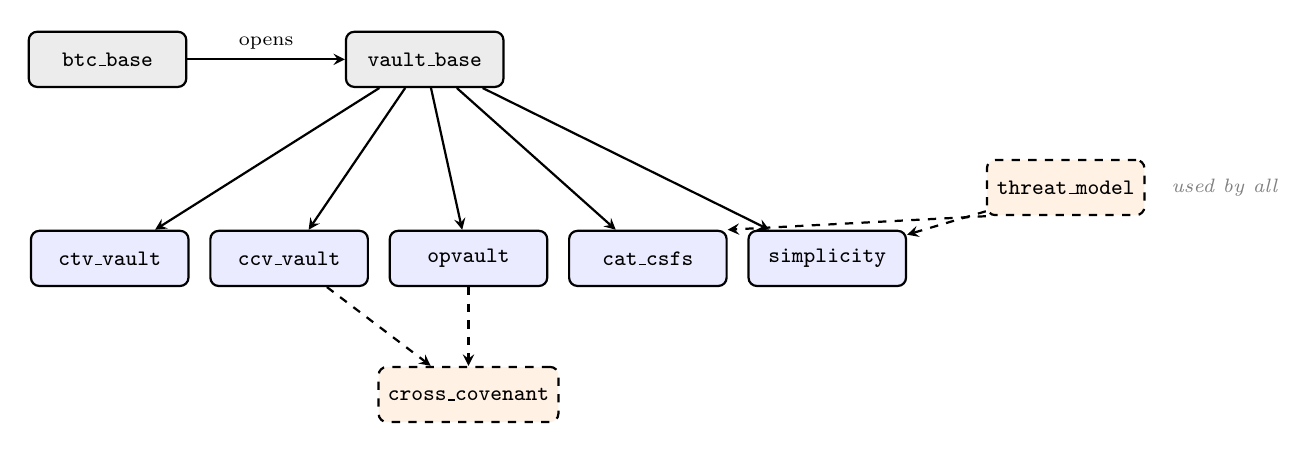
\begin{tikzpicture}[
  box/.style={rectangle, draw, rounded corners=3pt, minimum width=2cm,
              minimum height=0.7cm, font=\footnotesize, align=center},
  base/.style={box, fill=gray!15},
  concrete/.style={box, fill=blue!8},
  cross/.style={box, fill=orange!10, dashed},
  >=stealth, thick,
  node distance=0.6cm,
]
  \node[base] (btc) {\texttt{btc\_base}};
  \node[base, right=2cm of btc] (vault) {\texttt{vault\_base}};
  \draw[->] (btc) -- node[above, font=\scriptsize] {opens} (vault);

  \node[concrete, below=1.8cm of vault, xshift=-4cm] (ctv)
    {\texttt{ctv\_vault}};
  \node[concrete, right=0.25cm of ctv] (ccv)
    {\texttt{ccv\_vault}};
  \node[concrete, right=0.25cm of ccv] (opv)
    {\texttt{opvault}};
  \node[concrete, right=0.25cm of opv] (cat)
    {\texttt{cat\_csfs}};
  \node[concrete, right=0.25cm of cat] (sim)
    {\texttt{simplicity}};

  \foreach \c in {ctv, ccv, opv, cat, sim}
    \draw[->] (vault) -- (\c);

  \node[cross, right=1cm of sim, yshift=0.9cm] (threat)
    {\texttt{threat\_model}};
  \draw[->, dashed] (threat) -- (sim);
  \draw[->, dashed] (threat.south west) -- (cat.north east);

  \node[cross, below=1cm of opv] (cross)
    {\texttt{cross\_covenant}};
  \draw[->, dashed] (ccv) -- (cross);
  \draw[->, dashed] (opv) -- (cross);

  \node[font=\scriptsize, text=gray, anchor=west] at (threat.east)
    [xshift=0.2cm] {\itshape used by all};
\end{tikzpicture}
\caption{Alloy model hierarchy. \texttt{btc\_base} defines UTXOs, keys, and
transactions. \texttt{vault\_base} defines the abstract vault state machine.
Five concrete models extend the base with covenant-specific transition guards.
\texttt{threat\_model} and \texttt{cross\_covenant} are cross-cutting modules.}
\label{fig:alloy_hierarchy}
\end{figure}

\paragraph{\texttt{btc\_base.als}.}
Defines the Bitcoin transaction model: signatures for \texttt{UTXO}, \texttt{Key},
\texttt{Transaction}, and \texttt{Address}. UTXOs have an amount, owner key, and
spent status. Transactions consume inputs and produce outputs. This module provides
the vocabulary shared by all vault models.

\paragraph{\texttt{vault\_base.als}.}
Defines the abstract vault state machine: four states (\texttt{VAULTED},
\texttt{UNVAULTING}, \texttt{WITHDRAWN}, \texttt{RECOVERED}), transitions between
states (trigger, withdraw, recover), and the \texttt{VaultFamily} concept that groups
UTXOs belonging to the same vault instance. The CSV delay is modeled as an integer
field on each vault UTXO. Properties defined at this level (fund conservation,
recovery liveness) apply uniformly to all concrete models.

\paragraph{Concrete vault models.}
Each of the five models extends \texttt{vault\_base} with covenant-specific
transition guards. \texttt{ccv\_vault} models the CCV mode enumeration
and the OP\_SUCCESS behavior for undefined modes. \texttt{opvault\_vault} models
the three-key separation and authorized recovery. \texttt{cat\_csfs\_vault} models
the dual-verification binding and unconstrained recovery leaf.

\paragraph{\texttt{threat\_model.als}.}
Defines attacker profiles by specifying which keys the attacker controls. Properties
are checked under each profile to determine the minimum capability needed for each
attack class.

\paragraph{\texttt{cross\_covenant.als}.}
Models interactions between vault instances from different covenant types sharing the
same UTXO set. Checks whether cross-vault injection is possible and whether fee
wallet contention between concurrent OP\_VAULT operations can block recovery.

% ======================================================================
\section{Per-Covenant Detailed Results}

\paragraph{CTV.}
All six checks pass: no unauthorized extraction (with no keys and with hot key only),
CSV enforcement, no state proliferation, eventual withdrawal, and recovery liveness.
The address reuse scenario finds an instance where a second deposit creates an
unspendable UTXO, confirming the structural vulnerability (TM7).

\paragraph{CCV.}
All seven checks pass, including the mode confusion containment check (undefined
modes trigger OP\_SUCCESS but only within the affected leaf---the vault's other
leaves remain secure). The griefing scenario demonstrates that any party can invoke
recovery without keys (TM2). The splitting scenario shows the revault chain that
enables the per-UTXO recovery-cost scaling of class Z3 (TM4).

\paragraph{OP\_VAULT.}
All eight checks pass, including the dual-key-no-theft property (trigger +
recoveryauth compromise produces liveness denial but not fund theft, because the
recovery address is pre-committed). The key-loss scenario demonstrates permanent
inability to recover if the recoveryauth key is destroyed.

\paragraph{CAT+CSFS.}
Five of six checks pass. The \texttt{catcsfsNoExtraction\_ColdKeyOnly} check
\emph{fails}: the Alloy Analyzer finds a trace where the cold key holder invokes
recovery with an attacker-controlled output address, extracting funds. This is the
structural confirmation of TM11 and the only expected assertion failure across all
models. The destination lock and CSV enforcement checks pass.

\paragraph{Simplicity.}
All six checks pass: no extraction under any single-key compromise, output binding
enforcement, CSV enforcement, and no state proliferation. The recovery-constrained
scenario confirms that cold key compromise can only recover to the pre-committed
address (unlike CAT+CSFS).

% ======================================================================
\section{Limitations of the Formal Models}

The Alloy models operate at the state-machine level, abstracting away cryptographic
primitives, serialization details, and temporal dynamics. Signatures are modeled as
key-possession checks (if the attacker holds the key, the signature succeeds). Hash
functions are assumed collision-resistant. Network propagation, mining centralization,
and mempool dynamics are not modeled. These abstractions mean the Alloy verification
confirms \emph{structural} properties (state reachability, authorization requirements)
but not \emph{cryptographic} properties (signature unforgeability, hash binding) or
\emph{temporal} properties (race conditions, confirmation timing). The regtest
experiments partially compensate for the temporal gap by demonstrating actual
transaction construction and broadcast, while the cryptographic properties are
inherited from the underlying BIP-340 Schnorr and SHA-256 specifications.

\end{appendices}

\end{document}
